%% Copernicus Publications Manuscript Preparation Template for LaTeX Submissions
%% ---------------------------------
%% This template should be used for copernicus.cls
%% The class file and some style files are bundled in the Copernicus Latex Package, which can be downloaded from the different journal webpages.
%% For further assistance please contact Copernicus Publications at: production@copernicus.org
%% https://publications.copernicus.org/for_authors/manuscript_preparation.html


%% Please use the following documentclass and journal abbreviations for preprints and final revised papers.

%% 2-column papers and preprints
\documentclass[bg, manuscript]{copernicus}



%% Journal abbreviations (please use the same for preprints and final revised papers)


% Advances in Geosciences (adgeo)
% Advances in Radio Science (ars)
% Advances in Science and Research (asr)
% Advances in Statistical Climatology, Meteorology and Oceanography (ascmo)
% Annales Geophysicae (angeo)
% Archives Animal Breeding (aab)
% ASTRA Proceedings (ap)
% Atmospheric Chemistry and Physics (acp)
% Atmospheric Measurement Techniques (amt)
% Biogeosciences (bg)
% Climate of the Past (cp)
% DEUQUA Special Publications (deuquasp)
% Drinking Water Engineering and Science (dwes)
% Earth Surface Dynamics (esurf)
% Earth System Dynamics (esd)
% Earth System Science Data (essd)
% E&G Quaternary Science Journal (egqsj)
% European Journal of Mineralogy (ejm)
% Fossil Record (fr)
% Geochronology (gchron)
% Geographica Helvetica (gh)
% Geoscience Communication (gc)
% Geoscientific Instrumentation, Methods and Data Systems (gi)
% Geoscientific Model Development (gmd)
% History of Geo- and Space Sciences (hgss)
% Hydrology and Earth System Sciences (hess)
% Journal of Bone and Joint Infection (jbji)
% Journal of Micropalaeontology (jm)
% Journal of Sensors and Sensor Systems (jsss)
% Magnetic Resonance (mr)
% Mechanical Sciences (ms)
% Natural Hazards and Earth System Sciences (nhess)
% Nonlinear Processes in Geophysics (npg)
% Ocean Science (os)
% Primate Biology (pb)
% Proceedings of the International Association of Hydrological Sciences (piahs)
% Scientific Drilling (sd)
% SOIL (soil)
% Solid Earth (se)
% The Cryosphere (tc)
% Weather and Climate Dynamics (wcd)
% Web Ecology (we)
% Wind Energy Science (wes)


%% \usepackage commands included in the copernicus.cls:
%\usepackage[german, english]{babel}
%\usepackage{tabularx}
%\usepackage{cancel}
%\usepackage{multirow}
%\usepackage{supertabular}
%\usepackage{algorithmic}
%\usepackage{algorithm}
%\usepackage{amsthm}
%\usepackage{float}
%\usepackage{subfig}
%\usepackage{rotating}

\graphicspath{{pictures/}}

\begin{document}

%\title{The 2018 heatwave and its implications on ozone induced damage on vegetation in a subarctic climate}
\title{Characterizing subarctic biomes for land surface modeling of pollution and climate risk}


% \Author[affil]{given_name}{surname}

\Author[1]{Stefanie}{Falk}
\Author[2]{Ane Victoria}{Vollsnes}
\Author[2]{Aud E. B.}{Eriksen}
\Author[3]{Lisa}{Emberson}
\Author[3]{Connie}{O'Neill}
\Author[1]{Frode}{Stordal}
\Author[1]{Terje}{Koren Berntsen}

\affil[1]{Department of Geosciences, University of Oslo, Oslo, Norway}
\affil[2]{Department of Biosciences, University of Oslo, Oslo, Norway}
\affil[3]{Department of Environment and Geography, University of York, UK}

%% The [] brackets identify the author with the corresponding affiliation. 1, 2, 3, etc. should be inserted.

%% If an author is deceased, please mark the respective author name(s) with a dagger, e.g. "\Author[2,$\dag$]{Anton}{Aman}", and add a further "\affil[$\dag$]{deceased, 1 July 2019}".

%% If authors contributed equally, please mark the respective author names with an asterisk, e.g. "\Author[2,*]{Anton}{Aman}" and "\Author[3,*]{Bradley}{Bman}" and add a further affiliation: "\affil[*]{These authors contributed equally to this work.}".


\correspondence{Stefanie Falk (stefanie.falk@geo.uio.no)}

\runningtitle{Subarctic biomes for land surface modelling}

\runningauthor{Falk et al.}





\received{}
\pubdiscuss{} %% only important for two-stage journals
\revised{}
\accepted{}
\published{}

%% These dates will be inserted by Copernicus Publications during the typesetting process.


\firstpage{1}

\maketitle


\begin{abstract}
Here we assess the importance of characterization of key meteorological variables and air pollution profiles on the modeled susceptibility of subarctic vegetation to ozone. Changes in climate (e.g. temperature, water availability) will manifest in both direct and indirect effects influencing the species' sensitivity to air pollution. A likely increase in frequency of persistent heatwaves in the future, will inflict heat related stress while generating favorable conditions for the formation of ambient air ozone, e.g. due to wildfires.
We have monitored ambient air ozone concentrations at the Norwegian Institute of Bioeconomy Research (NIBIO) Environment Centre Svanhovd in Northern Norway in the vegetation period 2018/19. Due to data acquisition problems, ozone concentrations for two weeks in July 2018 were missing from our record. We present a reconstruction based on probability density function with respect to the Swedish and Finnish atmospheric monitoring sites and compare with available surface ozone products for the region. Over all, ozone concentrations did not differ significantly between the two years. While temperatures and global irradiance diverged substantially from the multi annual mean precipitation varied only to some extend. 
We investigate the difference in uptake of ozone using the $\mathrm{DO_3SE}$ model, for typical vegetation at the location. We find that bespoke parameterization for subarctic vegetation is essential for an accurate estimation of Phototoxic Ozone Dose (POD) and an assessment of damage risk. Accurate estimates of the start and length of growing season are also crucial.
We find that temperature and its derivative vapor pressure deficit are likely the most important climate variables while the variability of ozone concentration within climatologically reasonable limits plays a minor role.
The use of subarctic parameterization suggests an improvement in risk assessment as POD values are increased in 2018; corroborated by evidence of visible injury in the Svanhovd ozone garden.
\end{abstract}


%\copyrightstatement{TEXT}


\introduction  %% \introduction[modified heading if necessary]
\label{sec:intro}

Ground level ozone is a highly toxic pollutant known to cause damage to a variety of ecosystems around the World \citep{PT:Emberson2020}. At continuously high concentration levels, ozone negatively affects life expectancy of humans \citep{WHO2008} and is a cause of visible injury, photosynthetic damage, early senescence as well as programmed cell death of plants \citep{PCE:Kangasjarvi2005}. Annual global yield losses of four major crops (wheat, rice, maize, and soybean) of $3-15\,\unit{\%}$ \citep{PJ:Ainsworth2017} and a suggested loss in primary production in forestry of $7\,\unit{\%}$ \citep{GCB:Wittig2009,EP:Matyssek2012} has been attributed to ozone. {\bf TODO: Wealth of evidence demonstrating ozone damage to vegetation (perhaps focus on key evidence from northern climates and key species (e.g. birch, Norway srpuce etc... - this might help to make it clear why we focus on these species with the PODy modelling))}
The crop yield loss studies indicate a threat to food security in rapidly developing countries, e.g., in East and South-East Asia \citep{GCB:Tang2013,NCC:Tai2014,AE:Chuwah2015,GCB:Mills2018}, where ozone concentrations related to enhanced pollutant emissions from the transport, residential, power generation and industrial sectors have increased in the past few decades. Even though long-term (pre 1950) observations of surface ozone concentrations are scarce; evidence from trend analysis of those few sites suggests that since the industrial revolution, background concentrations in the northern Hemisphere have at least doubled and continued to increase until relatively recently \citep[Chapter 2]{IPCC2013}. Recent trend analyses indicate that a maximum was reached in 2007 \citep{AE:Derwent2018}, after which tropospheric ozone started to level-off or even decline \citep{ESA:Cooper2014, ACP:Wespes2018,ESA:Gaudel2018}. This can be attributed to a successful implementation of air quality regulations coupled with economic restructuring which saw a move from coal to gas, reduced the number of episodes of peak concentrations especially in summertime over Europe and North America \citep[e.g.,][]{ESA:Fleming2018, ESA:Mills2018}. However, there are indications that an increasing frequency of thermal stress accompanying climate change will reduce vegetations' capacity for ozone uptake and therefor scotch these achievments \citep{NCC:Lin2020}.\\

Ground level ozone is formed in complex photochemical cycles involving precursor gases such as carbon monoxide (\chem{CO}) and hydrocarbons known as volatile organic substances (VOCs) in the presence of nitrogen oxides (\chem{NO_x}). Despite a relatively short tropospheric life-time of approximately $22\,\unit{days}$, ranging from a few days in the tropical boundary layer to up to $1\,\unit{year}$ in the upper troposphere \citep{JGR:Stevenson2005,ACP:Young2013}, ozone is subject to advection over long distances. Episodes of high ozone concentrations in the absence of local pollution sources can therefor often be attributed to long-range transport of both ozone and its precursors. In northern Fennoscandia, episodes of enhanced ozone concentrations in 2003 and 2006 have been traced back to ozone precursor emissions related to forest fires in southern and eastern Europe, respectively \citep{AE:Lindskog2007,EP:Karlsson2013}. In addition, hydrocarbons are also emitted by vegetation itself in form of terpenes and monoterpenes, so called biogenic volatile substances (BVOCs). These emissions are associated with, e.g., thermal stress, defense against herbivores, or even attraction of pollinators \citep{TPS:Penuelas2003}. 

In the annual cycle in boreal and temperate climates, a distinct maximum of ground level ozone concentrations typically occurs in spring followed by lower concentrations throughout the summer. Several conditions unique to the Actic are stimulating the formation of this spring peak. Major pathways of ozone and its precursors' removal from the boundary layer include dry deposition on vegetated surfaces and photochemistry \citep{RG:Clifton2020}. As dry deposition to bare ground or snow and ice covered surfaces was found to be low \citep{ACP:Helmig2007}, both pathways of removal are substantially suppressed during polar night \citep{AE:Monks2000}. This leads to a build up of ozone and its precursors in the course of winter. Come spring precursors are photochemical activated again, while snow cover typically prevails for a longer period of time continuing to suppress ozone dry deposition.
On the other hand, very high ozone concentrations occuring over shorter periodes of time can often be attributed to deep tropopause folding events over the Actic during winter. These events facilitate an intrusion of stratospheric air masses which are enriched in ozone \citep{JGR:Skerlak2015}.
The spring peak is more pronounced in northern Fennoscandia than in more southern locations but shows a  high interannual variability \citep{AB:Klingberg2009, BER:Klingberg2019}. A cause for this is the complex interplay between atmospheric dynamics and chemistry \citep{AE:Laurila1996,BER:Hatakka2003} as described above as well as anthropogenic and biogenic activity \citep{AE:Rummukainen1996,AE:Simpson2002,QJRMS:Galbally2007,NGS:Schnell2009}. \citet{ACP:Andersson2017} showed in a modeling study focused on Fennoscandia that the variability of ozone concentrations in winter can be attributed mainly to changes in atmospheric background (transport) of ozone, while summertime abundance is mostly affected by emissions of precursors in the rest of Europe. Meteorology plays an important role throughout the year.

The start of growing season in northern Fennoscandia has been shifting to earlier dates in response to the general warming trend \citep[e.g.,]{GCB:Menzel2006,RS:Hogda2013,IJB:Karlsen2007} and thereby converging with the period of the ozone spring peak. At the same time the growing season is also becoming longer. In conjunction with midnight sun conditions (almost $24\,\unit{h}$ photosynthetic activity), a longer growing season, is prolonging the time in which vegetation can accumulate ozone. These factors may promote a higher potential susceptibility of northern vegetation to ozone in the future.

Ozone acts as an oxidative stress to plants. Its main action is imposed through reactions occurring in the cell walls and cell membranes of mesophyll cells inside the leaves. Ozone enters the leaves through stomata, that are kept open to allow for gas exchange allowing the entry of \chem{CO_2} for photosynthesis and loss of \chem{H_2O} vapour via the plant transpiration stream. Stomatal aperture, and hence stomatal conductance to these gases (including ozone) will vary over the course of the day and growing season primarily to balance \chem{CO_2} uptake against \chem{H_2O} vapour loss. The higher the stomatal conductance, the higher the potential for ozone uptake. Stomatal conductance has been emperically linked to environmental factors such as air temperature, photosynthetic active radiation, vapor pressure deficit, and soil water potential as well as photosynthesis itself.\\


To measure the risk of damage inflicted to vegetation through ozone, different metrics have been defined. Two main types can be differentiated, concentration-based or flux-based metrics, e.g., Accumulated Over a Threshold $\mathrm{x}$ ($\mathrm{AOT_x}$) and Phyto-toxic Ozone Dose over a threshold $\mathrm{y}$ ($\mathrm{POD_y}$), respectively. Due to their simplicity, concentration-based metrics are still widely used. Despite comparisons of exposure-based methods with previously used concentration based methods (e.g. $\mathrm{AOT_{40}}$) show that $\mathrm{POD_y}$ is better suited to represent the risk to vegetation from ozone, especially in the more climate extreme parts of Europe \citep{GCB:Mills2010,ICP:MappingManual2017}. 

The concentration-based metric $\mathrm{AOT_x}$ (in units of $\unit{ppb}$) is defined as:
\begin{equation}
  \mathrm{AOT_x} = \int{\mathrm{max(\chem{[O_3]}-x)}\cdot \mathrm{dt}},
  \label{eq:aot}
\end{equation}
with the ambient ozone concentration $\chem{[O_3]}$. The  time over which the integration is calculated varies, but is usually defined from $8\,\unit{am}-8\,\unit{pm}$.

For computing the $\mathrm{POD_y}$, an estimate of the stomatal \chem{O_3} flux ($\Phi_\mathrm{sto}$) is calculated based on the assumption that the concentration of \chem{O_3} at the top of the canopy represents a reasonable estimate of the concentration at the upper surface of the laminar layer for a sunlit upper canopy leaf. Details specific to the $\mathrm{DO_3SE}$ model are given in Section~\ref{sec:do3se}. $\mathrm{POD_y}$ is then calculated according to:
%
\begin{equation}
  \mathrm{POD_y} = \int{(\Phi_\mathrm{sto}-y)\cdot \mathrm{dt}},
  \label{eq:pod}
\end{equation}
%
with the hourly averaged ambient air ozone flux through the stomata Eq.~(\ref{eq:flux_stomata}) and a flux threshold $\mathrm{y}$ both given in units of \unit{nmol\,\chem{O_3}\,m^{-2}\,\mathrm{PLA}\,s^{-1}}. The flux threshold $\mathrm{y}$ is representing the detoxification potential of the plant and is typically only exceeded during daylight hours (i.e. when global radiation is above $50\,\unit{W\,m^{-2}}$).

Finally, exceedance of the flux-based critical level (CL) is calculated by:
%
\begin{equation}
  \mathrm{CL_{exeed}} = \mathrm{POD_y} - \mathrm{CL}.
\end{equation}
%

According to a report by the Norwegian Meteorological institute \citep{MetNOR2019}, the summer of 2018 was the warmest and driest ever recorded in eastern, western, and southern Norway. In the north (including Finnmark), it was amongst the warmest on record -- favorable conditions for planetary boundary layer ozone formation.
An unusually weak and northward shifted jet stream allowed for a persistent high pressure system above northern Europe, including Fennoscandia which blocked the pressure systems for several consecutive months. In the period May -- July, southern Norway had temperatures $4\,\unit{^\circ C}$ above normal. While southern Norway had only about $60\,\unit{\%}$ of normal precipitation, northern Norway as a whole had close to normal precipitation, but with local variations.
Thermal stress on vegetation was exceptional not only in large parts of Fennoscandia but also in much of Europe, where the influence of the high pressure system extended even over a period of five months (April/May, July--September). These conditions gave rise to massive forest fires in different parts of Europe and thus an increase in ozone precursors. Boreal wildfires emit in addition to \chem{CO_2} also \chem{CO} ($\chem{[CO]}/\chem{[CO_2]} \propto 6-13\,\unit{\%}$) and \chem{VOCs} ($\chem{[VOCs]}/\chem{[CO_2]} \propto 0.5-1.5\,\unit{\%}$) \citep{AE:Cofer1990}.
A total of 2079 forest fires of different size were registered in Norway in 2018, twice as many as in the preceding years 2016/17 \citep{DSB2019}, last accessed April 2020). In Sweden, about 500 fires had been reported (five times more than in a usual summer) and an estimated total of $25000\,\unit{hectare}$ burned down in the course of the most extensive fires in central Sweden (G\"{a}vleborgs, J\"{a}mtlands, and Dalarnas l\"{a}n) in younger history \citep{SOU2019}. Coincident peak \chem{[O_3]} are found in ozone monitoring data from Svanhovd but also over whole northern Fennoscandia in July (see Fig.~\ref{fig:data_svanvik_2018_2019} or Fig.~\ref{fig:ozone_reconstruction_2018_07}).
Like in the 2003 drought period, elevated ozone in Europe was likely promoted by a combination of various other factors as well, such as biogenic VOC emissions, reduced cloud and hence increased solar radiation, faster photochemical reactions, and reduced dry deposition and turbulent mixing due to stagnant weather conditions \citep{JGR:Solberg2018}.\\

These methods described above rely on accurate representation of plant physiological response to climate variables (i.e. the species or plant funtional type specific responses used to parameterise risk assessment models) and are most often parameterized using data for less extreme climates, i.e., temperate or continental climates; and to a lesser extent, boreal and Mediterranean climates. Parameterization of these models for more extreme bio-geographical regions such as sub-arctic climates has not been perfromed and relies on assuming that less extreme boreal parameterizations will be applicable.
It is important to understand the implications of using these more generic parameterizations for more extreme climate regions, here we explore how risk estimates might be over or underestimated using generic vs bespoke sub-arctic parameterisations. we also explore the role [O3] profile and changing climate variables to understand how this risk might alter in the future with the advent of climate change. This allows both an understanding of how the threat from ozone may change over time but also which are the key aspects of plant physiology that might determine risk (and hence which parameters might require special attention to get right) both for pollution impact assessment, but also more generally for describing gas exchange response to changing climates that will influence bio-geochemcial cycling. This might be one key to solve long-standing issues of coupled earthsystem models (ESM) which generally lack PFTs representing sub-arctic conditions in their landsurface model.

Within the scope of our project to assess probable effects of midnight sun conditions on ozone uptake by plants and resultant enhanced susceptibility to ozone inflicted damage, we conducted ambient air ozone concentration measurements at Svanhovd in the growing seasons of 2018/19 in collaboration with the Norwegian Institute for Air Research (NILU). 
In 2018, we have observed ozone damage on semi-natural vegetation (clover) and crops (tobacco) in the ozone garden at the Norwegian Institute of Bioeconomy Research (NIBIO) Environment Centre Svanhovd. In contrast, no such damage was found on the clovers in 2019, although it was found on the sensitive tobacco cultivar. This indicates that the vegetation may have been more affected by ozone in 2018 than in 2019. In terms of $\mathrm{AOT_{40}}$, the threshold for protection of vegetation of $3000\,\unit{ppb}$ (integrated over the growing season) given by the EU directive has been well exceeded at many ozone monitoring sites in Southern Norway in the 2018 growing season \citep{NILU2019} but not at Svanhovd.

In this study, we investigate potential main drivers for the observed ozone damage in the growing season 2018 at NIBIO Environment Centre Svanhovd in contrast to 2019. We compare $\mathrm{POD_y}$ values for natural and semi-natural vegetation for derived climatological averages of environmental conditions at Svanhovd as well as for the growing seasons 2018/19 which shall serve as case studies.

The observation site at NIBIO Environment Centre Svanhovd and all related data are presented in Section~\ref{sec:data}. In Section~\ref{sec:stats}, we derive climatologies for surface ozone concentration at Svanhovd and northern Fennoscandia based on in situ observations and also compute climatologies of surface temperature, precipitation, and global radiation for Svanhovd. Based on these, we evaluate anomalies of environmental key variables in 2018/19 by statistical means. In addition, the derived surface ozone concentration climatology for northern Fennoscandia will be compared with available ozone reanalysis products. We use the $\mathrm{DO_3SE}$ model to estimate the ozone uptake by natural and semi-natural vegetation to investigate main environmental drivers for the observed ozone damage in 2018 (Section~\ref{sec:do3se}). In this context, we introduce the$\mathrm{DO_3SE}$ model equations and derive bespoke parameterizations for sub-arctic species to assess systematic uncertainties arising from the use of default parameterizations. In Section~\ref{sec:conc} finally, we will summarize our results, draw conclusions, and give an outlook on further work.

\section{Data}
\label{sec:data}

In our assessment of ozone damage on vegetation in the subarctic in relation to the 2018 heatwave, we focus on the NIBIO operated Environment Centre Svanhovd which lies close by the settlement of Svanvik in the Pasvik valley (Section~\ref{subsec:svanhovd}). Throughout the paper, we will use Svanhovd synonymously for the atmospheric monitoring site at Svanvik. The available meteorological monitoring data are described in Section~\ref{subsubsec:atmo_svanvik}. In Section~\ref{subsubsec:ozone_garden}, the ozone garden -- a plant-based ozone monitoring -- will be described in more detail. Other data used for evaluation of the ozone data taken at Svanhovd is described in Section~\ref{subsec:other_data}. We compare with observational data from other monitoring sites in northern Fennoscandia (Section~\ref{subsubsec:ebas}) and use as well reanalysis products (Section~\ref{subsubsec:ozone_rea}) as complement when observational data was not available.

\subsection{NIBIO Environment Centre Svanhovd}
\label{subsec:svanhovd}
"Svanhovd is located beside the Pasvik river, in the middle of the wedge of Norwegian land separating Russia and Finland in the north. It is where the eastern Siberian taiga meets the western Boreal forest. [...] Svanhovd was originally established as a State Demonstration and Experimental Farm in the 1930's, in order to expand agriculture in Pasvik valley [...]" \citep[Svanhovd][]{NIBIO_Svanhovd}.

The locations of the atmospheric monitoring site as well as the ozone garden with respect to the main buildings of the Svanhovd Environment Centre are marked in the aerial photography shown in Fig.~\ref{fig:svanhovd_research_station}. The Centre is located south of the settlement of Svanvik, where as the border to Russia, the Pasvik river, lies only a few hundred meters to the east. The original farm buildings, protected by law, are located in the lower center, while the Svanhovd Environment Centre follows to the north-east. Left of the Centre and north of the original farm buildings a botanical garden can be found. It is one amongst three such gardens north of the Polar Circle. The Svanhovd Environment Centre focuses on research of the special environment of the region, but also comprises long-term observations of various agrometeorological variables, i.a. $2\,\unit{m}$ temperature, precipitation, global irradiance, and soil temperature at different depths.

For the purpose of relating observed damage on ozone sensitive plants (e.g. clover and tobacco) to local ozone concentrations, an ozone monitor had been installed during the growing seasons 2018/19. The relevant data are described in more detail in Section~\ref{subsubsec:atmo_svanvik}.

\begin{figure}[t]
  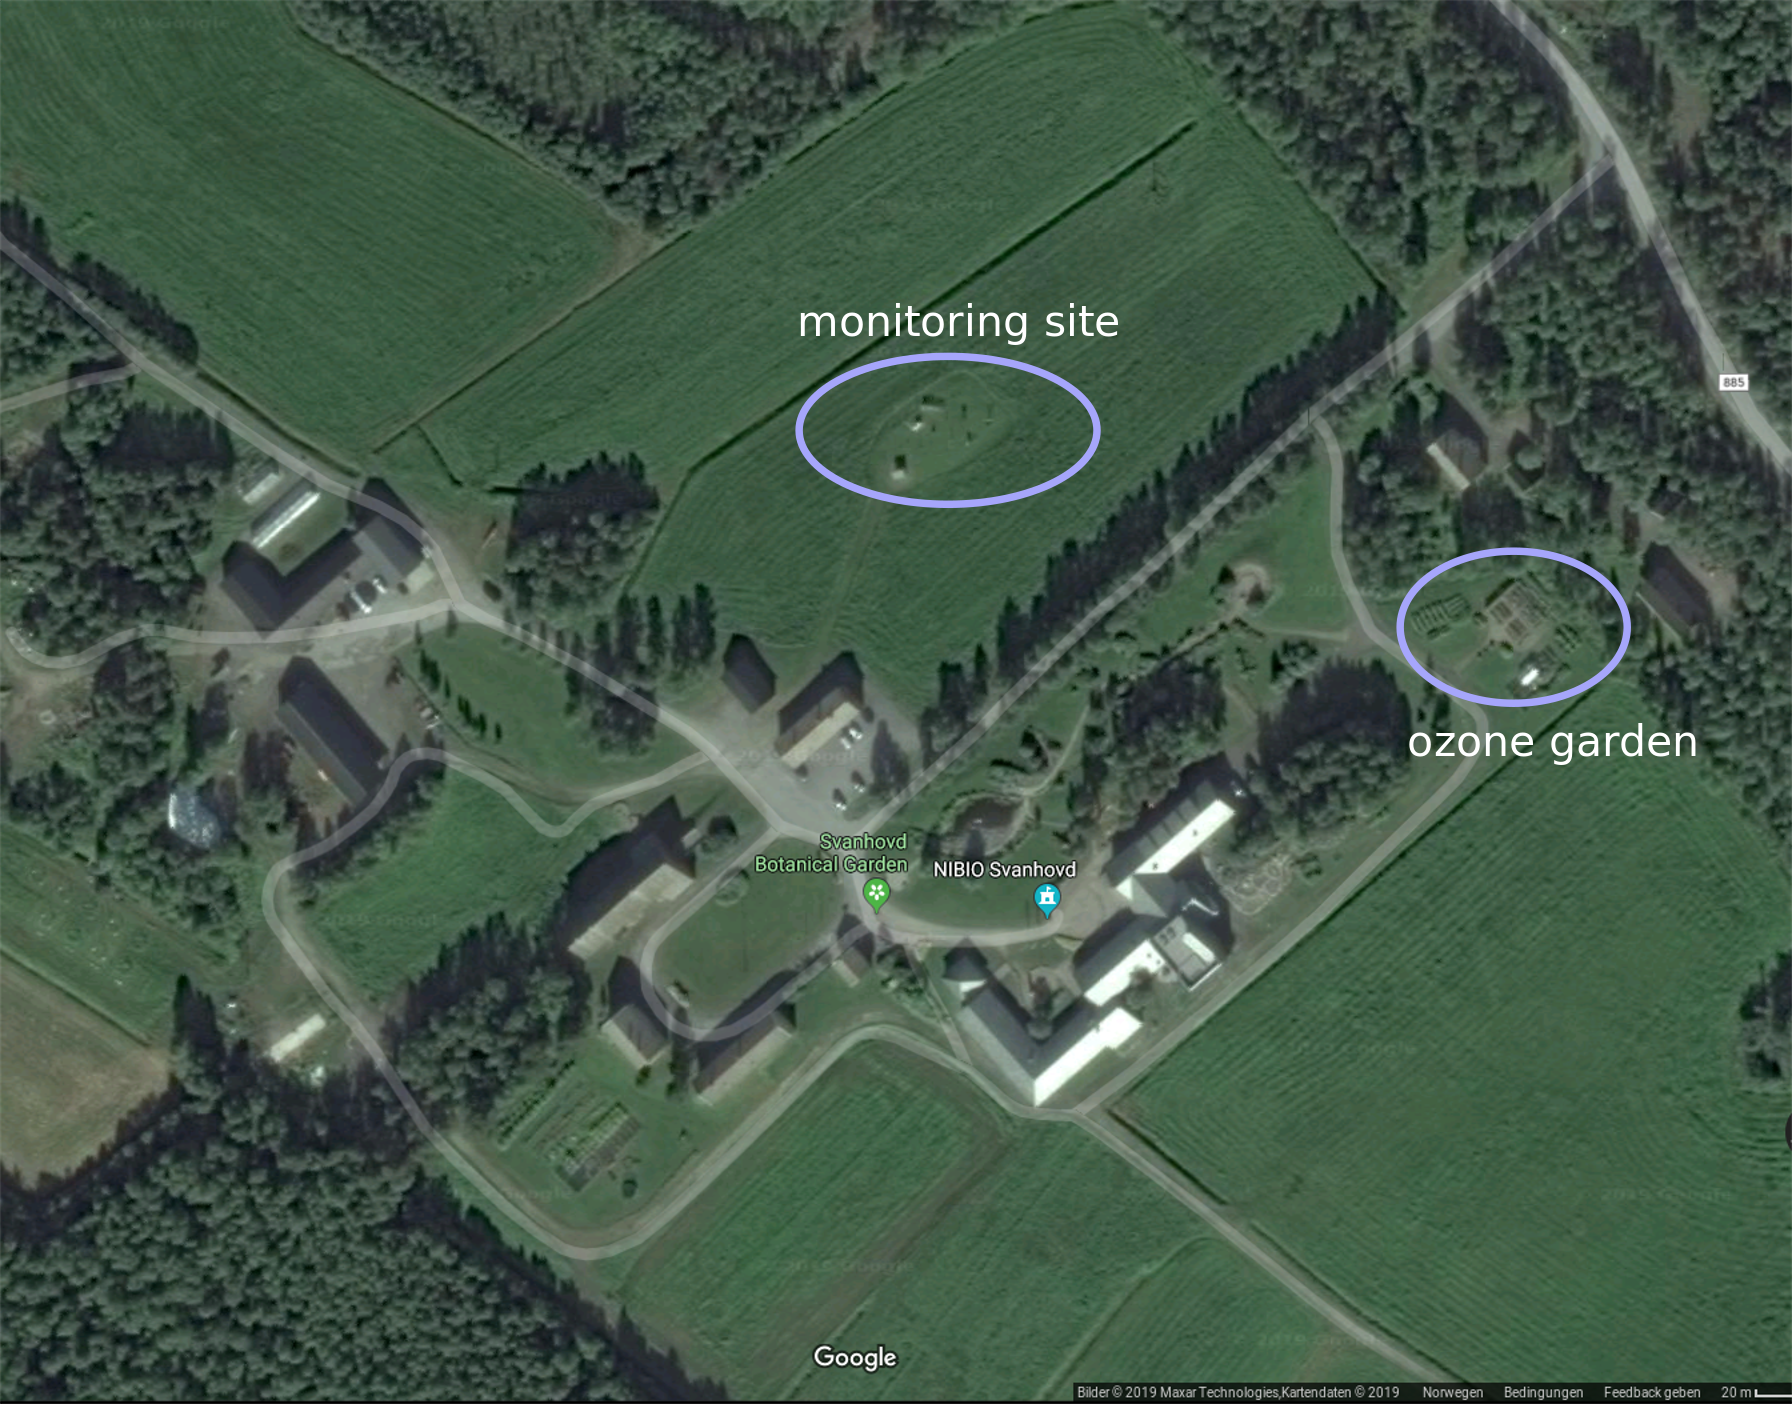
\includegraphics[width=8.3cm]{svanhovd_researchstation}
  \caption{NIBIO Environment Centre Svanhovd close by the settlement of Svanvik, Norway. Atmospheric monitoring site and ozone garden have been marked. Aerial photography \copyright Norges Kartverk.}
  \label{fig:svanhovd_research_station}
\end{figure}


\subsubsection{Atmospheric monitoring}
\label{subsubsec:atmo_svanvik}
For the growing seasons 2018/19, monitoring data of key variables (temperature, pressure, precipitation, and ozone) have been obtained from luftkvalitet.no which is operated by \citet{NILU_AIRQ}.

All agrometeorological variables including temperature and precipitation are available from September 1992 to present day \citep[LandbruksMeteorologiske Tjeneste][note the station name here is Pasvik]{LMT_NIBIO}.

Relevant data for the growing season 2018/19 are shown in Fig.~\ref{fig:data_svanvik_2018_2019}. The hatched areas mark times when no ozone data was recorded. Note, while the downtime during winter was planned, missing data in two weeks of July 2018 (July 9--23) were due to problems in data acquisition.

Ozone concentrations \chem{[O_3]} measured in $2\,\unit{m}$ height above ground are averaged hourly. As can be seen in Fig.~\ref{fig:data_svanvik_2018_2019}a), \chem{[O_3]} peaks in spring (April/May) and reaches its minimum in late summer (July/August). The spring peak has not been captured completely in 2019, for data acquisition started later than in 2018. In summer 2018 (June--August), high ozone concentrations ($\chem{[O_3]} > 40\,\unit{ppb}$) were recorded 50 times. The highest summer ozone concentration ($\chem{[O_3]} = 50.2\,\unit{ppb}$) was measured on July 25. This coincides with the period of the most extensive forest fires in central Sweden (G\"{a}vleborgs, J\"{a}mtlands, and Dalarnas l\"{a}n) which occurred from July 12--29 and destroyed about $18000\,\unit{hectare}$ of forest \citep{SOU2019}. However, due to the above mentioned data acquisition problems, we missed most of the corresponding ozone data for this event and most likely also the peak ozone concentration. In contrast, ozone concentration only rose 18 times above the threshold of $40\,\unit{ppb}$ during the summer of 2019.

Hourly averaged $2\,\unit{m}$ temperatures below $-20\,\unit{^\circ C}$ were observed in winter (January/February), while high temperatures (above $20\,\unit{^\circ C}$) occurred in summer (July), though more regularly in 2018 than in 2019 (Fig.~\ref{fig:data_svanvik_2018_2019}b). In 2018, temperature regularly rose above freezing only in May, while in 2019 this occurred already early in March/April. 2019 saw a very cold November with temperatures regularly below $-10\unit{^\circ C}$.

More rain events with accumulated daily precipitation $\sum_d \mathrm{Precip}$ above $10\,\unit{mm}$ occurred in the summer of 2018 compared to 2019 (Fig.~\ref{fig:data_svanvik_2018_2019}c). $\sum_d \mathrm{Precip} \ge 20\,\unit{mm}$ was only breached twice in 2018 and once in 2019.

In 2018, global irradiance $Q_0$ (Fig.~\ref{fig:data_svanvik_2018_2019}d) displays more sequentially high values in spring (May) and summer (July) compared to 2019, while June 2019 saw more consecutive high irradiance than 2018. In both years, the maximum recorded $Q_0$ was roughly $750\,\unit{W\,m^{-2}}$ reached only in June.

\begin{figure*}[t]
  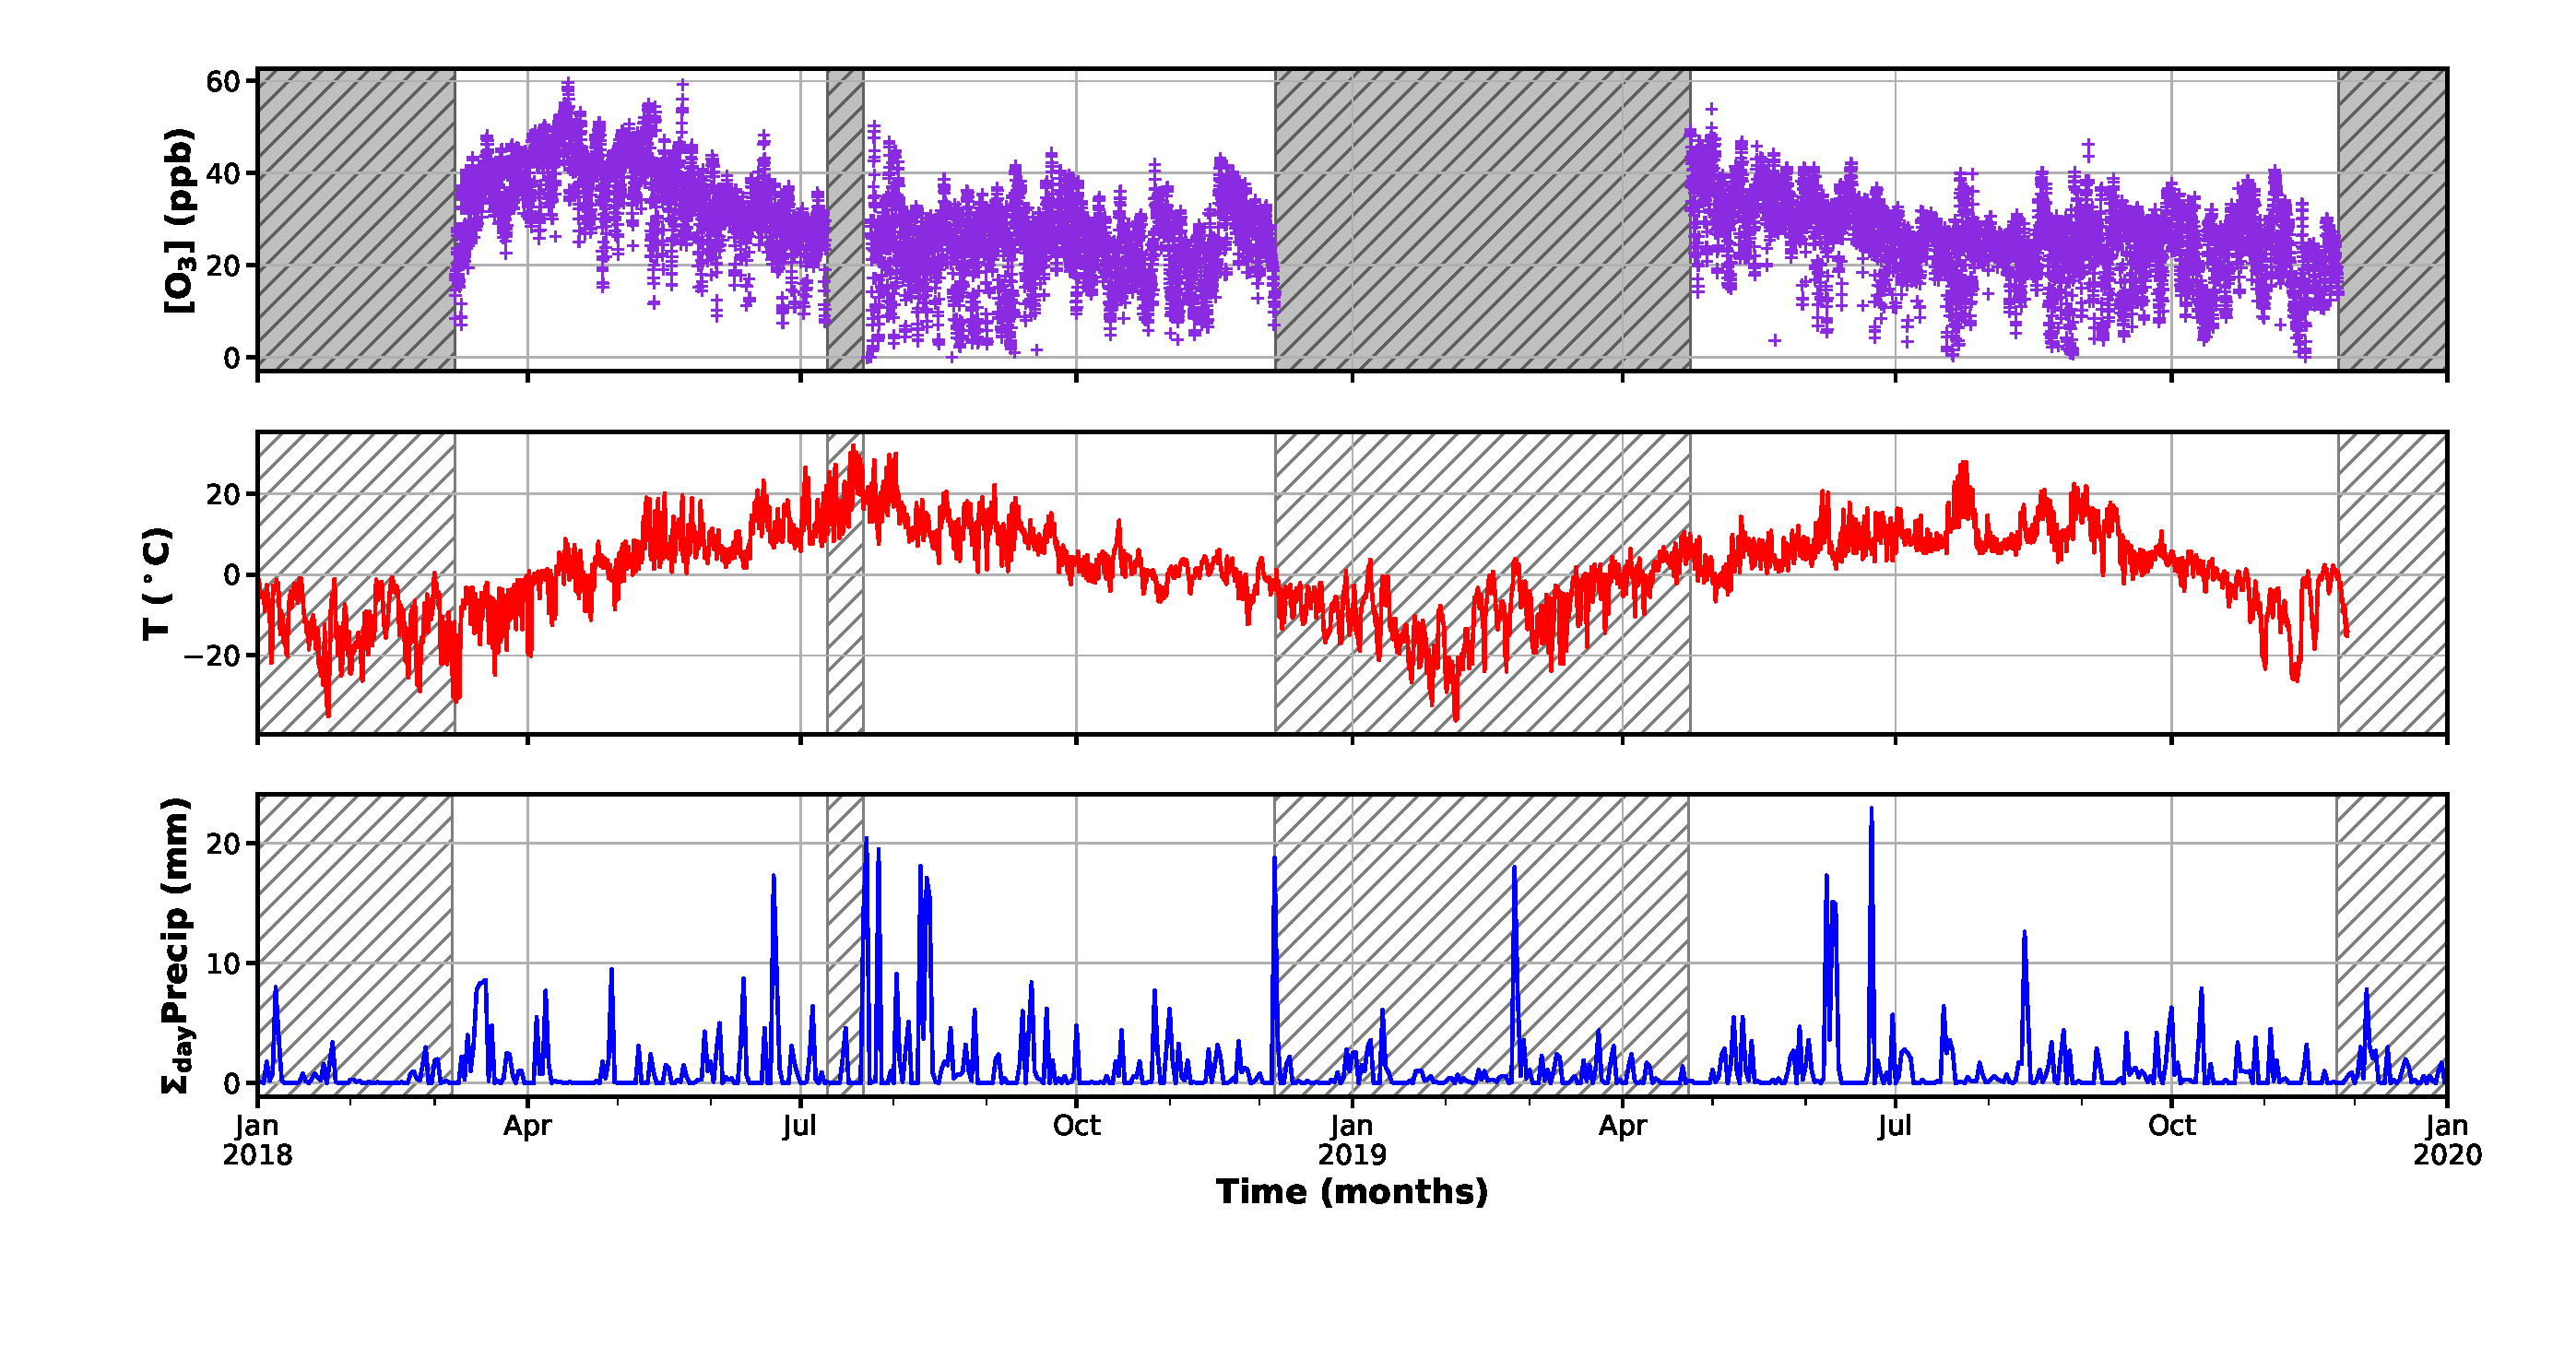
\includegraphics[width=12cm]{data_svanvik_2018_2019}
  \caption{Observational data from atmospheric monitoring at Svanhovd in 2018/19. The hatched areas indicate missing ozone monitoring data. (a) Hourly averaged ozone concentration; (b) hourly averaged temperature; (c) daily accumulated precipitation; (d) hourly averaged global irradiance.}
  \label{fig:data_svanvik_2018_2019}
\end{figure*}


\subsubsection{Ozone garden}
\label{subsubsec:ozone_garden}
An ozone garden consists of carefully selected plant species of which one cultivar is more sensitive to ozone than the other. At the NIBIO Environment Centre Svanhovd, the likely northern-most ozone garden to date, an ozone garden was installed in the course of our project. Cultivated species were, e.g. clover, tobacco, and beans. As shown in Fig.~\ref{fig:ozone_garden}, the plants had to be protected from herbivores with a wire-mesh fence. In 2018, we have observed ozone damage on semi-natural vegetation (clover) and crops (tobacco) in the ozone garden. In contrast, no such damage was found on the clovers in 2019, although it was found on the sensitive tobacco cultivar. This indicates that the vegetation may have been more affected by ozone in 2018 than in 2019.

\begin{figure}
  \includegraphics[width=8.3cm]{IMG_7739.JPG}
  \caption{Clover in the Svanhovd ozone garden. The plants had to be secured against herbivores with a wire-mesh fence. The plants shown are approximately $6-12\,\unit{cm}$ in height.}
  \label{fig:ozone_garden}
\end{figure}


\subsection{Other data}
\label{subsec:other_data}
To determine the significance of the ozone conditions in 2018, we have to derive a surface ozone concentration climatology for Svanvik. From 1986--1996 ozone monitoring has been operated by NILU at Svanhovd, but no ozone measurements have been conducted for the past $14\,\unit{years}$. Due to probable changes in northern hemispheric tropospheric background ozone and a reduction of summertime peak values related to ozone precursors which fell under air quality regulations in Europe, we also have to have a look at ozone observations at other sites in northern Fennoscandia. In regard to ozone, available observational data are sparse in this region. An overview over the geographical locations of conducted atmospheric monitoring in the past and present is given in Fig.~\ref{fig:station_map_fennoscandia}. The data is described in Section~\ref{subsubsec:ebas}. 
As additional complement to observational data which is not available at all times and spatially sparse, we also look at various ozone reanalysis products (Section~\ref{subsubsec:ozone_rea}).

\begin{figure}[t]
  \includegraphics[width=8.3cm]{station_map_fennoscandia}
  \caption{Cap of the North. Locations of past and present ozone observation sites in northern Fennoscandia used within this study. For more details see Tab.~\ref{tab:ebas_obs}. The same color coding for each station as displayed herein will be used in all following figures.}
  \label{fig:station_map_fennoscandia}
\end{figure}

\subsubsection{Surface ozone observations}
\label{subsubsec:ebas}
All surface ozone observations used in this study are available from the EBAS database operated by \citet{NILU_EBAS}. In Table~\ref{tab:ebas_obs}, we give an overview over the exact locations and time range of operational data taking. All stations with available long term observations are located on higher ground than Svanhovd which will result in higher surface ozone concentrations in comparison as ozone abundance, in general, decreases with decreasing altitude in the absence of local precursors \citep[e.g.,][]{AB:Klingberg2009}. The periphery vegetation at all sites is similar and consists mainly of pine forests, birch, and heath. However, at close vicinity it varies substantially. Ozone measurements at Pallas are taken on top of mount Sammaltunturi $100\,\unit{m}$ above tree line (pine forest) and mainly consists of low vascular plants, mosses, and lichen \citep{BER:Hatakka2003}. At Svanhovd, the ozone measurements are taken amidst a meadow surrounded by agriculturally managed herbaceous plants and grass (c.c. Fig.\ref{fig:svanhovd_research_station}).

Data from before the 1990s is available solely from Svanvik and Karasjok. These data, however, do not follow the high quality standard procedures implemented nowadays and have to be treated with care \citep{NILU2003}. Especially, ozone monitors did not undergo a regular re-calibration. This probably leads to drifts in the observed data and may impose a false periodicity. In 1997, the ozone monitoring at Jergul was relocated downstream the river Karasjokka to a site close by Karasjok. Although the same equipment has been used, this might have introduced a breaking point in the combined data series, denoted as Jergul/Karasjok in the following, which would be of a problem if this was the sole data to compare with. Only few data have been taken upstream the Pasvik river at Janiskovski, hence these will not be taken into further consideration, but are shown for completion. As can be seen in Fig.~\ref{fig:ozone_timesseries_fenoscandic_obs}, there is an overlap of about $4\,\unit{years}$ between data taken at Esrange, Jergul/Karasjok, and Svanvik. The hatched areas indicate time periods with insufficient quality control as mentioned above.

\begin{table}[t]
  \caption{Past and present ozone observation sites in northern Fennoscandia. Data available on \href{http://ebas.nilu.no/}{EBAS}.}
  \label{tab:ebas_obs}
  \begin{tabular}{lllllrl}
    \tophline
    Name       & Country & ID      & \multicolumn{3}{c}{Location} & Operational\\
    &         &         & lat             & lon               & alt            &\\
    &         &         & (\unit{^\circ N}) & (\unit{^\circ E})  & (\unit{m})     &\\
    \middlehline
    Esrange    & SWE     & SE0013R & 67.83           & 21.07             & 475            & 1991 -- present\\
    Janiskoski & RUS     & RU0001R & 68.93           & 28.85             & 118            & 1995 -- 1997\\
    Jergul     & NOR     & NO0030R & 69.45           & 24.60             & 255            & 1997 -- 2011\\
    Karasjok   & NOR     & NO0055R & 69.467          & 25.217            & 333            & 1988 -- 1997\\
    Pallas     & FIN     & FI0096G & 67.97           & 24.12             & 565            & 1995 -- present\\
    Svanvik    & NOR     & NO0047R & 69.45           & 30.03             & 30             & 1986 -- 1996$^\dagger$\\
    \bottomhline
  \end{tabular}
  \belowtable{$^\dagger$ Exclusive ozone monitoring growing seasons 2018/19 operated by NILU.} % Table Footnotes
\end{table}


\begin{figure*}[t]
  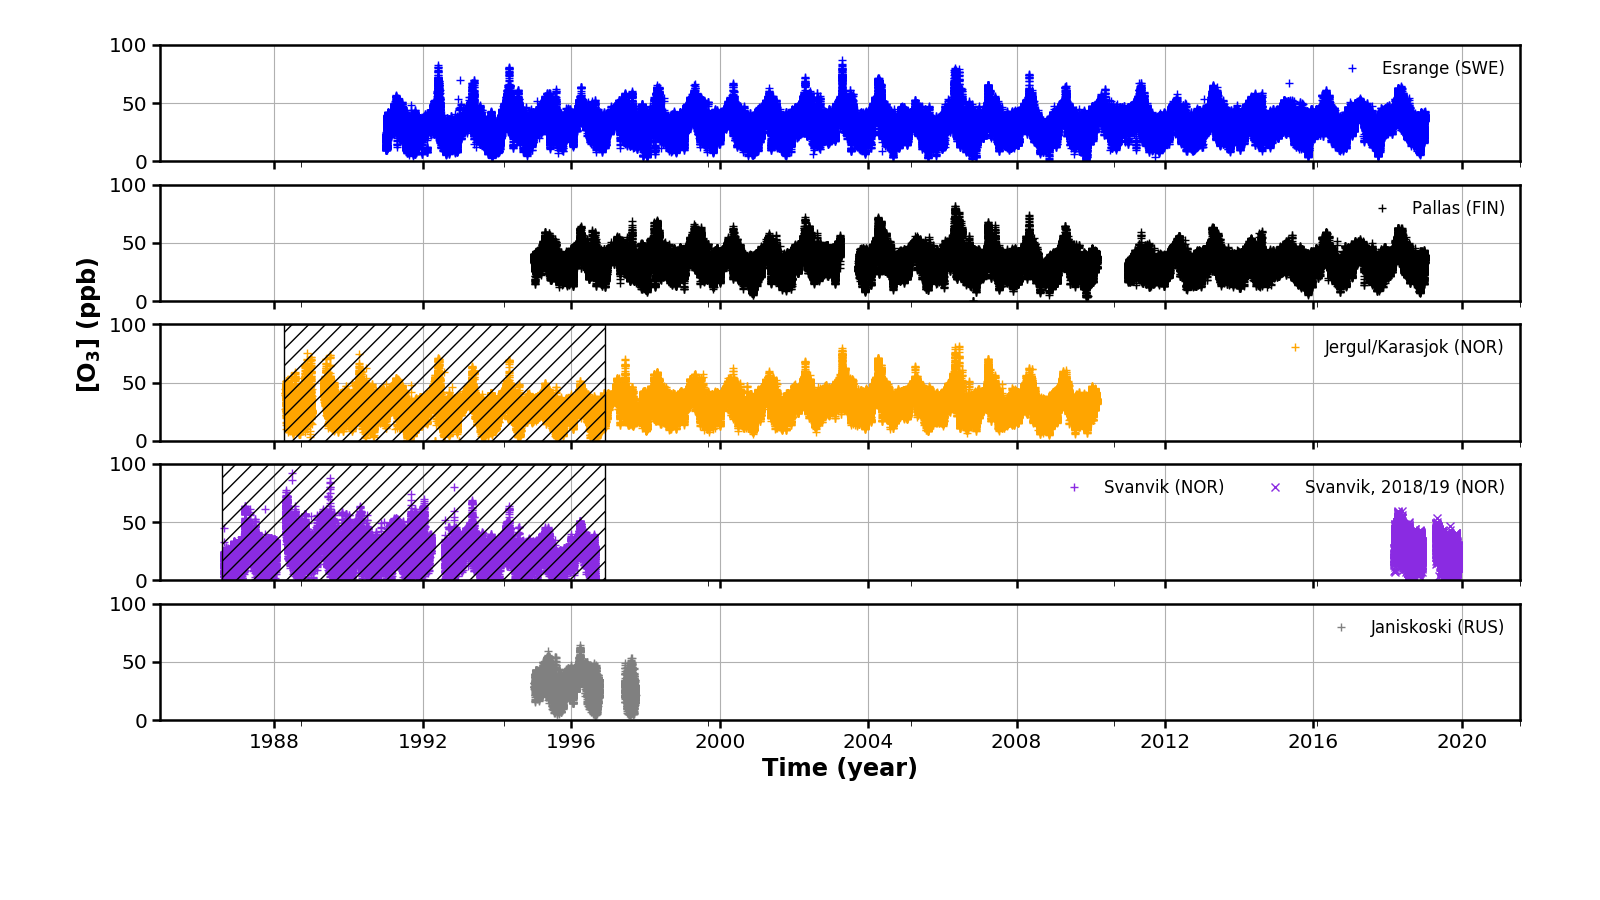
\includegraphics[width=12cm]{ozone_timeseries_fenoscandic_obs.png}
  \caption{Time series of ozone observations in northern Fennoscandia (Tab.~\ref{tab:ebas_obs}). Data taken from EBAS. The hatched areas indicate time periods with insufficient quality control \citep{NILU2003}.}
  \label{fig:ozone_timesseries_fenoscandic_obs}
\end{figure*}

\subsubsection{Ozone reanalysis}
\label{subsubsec:ozone_rea}

Details of reanalysis data sets referred to in this work are listed in Table~\ref{tab:ozone_rea}.
There are two global reanalysis products available at the European Centre for Medium-Range Weather Forecasts (ECMWF) that include atmospheric tracers, in particular ozone (MACC and CAMSRA) \citep{ACP:Inness2013, ACP:Inness2019}. The temporal as well as spatial resolution of these reanalysis products is rather coarse: 3-hourly and $0.75^\circ\times 0.75^\circ$ or roughly $29.3\,\unit{km}\times 83.4\,\unit{km}$ at the location of Svanvik, respectively. In addition, higher resolution surface ozone reanalysis for whole Europe is available from Copernicus service for regional air quality control (note: since May 31st 2020 through the CAMS Atmosphere Data Store (ADS)). The regional air quality model reanalysis ensemble (CAMS regional Ensemble) is based on nine European state-of-the-art numerical air quality models \citep{Copernicus_Regio_AIRQ}. The ensemble mean is at fairly high spatial and temporal resolution compared to the global reanalysis from ECMWF: $0.1^\circ\times 0.1^\circ$ or roughly $3.9\,\unit{km}\times 11.1\,\unit{km}$ and 1-hourly, respectively. The covered time periods differ and no data are available for before the turn of the millennium. The CAMSRA and CAMS Regional Air Quality ensemble mean are available in near real time, but only former covers a period of sufficient length for climate analysis (2003 -- present). All reanalyses use different but, at that time, latest versions of the operational weather forecast system (OpenIFS) from ECMWF. They differ substantially in the assimilated observational ozone data. The MACC reanalysis assimilates only satellite derived tropospheric column ozone (TC), while CAMSRA also includes ozone profiles from satellite retrievals. Most importantly for our study, in situ observations from ozone surface station networks are only assimilated in the CAMS Regional Ensemble. The quality with respect to observations in northern Fennoscandia will be discussed in Section~\ref{subsubsec:clim_ozone}. Without too much foreshadowing, the results prevented us from fetching the whole CAMSRA data.

\begin{table}[t]
  \caption{Ozone related reanalysis products used in this study: \href{https://www.ecmwf.int/en/newsletter/158/meteorology/new-cams-global-reanalysis-atmospheric-composition}{Global reanalysis (ECMWF)}; \href{https://www.regional.atmosphere.copernicus.eu/}{ensemble mean of regional reanalysis for Europe (Copernicus)}.}
  \label{tab:ozone_rea}
\begin{tabular}{llcclcc}
\tophline
Name & Provider & \multicolumn{2}{c}{Resolution} & Time period & Meteorological forcing & \chem{O_3} assimilation\\
&              & spatial & temporal & & \\
\middlehline
MACC & ECMWF & $0.75^\circ \times 0.75^\circ$ & 3-hourly & 2003 -- 2012 & OPS & satellite $^\triangledown$\\
CAMSRA & ECMWF & $0.75^\circ \times 0.75^\circ$ & 3-hourly & 2003 -- 2012 $^\dagger$ & ERA5 / OPS $^\ddagger$ & satellite $^\blacktriangledown$\\
CAMS Regional Ensemble & Copernicus & $0.1^\circ \times 0.1^\circ$ & 1-hourly & 2014 -- 2018 $^\dagger$ & OPS $^\star$ & in situ $^\vartriangle$\\
\bottomhline
\end{tabular}
\belowtable{$^\dagger$ Subset of the data used in this study. The full data set extends into near real time; $^\ddagger$ ERA5 (2003--2016), OPS (later); $^\star$ EURAD uses WRF for downscaling of operational IFS; $^\triangledown$ MLS, OMI - tropospheric column; $^\blacktriangledown$ SCIAMACHY, MIPAS, MLS, OMI, GOME2, SBUV2 - tropospheric column + profile; $^\vartriangle$ METEO France NRT.} % Table Footnotes
\end{table}


\section{Statistical analysis of environmental key variables}
\label{sec:stats}
In this section, we will evaluate atmospheric conditions in the growing seasons of 2018/19 by statistical means. We will derive climatologies for both, temperature, precipitation, global irradiance, and ozone for Svanvik (Section~\ref{subsec:climatologies}). The ozone measurements will be put into a climatological as well as regional context. We will look at anomalies of the atmospheric key variable mentioned above (Section~\ref{subsec:anomalies}).

\subsection{Derived climatologies}
\label{subsec:climatologies}

\subsubsection{Temperature, precipitation, and global irradiance}
\label{subsubsec:clim_temp_prec}
The location of Svanvik at $69.45\,\unit{^\circ N}$ suggests a subarctic climate. The derived climate diagram following Walter and Lieth shown in Fig.~\ref{fig:climatediagram} supports this very well. The diagram is based on climatological data from Svanvik (1992--2012) downloaded from LandbruksMeteorologiske Tjeneste. Monthly averaged temperatures (red line) are displayed with standard error of mean as error band. Averaged monthly accumulated precipitation (blue bars) is shown with standard deviation of mean as error bars. Months with average temperatures below freezing are denoted with a star. As can be seen, temperatures stay below freezing for 5 consecutive months, while only 2 months breach $10\,\unit{^\circ C}$ regularly (July, August), satisfying the conditions for K\"{o}ppens climate classification of a regular subarctic climate (Dfc). The highest monthly average temperature is $(13.1\pm 1.1)\,\unit{^\circ C}$ in July and the lowest $(-12.8\pm 2.0)\,\unit{^\circ C}$ in February. In the time period 1992--2012, the coldest measured temperature was $-45.2\,\unit{^\circ C}$ observed January 27, 1999, while the highest temperature on July 16 the same year was $29.4\,\unit{^\circ C}$.

Winter and spring (November--April, except for March) are relatively dry ($\sum_m \mathrm{Precip} < 20\,\unit{mm}$). The driest month is January with $\sum_m \mathrm{Precip} = (16.7\pm 3.0)\,\unit{mm}$. The most precipitation occurs in the summer months, with a highest monthly averaged accumulated precipitation $\sum_m \mathrm{Precip} = (58.5\pm 9.2)\,\unit{mm}$ in August. The average annual accumulated precipitation given with standard error of mean is $(383\pm 86)\,\unit{mm}$. Precipitation shows a large variability throughout the years.

A climatology derived for global irradiance $Q_0$ is shown in Appendix Fig.~\ref{fig:global_rad_clim}a) for both, climatological average of hourly maximum $\left<Q_0^\mathrm{max}\right>$, minimum $\left<Q_0^\mathrm{min}\right>$, and mean $\left<Q_0^\mathrm{mean}\right>$ irradiance observed at Svanvik. In agreement with the geometrically derived sunshine duration shown in Appendix Fig.~\ref{fig:sunlight_fennoscandia}, $\left<Q_0^\mathrm{max}\right>$ approaches zero in December/January commonly known as polar night and reaches its maximum in June/July commonly referred to as midnight sun conditions. The highest observed $\left<Q_0^\mathrm{max}\right>$ is about $800\,\unit{W\,m^{-2}}$, while on average $\left<Q_0^\mathrm{mean}\right>$ it is about $450\,\unit{W\,m^{-2}}$ (regularly reached in May--July). The maximum of the climatological minimum $\left<Q_0^\mathrm{min}\right>$ lies at about $200\,\unit{W\,m^{-2}}$.

\begin{figure}[t]
  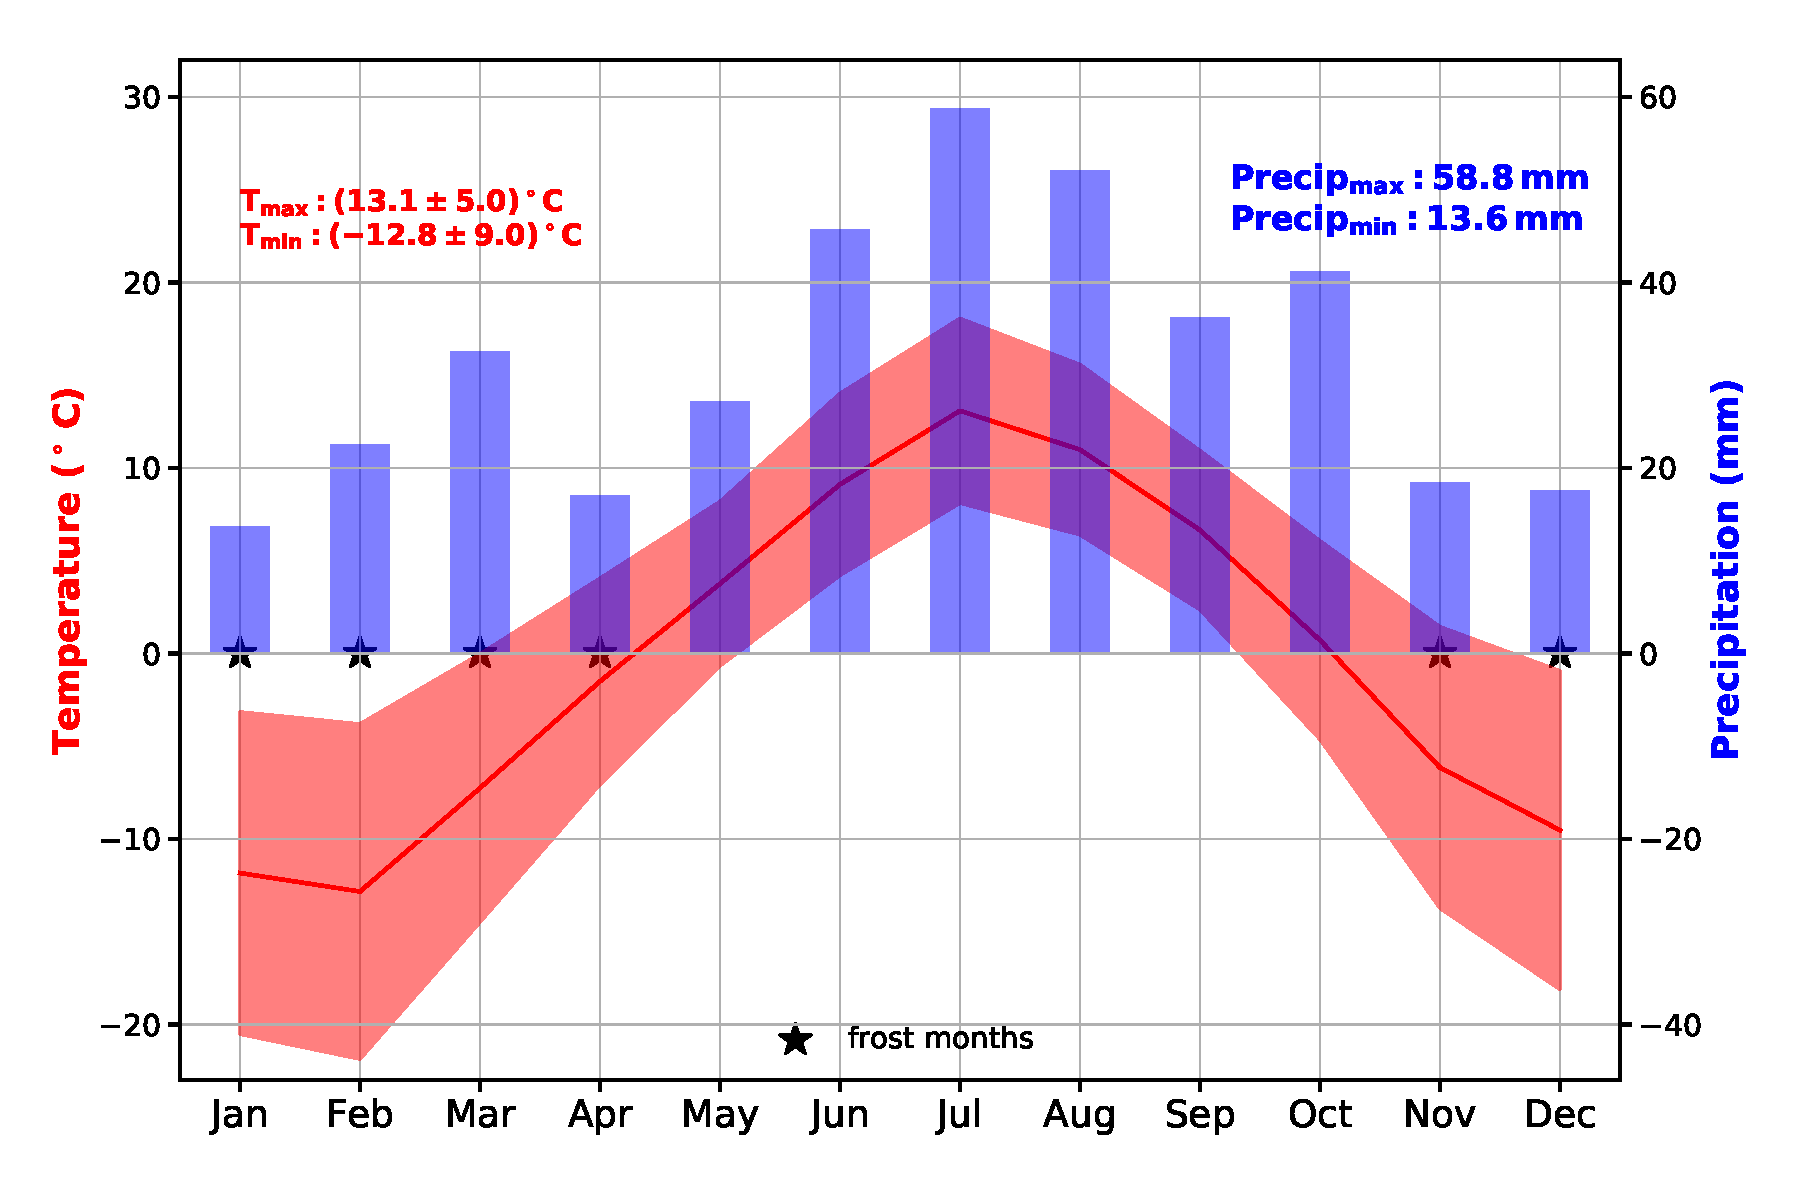
\includegraphics[width=8.3cm]{climatediagram}
  \caption{Climate diagram following Walter and Lieth. The diagram is based on climatological data for Svanvik/Pasvik (1992--2012) downloaded from LandbruksMeteorologiske Tjeneste. Monthly averaged temperatures (red line) are displayed with standard error of mean as error band. Averaged monthly accumulated precipitation (blue bars) is shown with standard deviation of mean as error bars. Months with average temperatures below freezing are denoted with a star.}
  \label{fig:climatediagram}
\end{figure}

\subsubsection{Ozone}
\label{subsubsec:clim_ozone}
In the following, we will look at derived ozone climatologies from different perspectives.
The multi-annual means of daily mean ozone, for simplicity here without standard deviations, at observation sites in northern Fennoscandia (refer to Table~\ref{tab:ebas_obs} for details) are shown in Fig.~\ref{fig:ozone_climatology_fenoscandic_obs}. All climatologies peak in spring, with peak values of about $48\,\unit{ppb}$ in late April. The annual average ozone concentration \chem{\left<[O_3]\right>} declines throughout the growing season until it reaches its minimum in late summer/fall ($24-30\,\unit{ppb}$). The turning points lie approximately in June and November. The ozone climatology lags about 3 months behind the temperature climatology. At Svanvik, \chem{\left<[O_3]\right>} is $6.6\,\unit{ppb}$ lower than on sites at Jergul/Karasjok (NOR), Esrange (SWE), and Pallas (FIN). The large spread in case of Svanvik and Janiskoski can be explained due to the lower overall statistics.

\begin{figure}[t]
  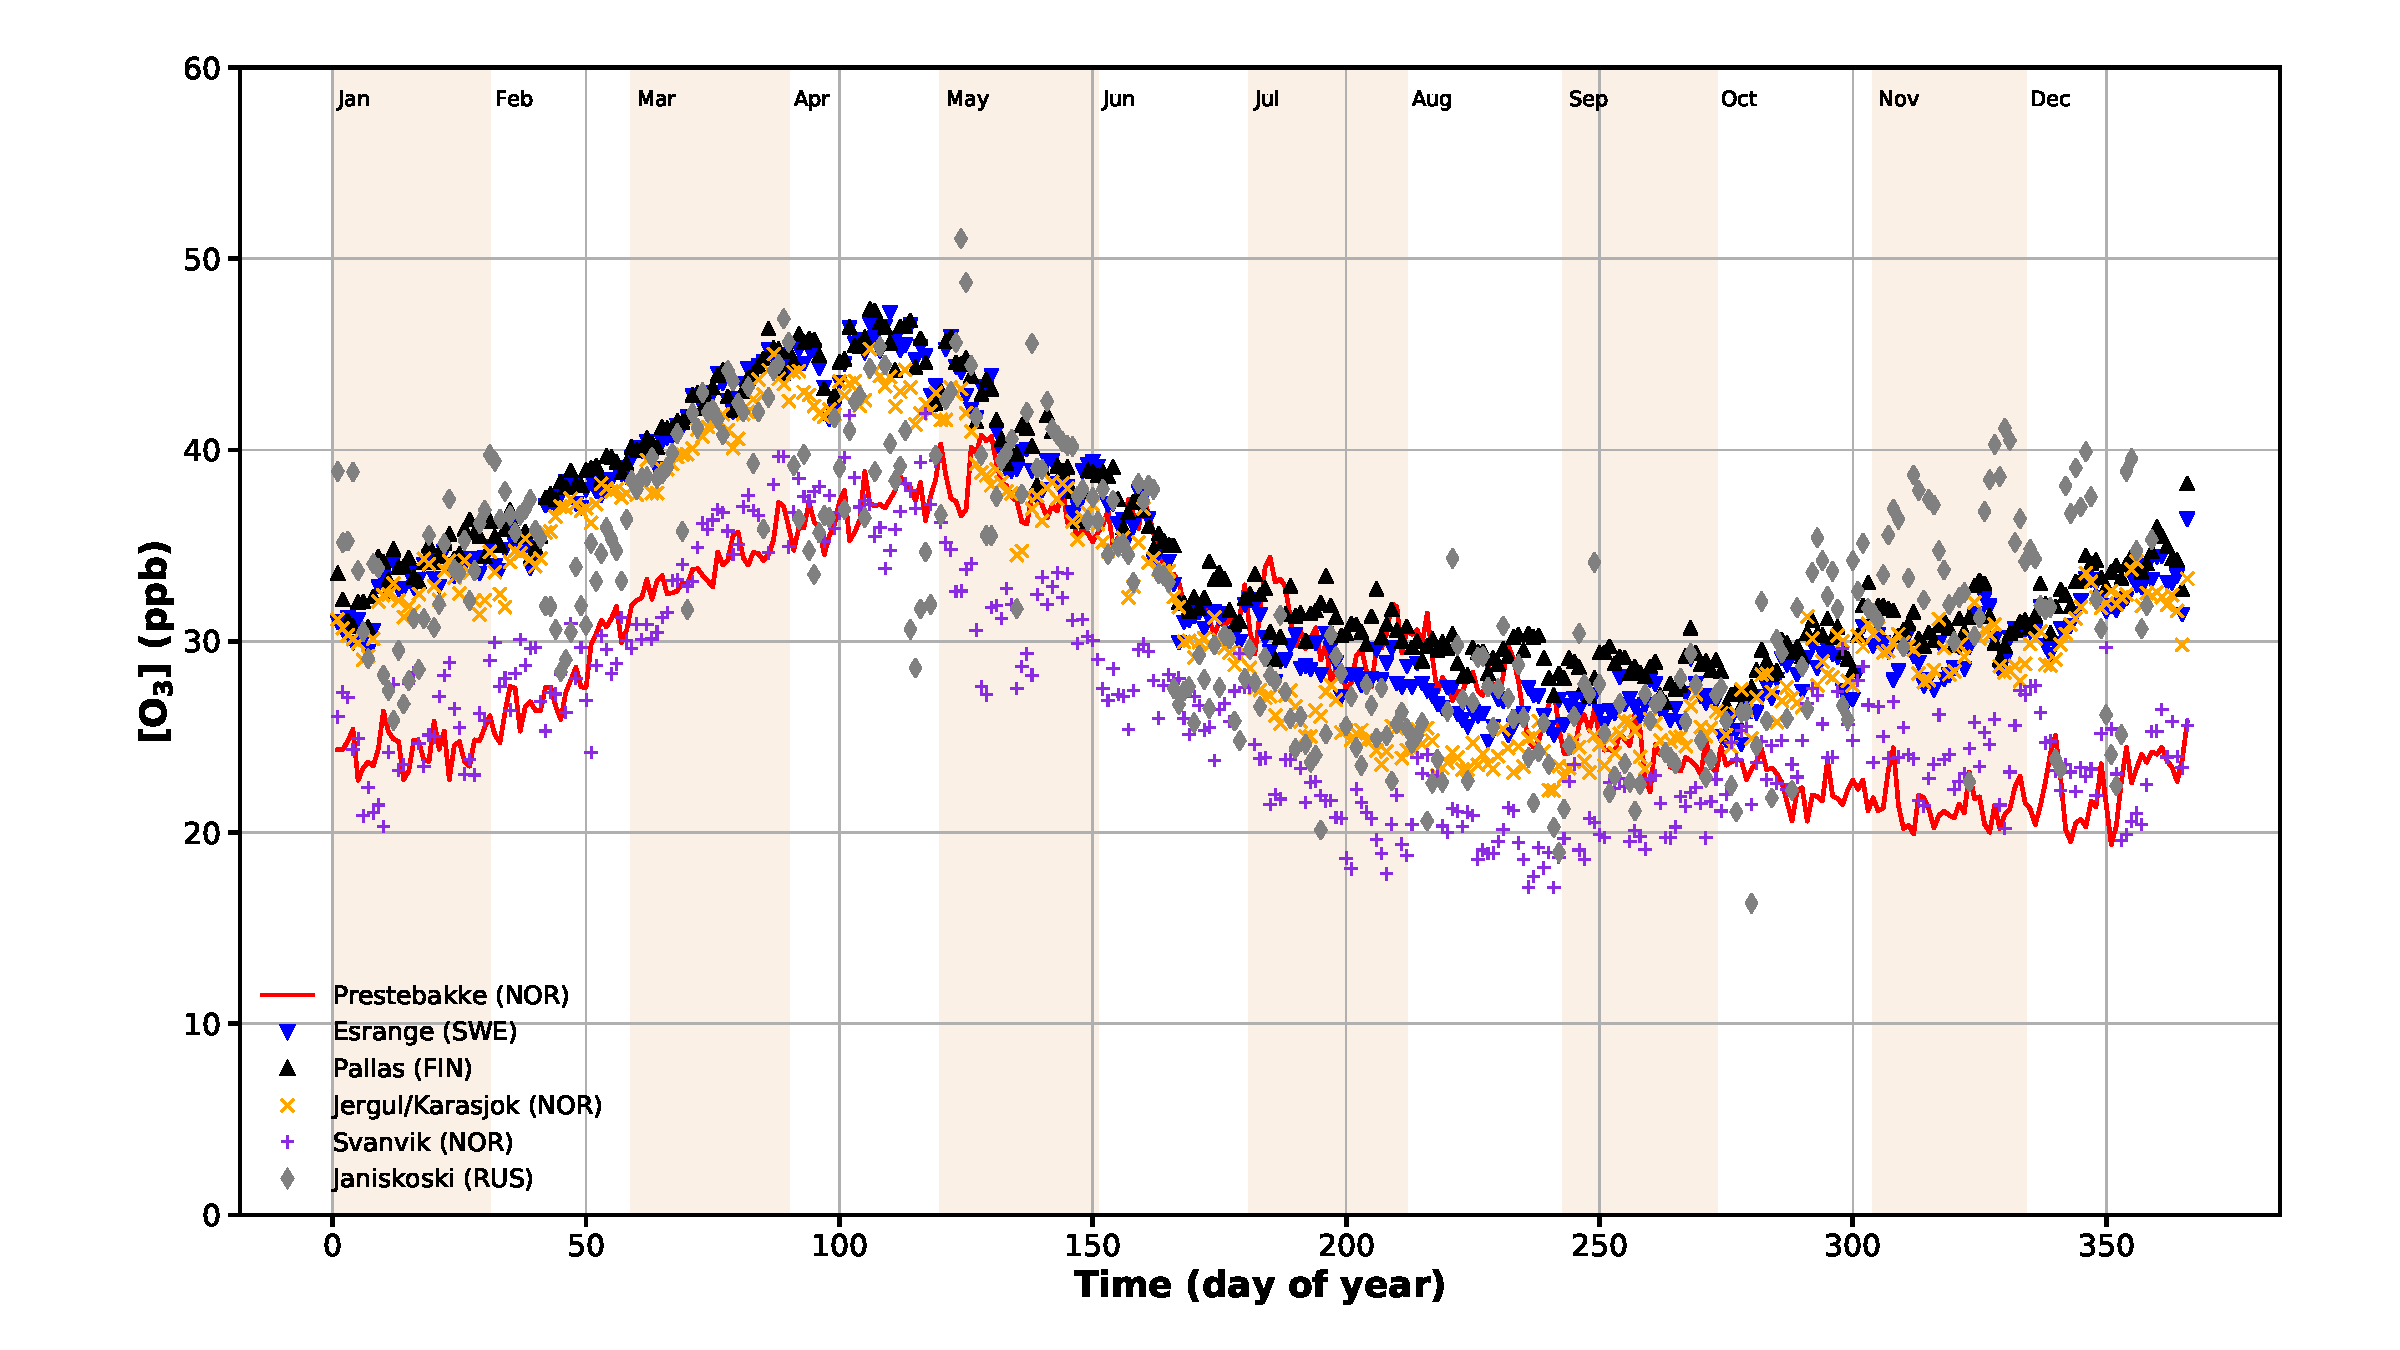
\includegraphics[width=8.3cm]{ozone_climatology_fenoscandic_obs}
  \caption{Multi-annual mean of daily mean ozone at observation sites in Fennoscandia. The large spread in case of Svanvik and Janiskoski is due to the lower statistics. All climatologies peak in spring, with peak values in April. The annual average ozone concentration \chem{\left<[O_3]\right>} at Svanvik is $6.6\,\unit{ppb}$ lower than at the sites at Jergul/Karasjok (NOR), Esrange (SWE), and Pallas (FIN).}
  \label{fig:ozone_climatology_fenoscandic_obs}
\end{figure}

The correlation of \chem{[O_3]} between Esrange, Pallas, and Jergul/Karasjok is fairly high ($r^2\approx 0.8$, Appendix Fig.~\ref{fig:density_distribution}a, b), hence we can put those data series together to derive a general ozone climatology for northern Fennoscandia. The correlation between Svanvik and Esrange and Pallas is rather low, 0.4 and 0.6, respectively. Thus, Svanvik cannot directly be represented by any measurements taken at either Esrange or Pallas. We shall come back to this in Section~\ref{subsec:ozone_reco}.

In Figure~\ref{fig:ozone_climatology_fenoscandic_obs_spline}, the 2 dimensional density distributions for the thus defined northern Fennoscandia (Fig.~\ref{fig:ozone_climatology_fenoscandic_obs_spline}a) and Svanvik (Fig.~\ref{fig:ozone_climatology_fenoscandic_obs_spline}b) are shown. Darker colors indicate higher probability to observe these values. On top of the density distributions, $10\,\unit{days}$ averages of daily mean \chem{\left<[O_3]\right>_\mathrm{10\,\unit{d}, mean}}, daily maximum \chem{\left<[O_3]\right>_\mathrm{10\,\unit{d}, max}}, and daily minimum \chem{\left<[O_3]\right>_\mathrm{10\,\unit{d}, min}} are displayed together with the $1 \sigma$ uncertainties, respectively. In addition, \chem{\left<[O_3]\right>_\mathrm{10\,\unit{d}, mean}} is also shown with standard error of mean (albeit small and hardly visible). Splines have been fitted through the data for easier inter-comparison with reanalysis data.

From the northern Fennoscandic climatology, one can deduce several features. The maximum of \chem{\left<[O_3]\right>_\mathrm{10\,\unit{d}, min}} peaks about $20\,\unit{days}$ earlier than the \chem{\left<[O_3]\right>_\mathrm{10\,\unit{d}, mean}}, and \chem{\left<[O_3]\right>_\mathrm{10\,\unit{d}, max}}. With respect to the periodicity of \chem{\left<[O_3]\right>_\mathrm{10\,\unit{d}, mean}}, it takes about $7.5\,\unit{months}$ from minimum concentration to maximum concentration, while from maximum to minimum it only takes about $4.5\,\unit{months}$. The maximum of \chem{\left<[O_3]\right>_\mathrm{10\,\unit{d}, max}} is at $52\,\unit{ppb}$ in late April and the minimum of \chem{\left<[O_3]\right>_\mathrm{10\,\unit{d}, min}} occurs at $15\,\unit{ppb}$ in the beginning of September. The steep rise of \chem{\left<[O_3]\right>_\mathrm{10\,\unit{d}, mean}} in spring is in coincidence with increasing temperatures as well as increase in global irradiance. The decrease in \chem{\left<[O_3]\right>_\mathrm{10\,\unit{d}, mean}} begins about one month ahead of the estimated onset of the greening season. Based on data from SeNorge.no and the agricultural rule of thumb that the daily average temperature has to be above $5\,\unit{^\circ C}$ for $5\,\unit{days}$ consecutively, we find $\left<G_\mathrm{begin}\right> = (150 \pm 14)\,\unit{days of the year}$ at Svanvik (Appendix Fig~\ref{fig:greening_season_change_Svanvik}), which translates into the end of May. This finding is in line with more extensive studies \citep[][e.g.,]{IJB:Karlsen2007,AFM:Linderholm}.

The density distribution for Svanvik and the respective \chem{\left<[O_3]\right>_\mathrm{10\,\unit{d}, mean}}, and \chem{\left<[O_3]\right>_\mathrm{10\,\unit{d}, max}} (Fig.~\ref{fig:ozone_climatology_fenoscandic_obs_spline}b) display a similar pattern as the northern Fennoscandic climatology. The spring peak apparently occurs slightly earlier (in the beginning of April). As Svanvik is located at lower altitude than the other sites, the earlier ozone peak may point to an interplay with ozone uptake by vegetation. {\bf TODO: The data from SeNorge seems to point to a later onset of greening, than what I interfered from OpenIFS data. This means that the beginning of the growing season is not a good measure for the termination of the ozone spring peak. This does not exclude the early start of pine forest photosynthesis as a driver. Coniferous forest starts to photosynthesis earlier than what the growing season begin would mark. \chem{CO_2} uptake and phenology of coniferous trees \citep{TB:Kolari2007} starts as early as doy 100, acclimates to leaf temperature history - photosynthesis drops at around doy 200--250.} The average ozone concentration at Svanvik is lower than at the other sites, as already mentioned, which is in league with a decrease in tropospheric ozone with decreasing altitude. In July--September, ozone is occasionally almost completely depleted during night time.

\begin{figure}[t]
  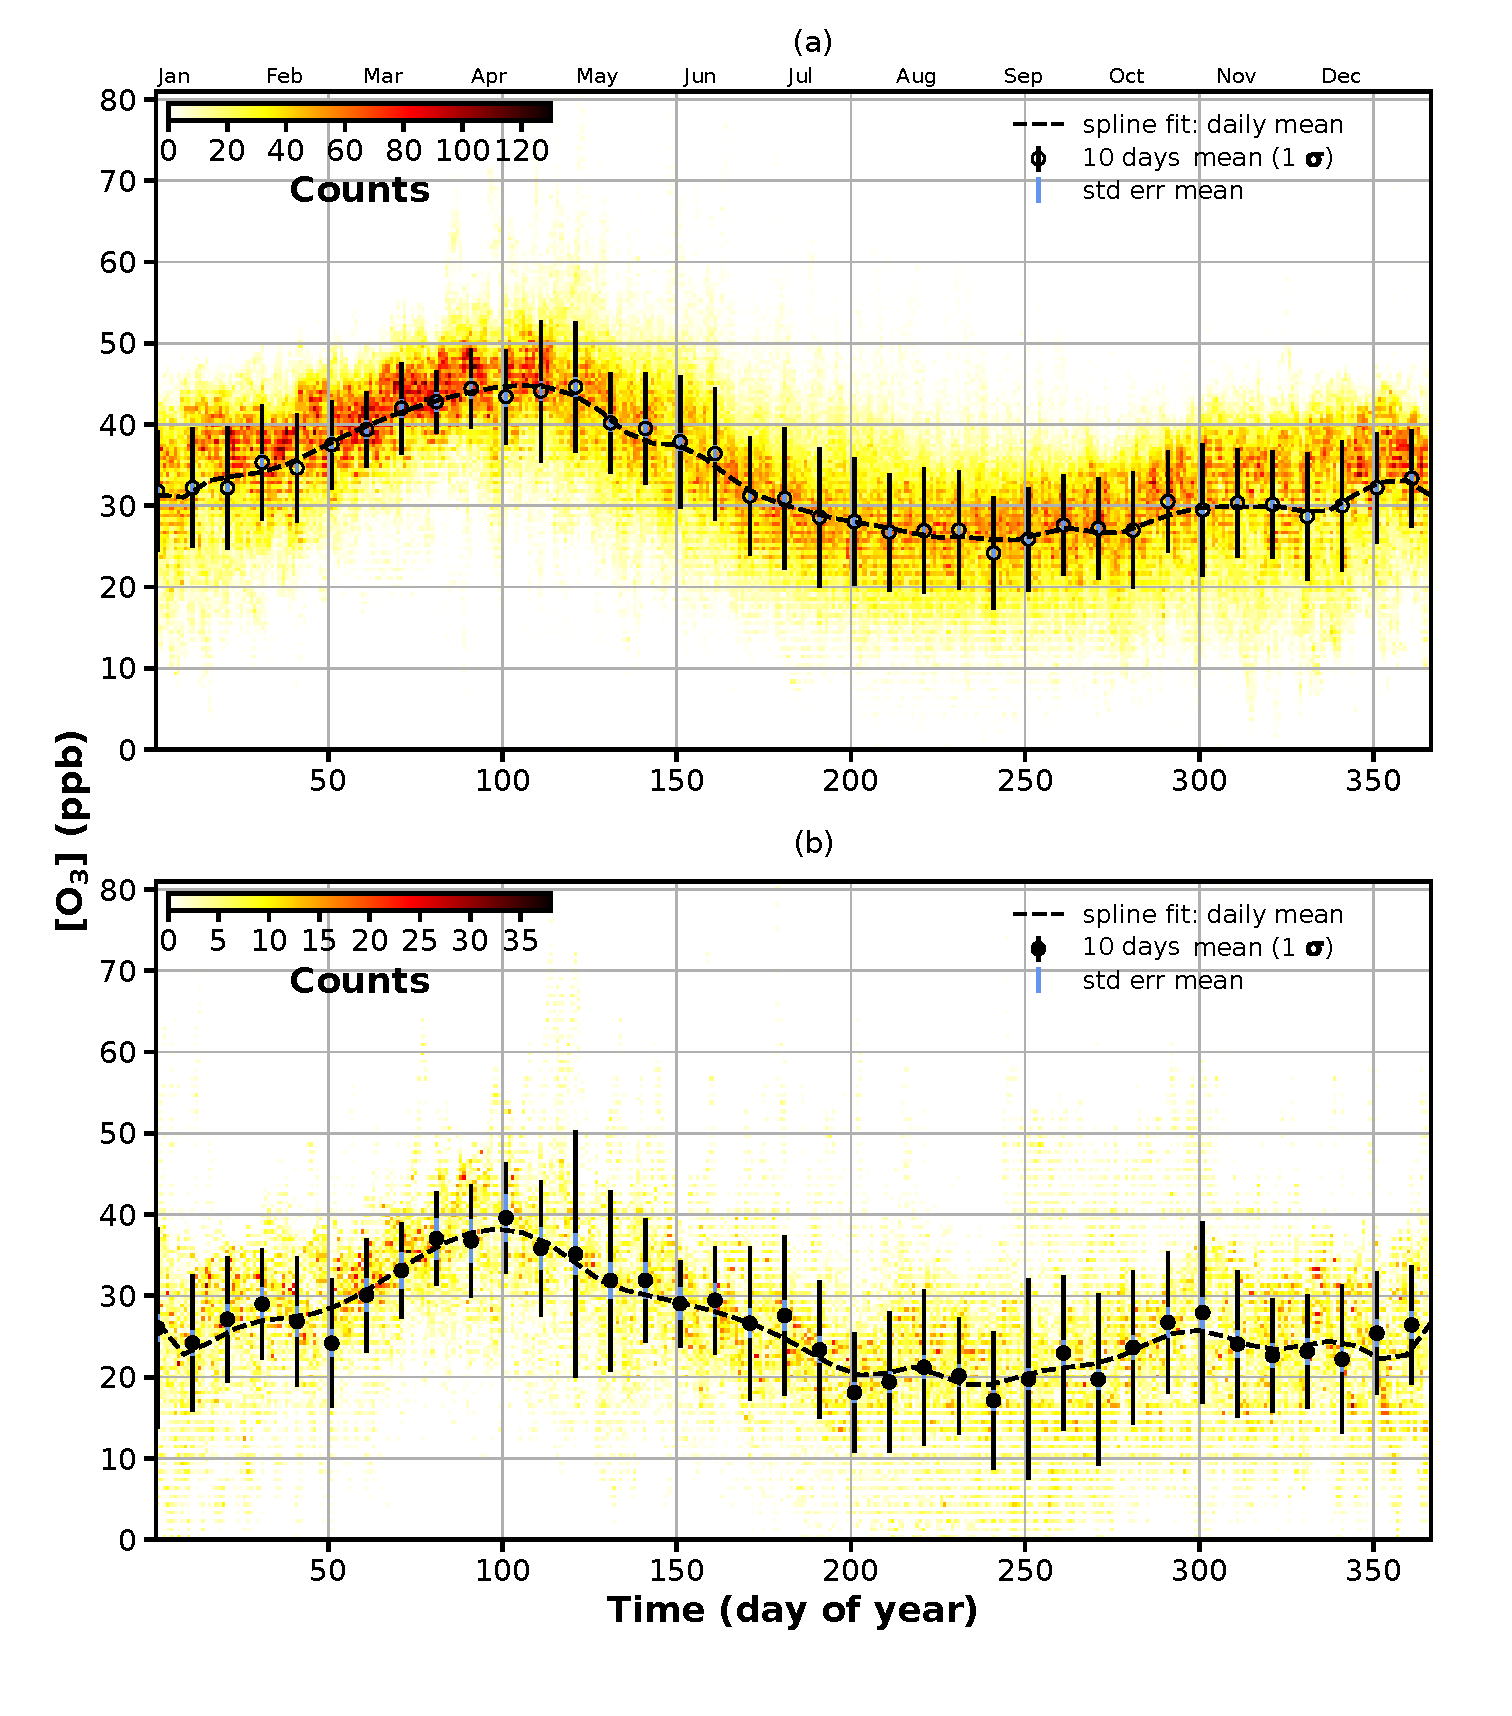
\includegraphics[width=8.3cm]{ozone_climatology_fenoscandic_obs_spline}
  \caption{Derivation of ozone climatologies. Density distributions are shown together with multi-annual mean of daily ozone concentrations \chem{[O_3]}. Splines have been fitted though daily mean and max \chem{[O_3]}. The climatology of daily mean ozone is shown together with $1\,\sigma$ standard deviation and standard error of the mean. Since \chem{[O_3]} are strongly correlated for sites at Jergul/Karasjok (NOR), Esrange (SWE), and Pallas (FIN) (see Fig.~\ref{fig:density_distribution}), data of these have been averaged together to derive a climatology for northern Fennoscandia. (a) Northern Fennoscandia; (b) Svanvik.}
  \label{fig:ozone_climatology_fenoscandic_obs_spline}
\end{figure}

Finally, we shall look at the comparison of climatologies derived from observational ozone data and the various reanalysis products (Fig.~\ref{fig:ozone_climatologies}). As representative for the sites, the nearest neighboring grid point has been chosen. The ECMWF products do not reproduce observed surface ozone well. The MACC reanalysis (Fig.~\ref{fig:ozone_climatologies}a) is in general too low ($(9\pm 7)\,\unit{ppb}$) and displays an erroneous seasonal cycle. Ozone concentrations peak already in March followed by a second peak in July. Also CAMSRA matches the observed ozone climatology poorly (Fig.~\ref{fig:ozone_climatologies}b). Despite displaying only one ozone peak, it still does not reproduce the seasonality in northern Fennoscandia well. The CAMSRA spring peak appears to lag behind by $1\,\unit{month}$ and is $5\,\unit{ppb}$ lower, whereas the minimum occurs in January compared to August/September. The annual amplitude ($(26\pm 1)\,\unit{ppb}$) is larger than in the climatology derived from observations ($19\,\unit{ppb}$). Modeled \chem{[O_3]} at Svanvik are even slightly higher than at Pallas. In contrast, the ensemble mean of the Copernicus regional model reanalysis does reproduce the seasonal cycle in northern Fennoscandia quite well (Fig.~\ref{fig:ozone_climatologies}c), but is on average still slightly too low ($(2.8\pm 0.5)\,\unit{ppb}$).

\begin{figure}[t]
  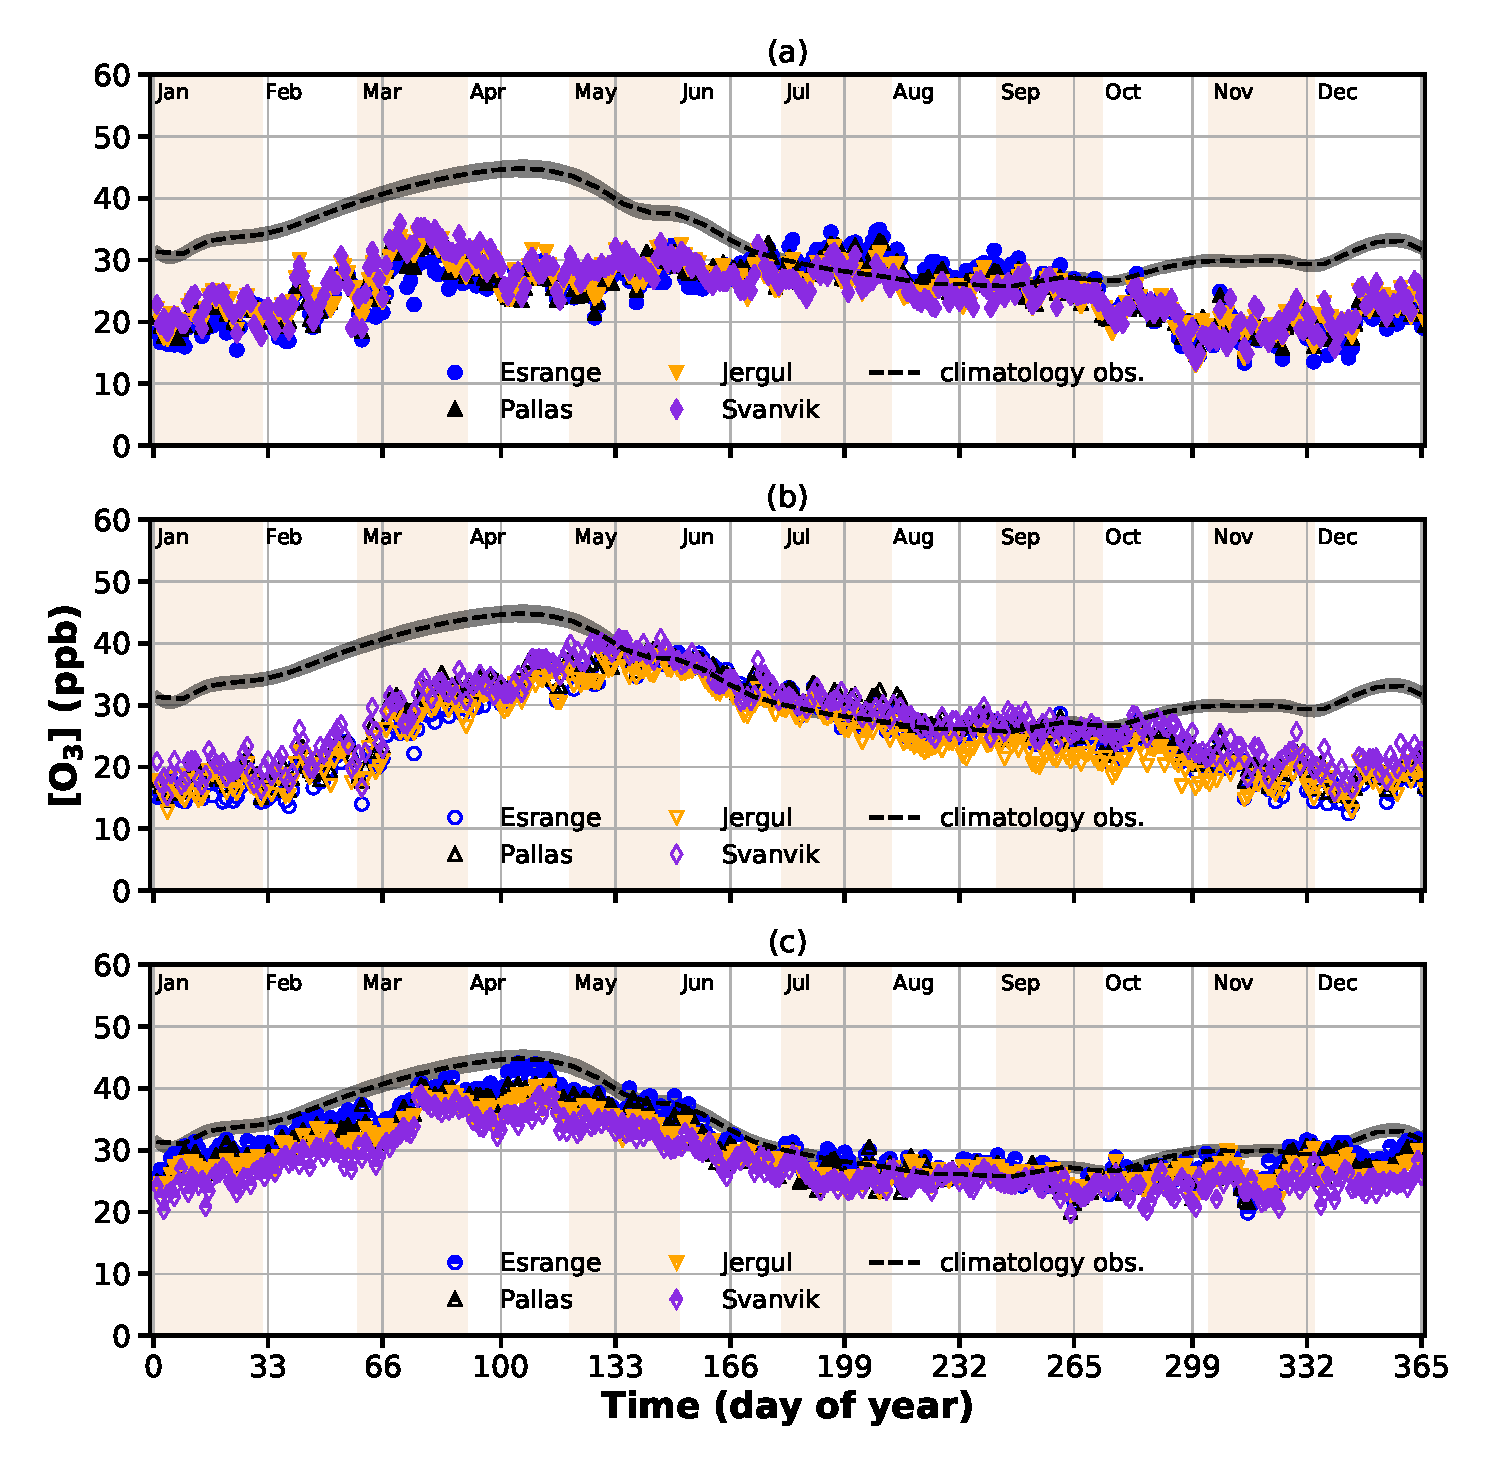
\includegraphics[width=8.3cm]{ozone_climatologies_portrait}
  \caption{Comparison of climatologies derived from observational data (EBAS, see Fig.~\ref{fig:ozone_climatology_fenoscandic_obs}) with various ozone reanalysis products: (a) ECMWF: MACC reanalysis; (b) ECMWF: CAMS reanalysis; (c) Copernicus: Regional model reanalysis ensemble mean. As representative for the sites, the nearest neighboring grid point has been chosen. The ECMWF products do not reproduce observed surface ozone well. The MACC reanalysis is in general too low and displays an erroneous seasonal cycle. The CAMS reanalysis matches better but does not reproduce the seasonality in northern Fennoscandia. The ensemble mean of the Copernicus regional model reanalysis does reproduce the seasonal cycle in northern Fennoscandia, though the modeled ozone concentrations are slightly too low.}
  \label{fig:ozone_climatologies}
\end{figure}

There are many probable explanations for the discovered differences in the climatologies derived from the three reanalyses. The effective changes from the MACC reanalysis to CAMSRA have been reported and discussed by \citet{ACP:Inness2019} on a global level. Amongst others, an assimilation of ozone profiles from satellite retrieval and an upgraded ozone chemistry scheme have lead to the enhanced performance of latter. The higher spatial resolution of the regional air quality models used in the CAMS Regional Ensemble compared to the global reanalyses does capture more localized depletion and peak episodes in \chem{[O_3]} better and enhances the capability of the models with respect to daily and seasonal cycles in ozone. Latter is, of course, also affected by upgrades in the OpenIFS used as meteorological forcing. However, we can assume that the main driver for the strikingly different results are the assimilated observational ozone data. Satellite retrievals resolve \chem{[O_3]} at the surface rather poorly and hence do not constrain the global models well enough \citet{ACP:Andersson2017}.

\subsection{2018/19 anomalies}
\label{subsec:anomalies}
Using these established climatologies, we look at the anomalies in 2018/19 and discuss the differences between the two years. 

\subsubsection{Temperature, precipitation, and global irradiance}
\label{subsubsec:anomal_tpq}
In Fig.~\ref{fig:plot_temperature_anomalies_svanvik}, temperature anomalies at Svanvik are shown as percentage of days warmer/colder than $\pm 1\,\sigma$ from the climatological mean for each month. Negative deviations from climatology are displayed as negative percentage. The full annual positive/negative deviations are indicated in the respective corners (right upper/right lower). The hatched area between the dashed lines indicates the expected percentage of values falling above/below $\pm 1\,\sigma$ if a normal distribution is assumed ($15.9\,\unit{\%}$). The summer of 2018 was significantly warmer than average. Especially in May and July more than $40\,\unit{\%}$ of days were significantly warmer than normal temperature. Temperatures continued to be significantly warmer throughout fall into early winter (August--November) with the exception of October. March 2018 was unusually cold. The summer of 2019 was fairly average, however significantly colder in July, while August was both significantly colder and warmer. Temperatures in April were significantly warmer than average.

\begin{figure}[t]
  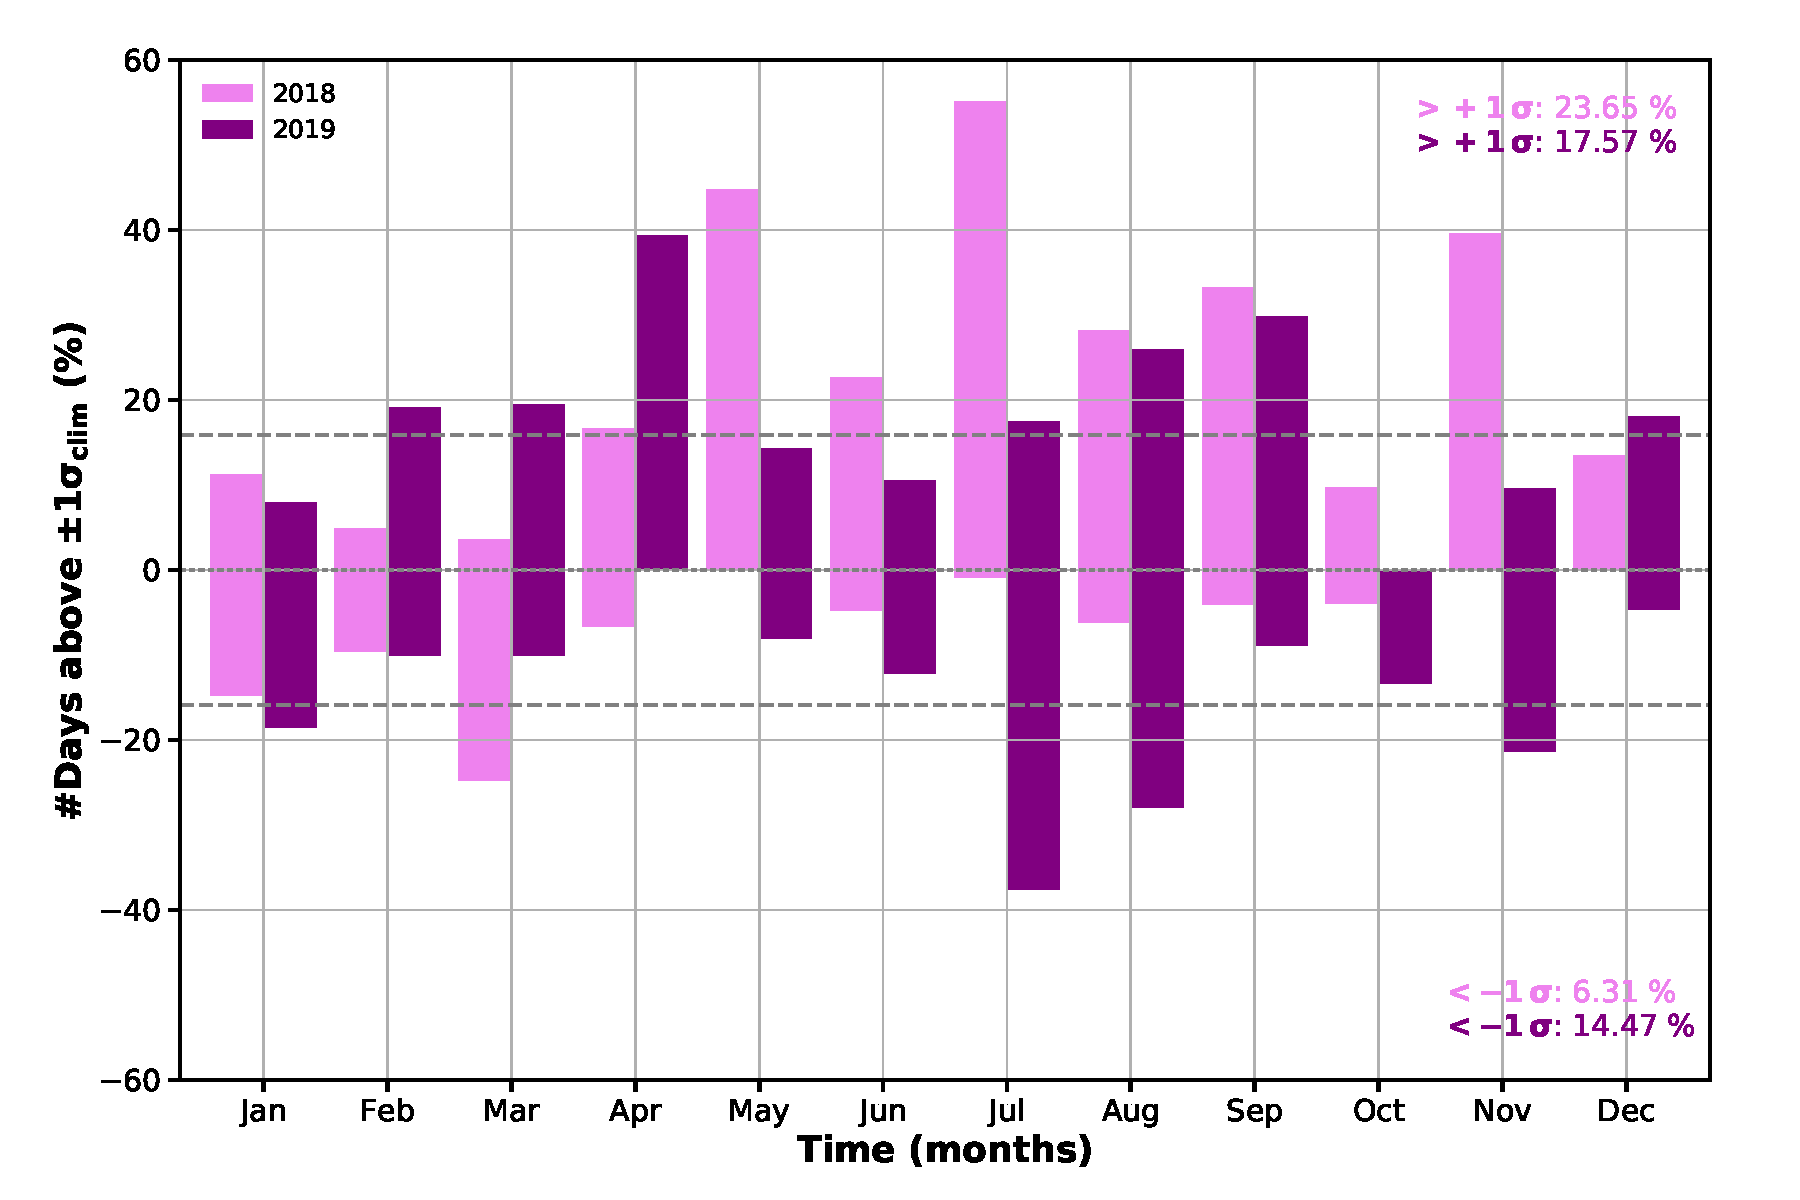
\includegraphics[width=8.3cm]{temperature_signific_1}
  \caption{Temperature anomalies at Svanvik. Percentage of days warmer/colder than $\pm 1\,\sigma$ from climatological mean displayed for each month. Negative deviations from climatology are shown as negative percentage. The annual positive/negative deviations are indicated in the respective corners (right upper/right lower). The hatched area between the dashed lines indicates the expected percentage of values falling above/below $\pm 1\,\sigma$ if a normal distribution is assumed ($15.9\,\unit{\%}$). The summer of 2018 was significantly warmer than average, especially May and July. The summer of 2019 was fairly average but significantly warmer than average in April and colder in July/August.}
  \label{fig:plot_temperature_anomalies_svanvik}
\end{figure}

In a similar way, the precipitation anomalies at Svanvik are displayed in Fig.~\ref{fig:plot_precipitation_anomalies_svanvik}. However, the percentage of days wetter/drier than $\pm \frac{1}{2}\,\sigma$ from the climatological mean is shown for each month, due to the larger variability in observed precipitation too few days showed a significance of $1 \sigma$ or higher. As above, negative deviations from the climatology are shown as negative percentage and annual positive/negative deviations are indicated in the respective corners. The hatched area between the dashed lines indicates the expected percentage of values falling above $\pm\frac{1}{2}\,\sigma$ if a normal distribution is assumed ($30.8\,\unit{\%}$). Unlike for the temperature anomalies, the picture is not as clear. While March 2018 was unusually wet, summer and fall (May/July, September/October) were significantly drier than average. 2019 was rather average throughout the year, with drier than usual fall (September/October) and a wet December.

\begin{figure}[t]
  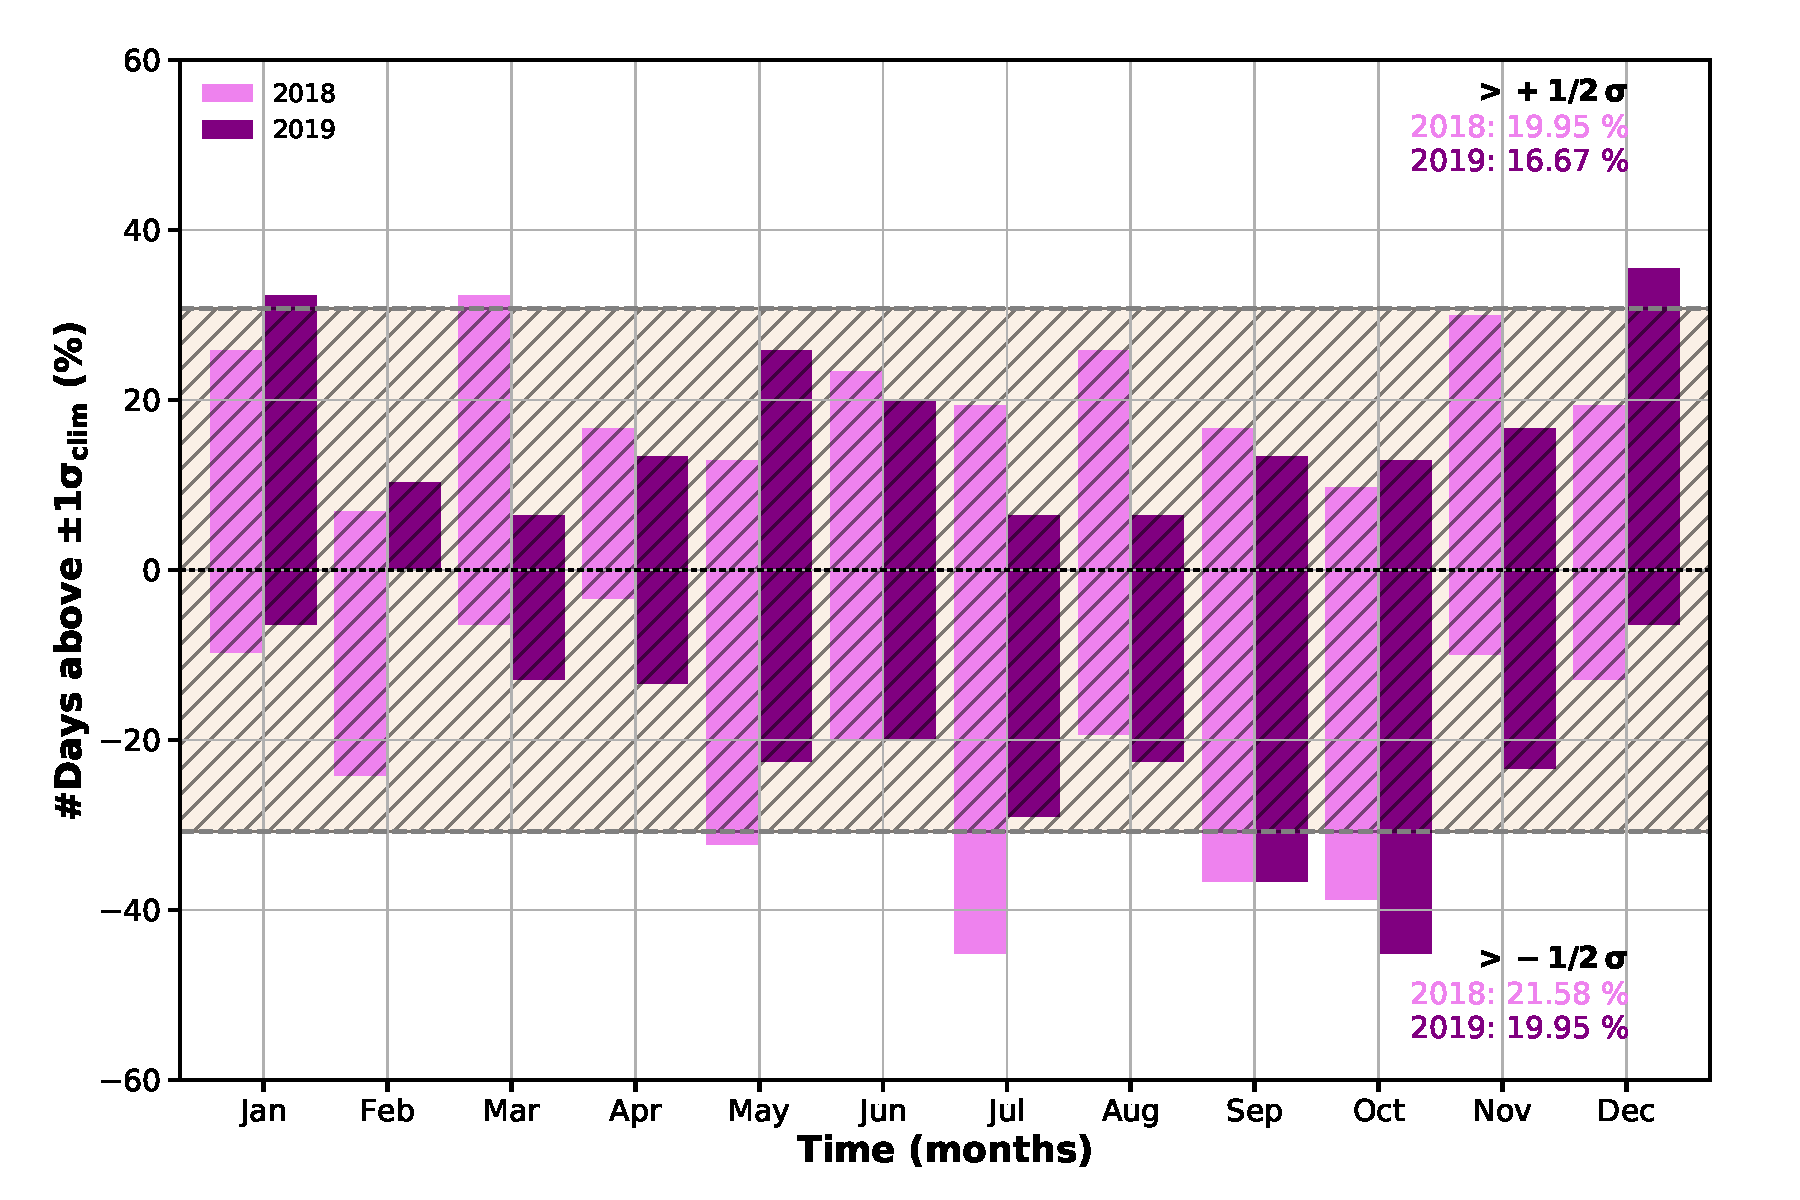
\includegraphics[width=8.3cm]{precipitation_signific_1}
  \caption{Precipitation anomalies at Svanvik. Percentage of days wetter/drier than $\pm \frac{1}{2}\,\sigma$ from climatological mean displayed for each month. Negative deviations from climatology are shown as negative percentage. The annual positive/negative deviations are indicated in the respective corners (right upper/right lower). The hatched area between the dashed lines indicates the expected percentage of values falling above $\pm\frac{1}{2}\,\sigma$ if a normal distribution is assumed ($30.8\,\unit{\%}$). Summer was significantly dry only in 2018, while fall was significantly dry in both years.}
  \label{fig:plot_precipitation_anomalies_svanvik}
\end{figure}

Similarly, the global irradiance anomalies at Svanvik are presented in Fig.~\ref{fig:global_rad_signific}. The percentage of days above/below $\pm 1\,\sigma$ from the climatological mean is displayed for each month. The hatched area between the dashed lines indicates the expected percentage of values falling above/below $\pm 1\,\sigma$ if a normal distribution is assumed. In summer 2018 (May/July), global irradiance was significantly higher than on average, while 2019 was generally an average year with a slightly darker spring (April/May).

\begin{figure}[t]
  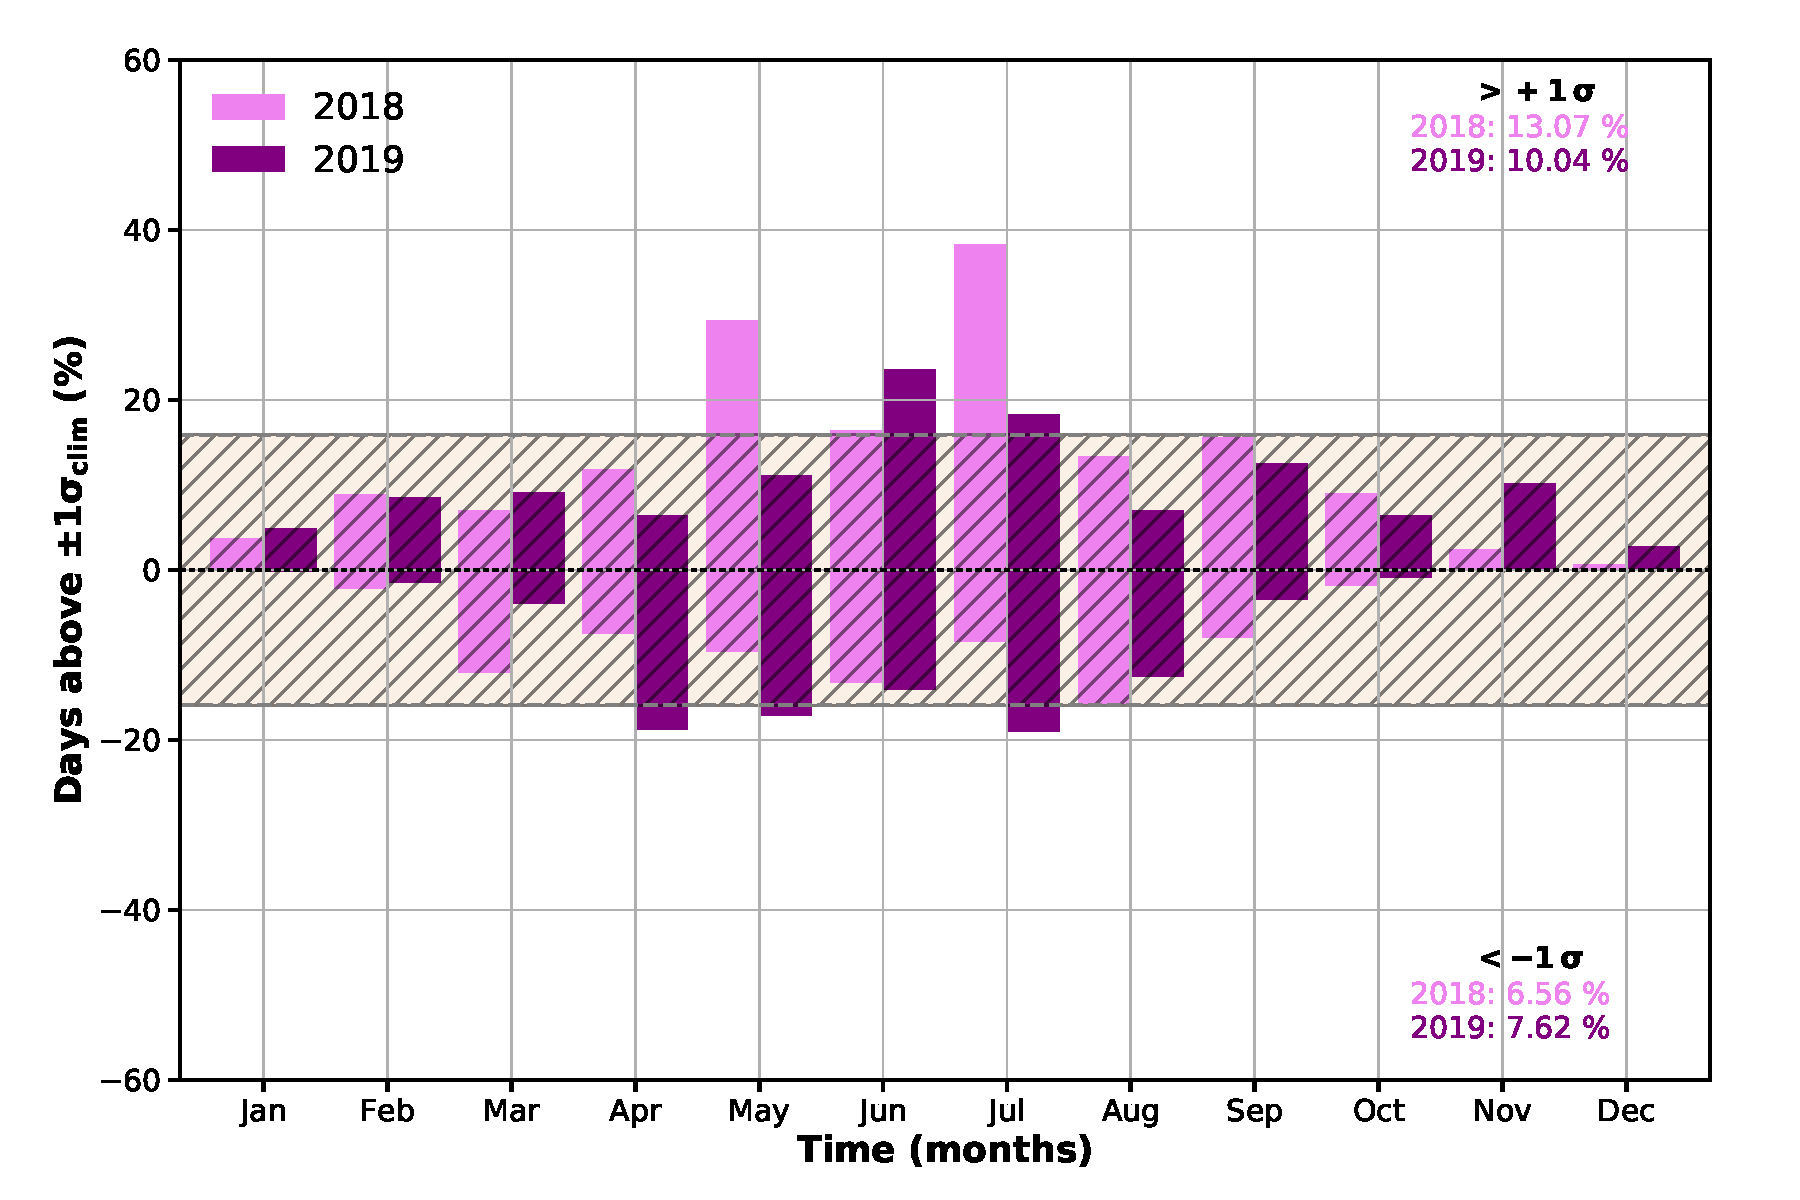
\includegraphics[width=8.3cm]{global_rad_signific_1}
  \caption{Global irradiance anomalies at Svanvik. Percentage of days above/below $\pm 1\,\sigma$ from climatological mean displayed for each month. Negative deviations from climatology are shown as negative percentage. The annual positive/negative deviations are indicated in the respective corners (right upper/right lower). The hatched area between the dashed lines indicates the expected percentage of values falling above/below $\pm 1\,\sigma$ if a normal distribution is assumed ($15.9\,\unit{\%}$). In summer 2018 (May/July), global irradiance was significantly higher than on average, while 2019 had significantly less than normal irradiance in April/May and more in June.}
  \label{fig:global_rad_signific}
\end{figure}

In summary, 2018 was significantly warmer, drier, and lighter than the climatological average, while 2019 was a rather average year.

\subsubsection{Ozone}
\label{subsubsec:anomal_ozone}
As we discussed in the preceding Section~\ref{subsubsec:anomal_tpq}, meteorological conditions in 2018 were significantly different from the climatological average. How does this translate into observed ozone anomalies \chem{\Delta[O_3]}?

If the data collected at Svanvik had been complete in 2018 and the climatology had extended into the resent past, we could have assessed the significance of ozone anomalies in the same way as for temperature, precipitation, and global irradiance. In Section~\ref{subsubsec:clim_ozone}, we described the construction of climatologies for northern Fennoscandia based on long term observations at Esrange, Jergul/Karasjok, and Pallas. For Svanvik this assessment is based on rather uncertain observations from 1986--1996. We also discussed the general patterns, similarities and differences. We shall now investigate \chem{\Delta[O_3]} in 2018/19 with respect to these climatologies in more detail.

In the following, we will use the interchangeable terms anomalies and residuals to distinguish between a climatological (anomalies) and a statistical (residuals) point of view.
All the above factors make it necessary to look not only at anomalies but statistically assess ozone concentration residuals at Svanvik as well as at Esrange and Pallas in comparison. Since the climatology of latter is more reliable, we will start with surface ozone concentration residuals \chem{\Delta[O_3]} at Esrange and Pallas in 2018. As data for 2019 has not yet been available from EBAS (last access, February 2020), we refrain from looking into these.

In Appendix Fig.~\ref{fig:ozone_climatology_fenoscandic_obs_residuals}, the probability density functions of daily mean ozone concentration residuals for Esrange and Pallas are shown. Both stations display a clear deviation from the climatological mean, however, not significant. On average, \chem{[O_3]} had been elevated by $(1.9\pm 5.7)\,\unit{ppb}$ and $(1.9\pm 5.4)\,\unit{ppb}$, respectively. Both distributions are slightly skewed towards positive deviations with $\frac{1}{4}$ of days (3. quantile, q3) falling above $5.8\,\unit{ppb}$ and $5.6\,\unit{ppb}$, respectively.

Appendix Figure~\ref{fig:ozone_climatology_fenoscandic_obs_residuals-Svanvik} displays the probability density functions of daily mean ozone concentration residuals for Svanvik based on data taken in 2018/19 with respect to the climatology derived for northern Fennoscandia (denoted NF in Appendix Fig.~\ref{fig:ozone_climatology_fenoscandic_obs_residuals-Svanvik}a) and the climatology derived for Svanvik (Appendix Fig.~\ref{fig:ozone_climatology_fenoscandic_obs_residuals-Svanvik}b).
As previously mentioned, \chem{\left<[O_3]\right>} at Svanvik are $(6.6\pm 7.1)\,\unit{ppb}$ lower than the northern Fennoscandic climatology. For 2018 and 2019, we find $\Delta\chem{\left<[O_3]\right>} = (-3.8\pm 5.6)\,\unit{ppb}$ and $\Delta\chem{\left<[O_3]\right>} = (-5.2\pm 5.0)\,\unit{ppb}$, respectively. While the probability density of the residuals between the two climatologies is skewed towards negative values, the skew of 2018/19 is positive.
With respect to the climatology for Svanvik (Appendix Fig.~\ref{fig:ozone_climatology_fenoscandic_obs_residuals-Svanvik}b), the probability density functions average for 2018/19 lies at $\Delta\chem{\left<[O_3]\right>} = (2.6\pm 5.8)\,\unit{ppb}$ and $\Delta\chem{\left<[O_3]\right>} = (1.2\pm 5.0)\,\unit{ppb}$, respectively.
Neither of the \chem{\Delta\left<[O_3]\right>} is significant by statistical means, but daily average ozone concentrations are slightly elevated in 2018 compared to 2019.

The \chem{\left<\Delta\left<[O_3]\right>\right>} for Svanvik in 2018 is slightly larger than for Esrange and Pallas. This could mean either that 2018 had been more exceptional at Svanvik or the derived climatology may need a correction for increased tropospheric background ozone concentration. Based on the meteorological conditions, we assume 2019 as average year which leads to a constant bias of about $1.2\,\unit{ppb}$. Daily \chem{\Delta_{present-past}\left<[O_3]\right>} from Esrange and Pallas, wherein present is defined as the average of 2010--2018 and past as the respective beginning of data taking until 1997, do not reveal a clear trend: We find for Esrange $(1.5\pm 3.1)\,\unit{ppb}$ and for Pallas $(-2.5\pm 3.7)\,\unit{ppb}$ \citep{NILU2003, BER:Ruoho-Airola2015}. Former is compatible with our assumed bias for the climatology derived for Svanvik.

To further investigate the ozone residuals, we conduct a Student's~t-test ($t = \frac{\chem{\Delta[O_3]}}{\sigma}$), assuming the same sample uncertainty $\sigma$ in both, climatology and the year in question. Results for Esrange and Pallas are shown in Appendix Fig.~\ref{fig:ozone_climatology_fenoscandic_obs_test}. This t-test clearly shows, that at both sites the residuals are significant on the $1\sigma$ level for at least $50\,\unit{\%}$. In Appendix Fig.~\ref{fig:ozone_climatology_fenoscandic_obs_test-Svanvik}, the test statistics for Svanvik are displayed. From Appendix Fig.~\ref{fig:ozone_climatology_fenoscandic_obs_test-Svanvik}a), we can deduce, that the residuals between the Svanvik climatology and the northern Fennoscandic climatology are significant on the $2\sigma$ level for at least half of the data, while the residuals are less certain in 2018 and 2019. In Appendix Fig.~\ref{fig:ozone_climatology_fenoscandic_obs_test-Svanvik}b) the same is shown for the years 2018/19 with respect to the climatology from Svanvik. We find that less than $50\,\unit{\%}$ of ozone concentration residuals are significant on the $1\sigma$ level.

In accordance to the above findings, we adjust the derived ozone climatology for Svanvik by adding a constant bias correction factor $\Delta\chem{[O_3]_\mathrm{bias-corr}} = 1.2\,\unit{ppb}$ and estimate the ozone concentration anomalies for 2018/19. In Fig.~\ref{fig:ozone_signific}, the resulting percentage of days above/below $\pm 1\,\sigma$ from the bias-corrected climatological mean is displayed for each month. Negative deviations from climatology are shown as negative percentage. Note that missing bars for certain months are both due to data availability (see Section~\ref{subsubsec:atmo_svanvik} for details about the time range of data taking at Svanhovd) and anomalies not meeting the criteria of $\pm 1\sigma$ deviation from climatological mean. In April/May 2018, ozone was significantly enhanced, while 2019 was generally an average year. In both years, ozone concentrations were significantly below average in November. July 2018 has not been corrected for the missing data due to data acquisition problems. The corrected value is, however, indicated by the star (refer to Section~\ref{subsec:ozone_reco} for details of the used method for gap filling).

\begin{figure}[t]
  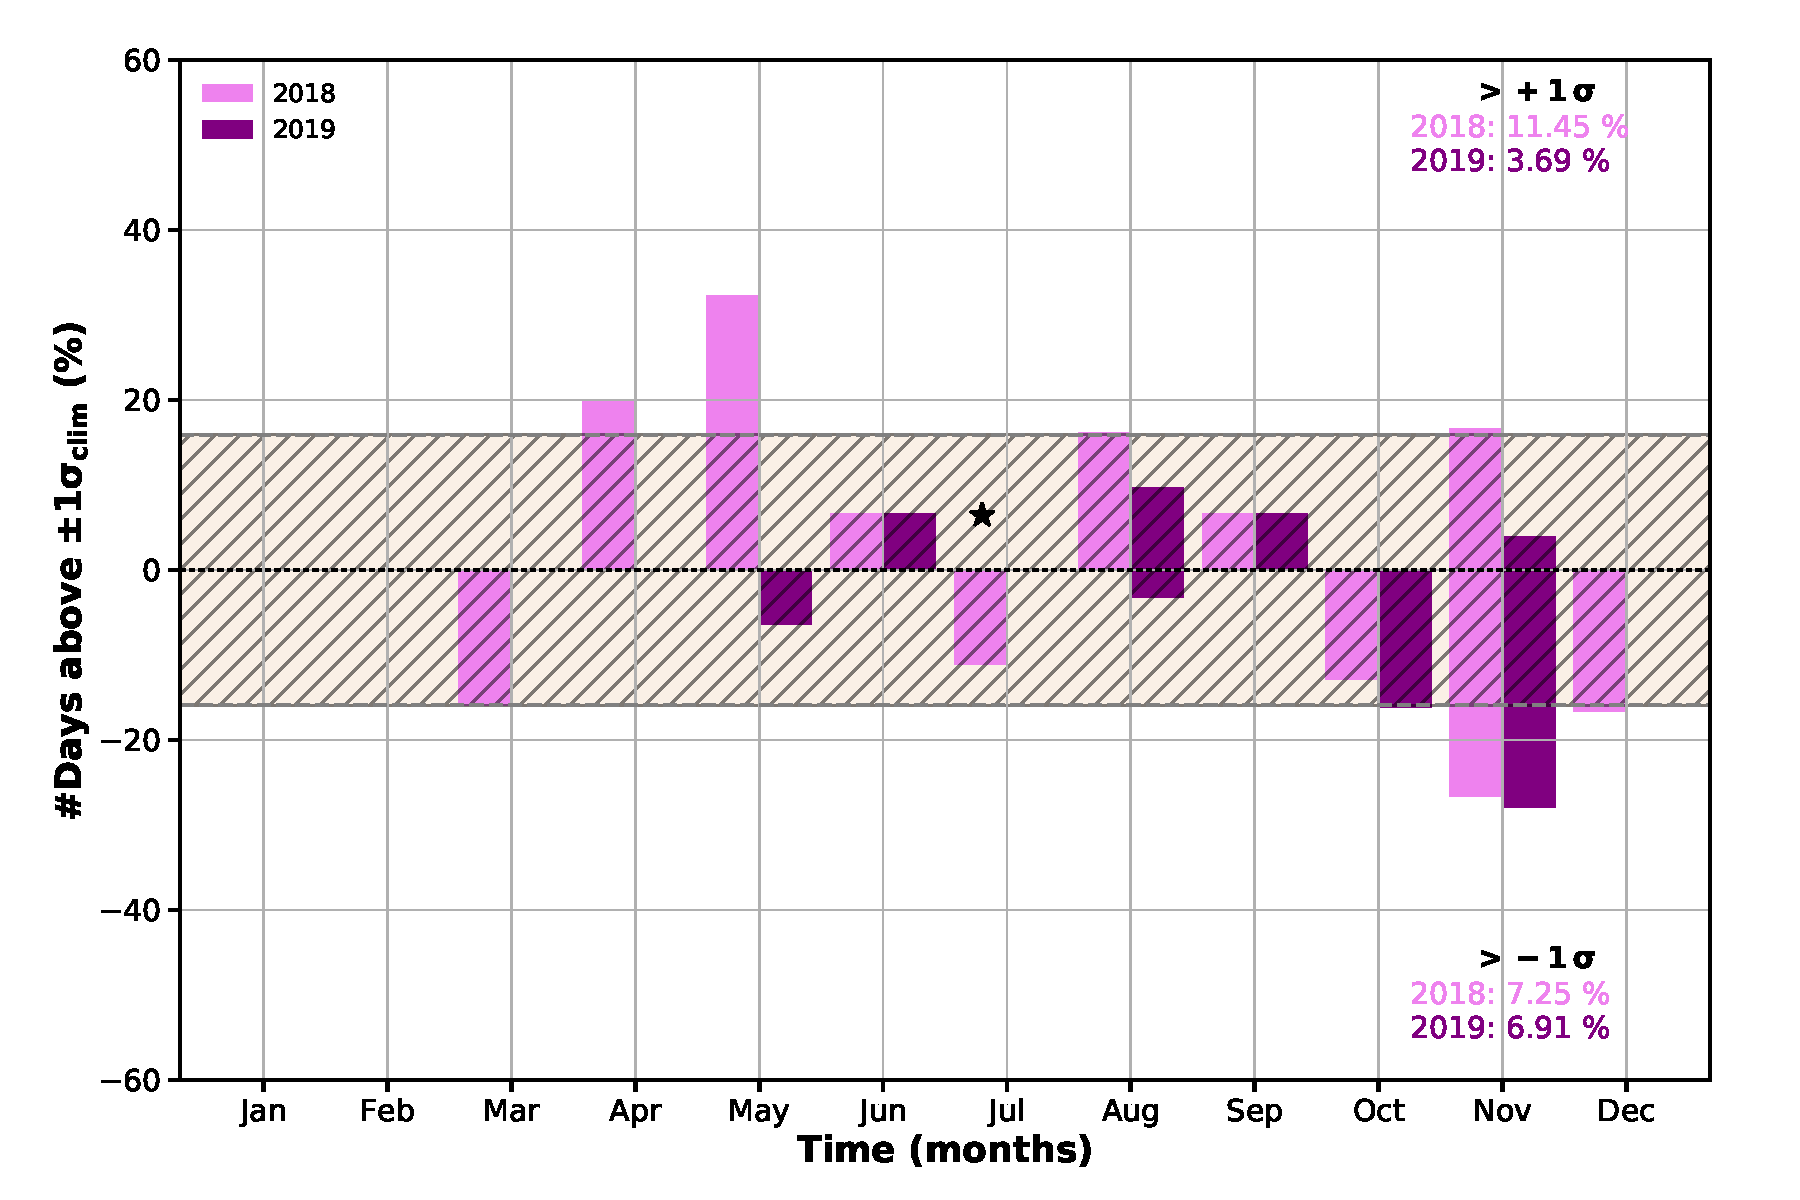
\includegraphics[width=8.3cm]{ozone_signific_1}
  \caption{Ozone concentration anomalies at Svanvik. Ozone climatology has been corrected for an constant negative bias of $-1.2\,\unit{ppb}$. Percentage of days above/below $\pm 1\,\sigma$ from climatological mean displayed for each month. Negative deviations from climatology are shown as negative percentage. The annual positive/negative deviations are indicated in the respective corners (right upper/right lower). The hatched area between the dashed lines indicates the expected percentage of values falling above/below $\pm 1\,\sigma$ if a normal distribution is assumed ($15.9\,\unit{\%}$). July 2018 has not been corrected for the missing data due to data acquisition problems. The corrected value is indicated by the star (refer to Section~\ref{subsec:ozone_reco} for details). In April/May 2018, ozone was significantly higher than on average, while 2019 was generally an average year. In both years ozone concentrations were significantly below average in November.}
  \label{fig:ozone_signific}
\end{figure}

To conclude, ozone concentrations in 2018 have been elevated compared to the respective climatologies, however, on average not significantly by statistical means. At Esrange and Pallas at least $25\,\unit{\%}$ (3.~quantile) of anomalies are significant on a $3\sigma$ level or more, while at Svanvik the 3.~quantile lies at about $2\sigma$. This means that in 2018 the stations at Esrange and Pallas saw more days with elevated ozone than was monitored at Svanvik.

\section{DO3SE modeling}
\label{sec:do3se}
To investigate which of the environmental factors lead to the observed ozone damage on clover and tobacco in 2018 in contrast to 2019, when no such damage was found on the clovers but only on the sensitive tobacco cultivar, we model the ozone uptake using the $\mathrm{DO_3SE}$ model and give an estimate on biomass reduction due to ozone uptake.

\subsection{Model description}
\label{subsec:model_describtion}

The opening of stomata is governed by different species-specific and environmental factors and can be described by a multiplicative model \citep{PTRS:Jarvis1976,ICP:MappingManual2017}:
\begin{equation}
  g^k_\text{sto} = g^k_\text{max} \cdot f^k_\text{phen} \cdot f^k_\text{light} \cdot \max{\left\{f^k_\text{min}, f^k_\mathrm{T} \cdot f^k_\mathrm{VPD} \cdot f^k_\text{SW}\right\}}.
  \label{eq:stomatal}
\end{equation}
%
Where $g_\mathrm{max}$ is the specific-specific maximum stomatal conductance value which is then modified by seasonal and environmental factors that vary within a range $0-1$. They are empirically determined and account for leaf phenology ($f_\text{phen}$), light ($f_\text{light}$), temperature ($f_\mathrm{T}$), water vapor pressure deficit ($f_\mathrm{VPD}$), and soil water content ($f_\text{SW}$). All factors differ with species or plant functional type (PFT) denoted with $k$.

The temperature adjustment function is defined as
%
\begin{equation}
  f_\mathrm{T} = \frac{T_\text{air}-T_\text{min}}{T_\text{opt}-T_\text{min}} \cdot \left(\frac{T_{\text{max}}-T_\text{air}}{T_{\text{max}}-T_\text{opt}}\right)^\beta,
  \label{eq:f_temp}
\end{equation}
with $\beta = \frac{T_\text{max}-T_\text{opt}}{T_\text{opt}-T_\text{min}}$ a mixed reciprocal polynomial function of temperature. The shape parameters $T_\text{min}$, $T_\text{max}$ and $T_\text{opt}$ are tabulated for various species or PFT and $T_\mathrm{air}$ is the surface air temperature. All temperatures are defined in units of \unit{^\circ C}.

The water vapor pressure deficit function is
%
\begin{equation}
  f_\mathrm{VPD} = f_\text{min}+(1-f_\text{min}) \cdot \frac{D_\text{min} - \text{VPD}}{D_\text{min}-D_\text{max}}
  \label{eq:f_vpd}
\end{equation}
%
where VPD is the leaf to air vapor pressure deficit in \unit{kPa} with $f_\text{min}$, $D_\text{min}$, $D_\text{max}$ describing the relative stomatal conductance to changes in vapor pressure deficit.

The wavelength band $400-700\,\unit{nm}$ plant chlorophyll responds to is called photosynthetic active radiation (PAR). Its integral is the photosynthetic photon flux density (PPFD). The relationship between relative $g_\mathrm{sto}$ and PPFD is given by
%
\begin{equation}
  f_\text{light} = 1-\text{exp}(-\alpha_\text{light}\cdot \text{PPFD})
  \label{eq:flight}
\end{equation}
%
where $\alpha_\mathrm{light}$ is a slope parameter describing how fast stomata open or close at low light intensities.

The $\mathrm{DO_3SE}$ model as described in \citet{ACP:Bueker2012} is used to simulate SWP across a species or PFT specific root depth according to the Penman--Monteith energy balance method that drives water cycling through the soil--plant--atmosphere system. \citet{ACP:Bueker2012} discuss several formulations available to parameterize the reduction in stomata conductance due to water content in the soil. Here we use the relationship between reative $g_\mathrm{sto}$ and soil water potential (SWP) given by:
%
\begin{equation}
  f_\mathrm{SW} = \text{min}\left\{1, \text{max}\left\{f_\mathrm{min}, \frac{(1 - f_\mathrm{min})\cdot(\mathrm{SWP_{min}} - \mathrm{SWP})}{\mathrm{SWP_{min}} - \mathrm{SWP_{max}}} + f_\mathrm{min} \right\} \right\}
    \label{eq:fsw}
\end{equation}
%
where SWP is the soil water potential across the root zone and $\mathrm{SWP_{min}}$ and $\mathrm{SWP_{max}}$ are the paramters describing the $f_\mathrm{SW}$ relationship.

To compute $\mathrm{POD_y}$, we estimate the stomatal \chem{O_3} flux ($\Phi_\mathrm{sto}$) based on the assumption that the concentration of \chem{O_3} at the top of the canopy represents a reasonable estimate of the concentration at the upper surface of the laminar layer for a sunlit upper canopy leaf. The terms $r_c$ (leaf surface resistance) and $r_b$ (quasi-laminar resistance) allow for the deposition of \chem{O_3} to the leaf and the fraction that is taken up via the stomata. 
%
\begin{equation}
  \Phi_\mathrm{sto} = \chem{[O_3]} \cdot \frac{u(z_1) \cdot g_\mathrm{sto} \cdot r_c}{r_b + r_c}.
  \label{eq:flux_stomata}
\end{equation}
%
The quasi-laminar boundary layer resistance is calculated by
%
\begin{equation}
  r_b = 1.3 \cdot 150 \cdot \sqrt{\frac{L}{u(z_1)}}.
  \label{eq:quasi_laminar_resist}
\end{equation}
%
Where $L$ is the cross-wind leaf dimension, $u(z_1)$ the wind speed at height $z_1$, and the factor $1.3$ accounts for the diffusivities between heat and \chem{O_3}. 

\subsection{Input data and gap filling methodology}
\label{subsec:ozone_reco}
The $\mathrm{DO_3SE}$ model requires hourly, continuous meteorological observations. In addition to variables covered in Section~\ref{sec:data}, $2\,\unit{m}$ wind $u_\text{2m}$ and vapor pressure deficit VPD are needed. VPD has been calculated from observed $T_\text{2m}$ and relative humidity
\begin{equation}
  \text{VPD} = P_s(T) \cdot \left(1-\frac{\text{relHum}}{100}\right),
\end{equation}
with saturation vapor pressure $P_s(T)$ in \unit{hPa} derived from Arden Buck equation~\citep{JAP:Buck1981, Buck2012}.
  
The following gap filling methodology was devised for the meteorological input data:
\begin{itemize}
\item Single hours of missing data were filled by taking the average of the hourly values coming before, and after, the missing value.
\item Several consecutive hours of missing data (23 or less) were filled by taking the average of the corresponding hour the day before, and the day after; and repeating this for each missing hour of data. If data was unavailable from that hour of the previous day, then only the value from the day after was used and vice versa. Interpolated values were not used in calculating averages.
\item Data gaps longer than $24\,\unit{h}$ were filled using weekly diurnal averages. i.e. an average was calculated using the corresponding hour throughout the week before and after. Interpolated values were not used in calculating averages.
\end{itemize}

Because the available reanalysis products for surface ozone have their limitations, we deem it necessary to reconstruct the missing data in 2018 for the purpose of $\mathrm{DO_3SE}$ modeling by applying a Reynolds's decomposition of the form:
\begin{equation}
  \chem{[O_3]} = \chem{\left<[O_3]\right>} + \chem{\Delta[O_3]},
  \label{eq:reynolds_decomp}
\end{equation}
with climatology \chem{\left<[O_3]\right>} and anomalies \chem{\Delta[O_3]}.
The exact procedure will be described in the following.
We derive hourly climatologies for individual stations and combine Esrange/Pallas to derive a climatology for northern Fennoscandia for July (Appendix Fig.~\ref{fig:ozone_reconstruction_2018_07}a). We compute temporal correlations between Svanvik and the other stations in northern Fennoscandia to estimate a time lag (Appendix Fig.~\ref{fig:time_lag_correlation}. We find $3\,\unit{h}$ for Esrange and Pallas with respect to Svanvik. Due to the high correlation with Svanvik (Appendix~Fig.~\ref{fig:density_distribution}), we decide on Pallas as reference station for the reconstruction. We correct the Fennoscandic climatology for the found time lag \chem{\left<[O_3]\right>_{hourly,\,t-3}} by shifting the respective time series back in time by $3\,\unit{h}$ and use it to derive a projection for Svanvik:
\begin{equation}
  X = \frac{\chem{\left<[O_3]\right>_{hourly}^{Svanvik}}}{\chem{\left<[O_3]\right>_{hourly,\,t-3}}}.
  \label{eq:mapping}
\end{equation}
As an intermediate step, we apply Eq.~(\ref{eq:reynolds_decomp}) to derive hourly anomalies for each station $i$
\begin{equation}
  \chem{\Delta[O_3]_{hourly}}^i = \chem{[O_3]_{hourly}}^i-\chem{\left<[O_3]\right>_{hourly}},
\end{equation}
with $i \in \{\text{Esrange, Pallas, Svanvik\}}$.
In Appendix Fig.~\ref{fig:ozone_reconstruction_2018_07}b), these hourly ozone concentration anomalies are shown. We also correct the ozone anomalies for Pallas for the time lag \chem{\Delta[O_3]_{hourly,\,t-3}^{Pallas}} and use the mapping function in Eq.~(\ref{eq:mapping}) to derive reconstructed anomalies for the missing values at Svanvik:
\begin{equation}
    \chem{\Delta [O_3]_{hourly}^{Svanvik,\,reco}} = \chem{\Delta[O_3]_{hourly,\,t-3}^{Pallas}} \cdot X
\end{equation}
Finally, we add the bias corrected Svanvik ozone climatology and derive a reconstructed ozone concentration time series \chem{[O_3]_{hourly}^{Svanvik,\,reco}}. In Appendix Fig.~\ref{fig:ozone_reconstruction_2018_07}c), the result is shown together with the observed data and the Copernicus Regional Model Reanalysis at the nearest grid point for comparison.

\subsection{Model parameters}
We roughly estimated land use types for an approximately $1\times 1\,\unit{km}$ patch centered at the NIBIO Environment Centre Svanhovd from Fig.~\ref{fig:svanhovd_research_station}: $48\,\unit{\%}$ grassland, $32.5\,\unit{\%}$ deciduous, $12.5\,\unit{\%}$ coniferous, $2\,\unit{\%}$ urban.

Default PFTs are derived from \citet{ICP:MappingManual2017} and will be referred to as \emph{mapping manual} abbrieved MM. A comprehensive list of these model parameters can be found in Supplement~Table~S1.
Intitial test simulations with the mapping manual derived PFTs showed unrealistically low $g_\mathrm{sto}$ in 2019 (Supplememt~Figs.SX--SX+2) particularly for grassland. Only during an extended periode in late July did we find substential stomatal conductance. In ecological terms, this would mean that there was almost no growth of grass in the summer of 2019 -- a prediction which is easily falsified by reality. We identified $f_\mathrm{T}$ as abnormally low, being the limiting factor of stomatal conductance. We propose bespoke parameterizations for the main vegetation types Norway spruce, birch, and perennial grassland better adapted to the climatic conditions in the target region.
Note that these parameterizations represent hypothetical PFTs or species that have to be varified by experiements. 

We hypothize that perannial vegetation will likely prioritize their growth or fast adolesence throughout the short, sub-boreal growing season and hence their carbon sequestration. Since the $\mathrm{DO_3SE}$ in its current state does not simulate $A_\mathrm{n}$, we assume for out purpose a first order proptionality between carbon uptake (photosynthesis) and $g_\mathrm{sto}$ and tune the species temperature and light response functions ($f_\mathrm{T}$ and $f_\mathrm{light}$) seperately for higher stomatal conductance. For this purpose, we graphically intersected propability density functions (PDFs) of climatological data for temperature and global irradiace with the respective response function (Fig.~\ref{fig:f_temp_grassland} for grassland; for Norway spruce and birch see Appendix Figs.~\ref{fig:f_temp_spruce}--\ref{fig:f_temp_birch}). Formally, a parameterization is considered more optimial the larger the intersection area between the response function and PDF is. 

For the climatization of the temperature response functions, we assume two different types: \emph{boreal} and \emph{cold}. In either cases, we further assume that the hypothetical species are more tolerant to cold conditions than the mapping manual default suggests and shift $f_\mathrm{T}$ towards colder temperatures. We construct \emph{cold} as representative for a species that is more tolerant to cold temperatures, but slightly less efficient at warm temperatures compared to the mapping manual default. In the same way, \emph{boreal} refers to a hypothetical species which is very tolerant to cold but is sensitive to high temperatures, and most efficient at cool temperatures (close to the climatological mean temperature of 1992--2000). All three types for grassland are depicted together with the temperature PDF in Fig.~\ref{fig:f_temp_grassland}a).

For Norway spruce, our hypothetical PFTs $T_\mathrm{opt}$ are motivated by a longer timeseries of both observed \chem{CO_2} uptake and temperature at two observation sites in Southern (\emph{cold}) and Northern (\emph{boreal}) Finland presented in \citet{TB:Kolari2007}. We assume a similar adaption in birch. The parameters are comprehensibly listed in Table~\ref{tab:sensitivity_tests_temp}.

For the the senisitivity regarding light, we assume that the plants may react either faster or slower to a change at lower light intensities. We analytically derive the inverse function $f_{\mathrm{light},k}^{-1}$ for each PFT or species $k$
\begin{equation}
  \gamma_k(f_\mathrm{light}) := f_{\mathrm{light}, k}^{-1} = -\frac{\ln(1-f_\mathrm{light})}{\alpha_k}.
  \label{eq:inverse_function}
\end{equation}
We calculate it for the mapping manual $\alpha_\mathrm{MM}$ at its halfway value $0.5$ 
\begin{equation}
  \gamma(0.5) = -\frac{\ln(0.5)}{\alpha_\mathrm{MM}},
  \label{eq:inverse_function_halfway}
\end{equation}
and define a variation $\gamma' = \gamma \cdot \epsilon$ with $\epsilon \in \{0.8, 1.2\}$. We resolve Eq.~(\ref{eq:inverse_function}) for $\alpha$ and derive $\alpha'(\gamma')$. The resulting functions are shown in Fig.~\ref{fig:f_temp_grassland}b). All derived parameters are given in Table~\ref{tab:sensitivity_tests_light}.

\begin{figure}[t]
  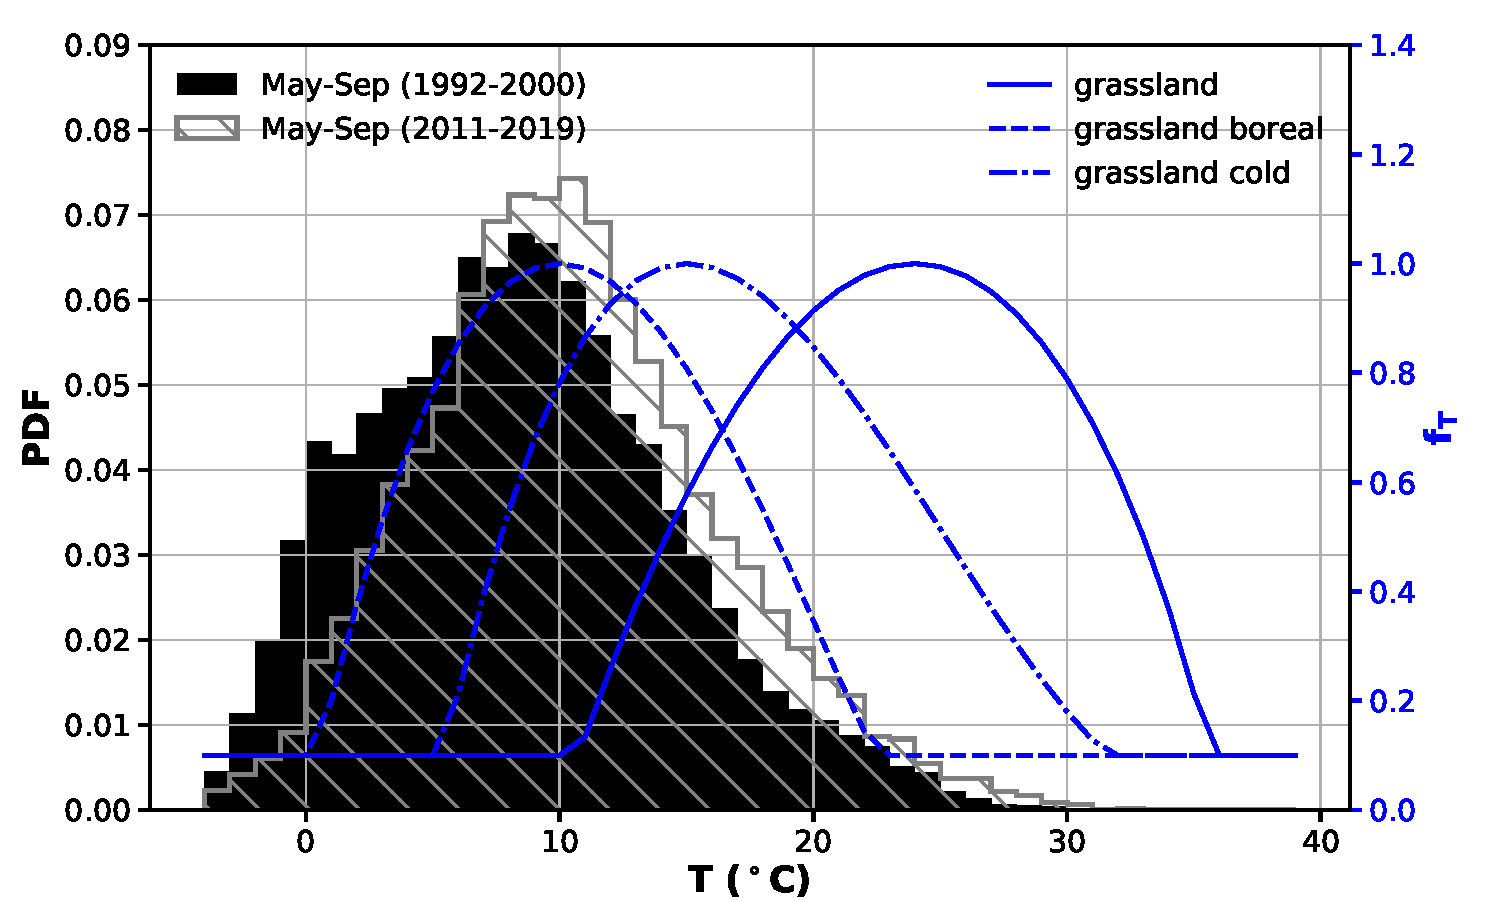
\includegraphics[width=8.3cm]{javis_funcs_temp_hist_grassland}\\
  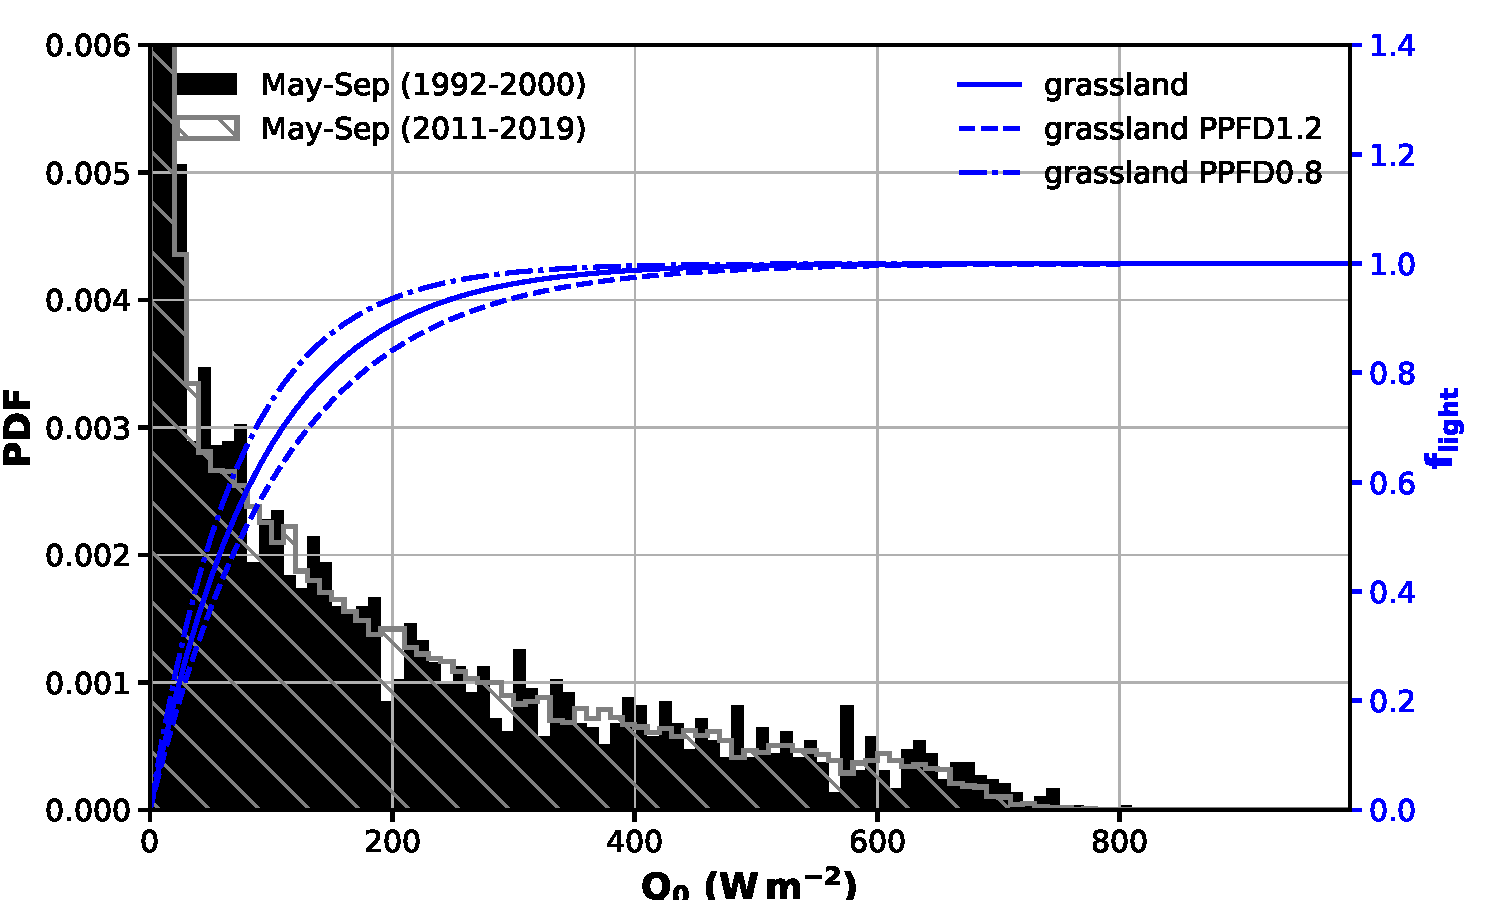
\includegraphics[width=8.3cm]{javis_funcs_rad_hist_grassland}
\caption{Construction of bespoke response functions for grassland. (a) $f_\mathrm{T}$ and (b) $f_\mathrm{flight}$ are shown toghether with underlying $T_\mathrm{air}$ and $Q_0$ climatologies (probability densitiy function - PDF), respectively. Original mapping manual parameterization is shown in comparison as solid line. Note that $Q_0$ has been truncated to $0.006$. PPFD0.8 and PPFD1.2 refer to $\alpha$ values increasing/decreasing PPFD at $f_\mathrm{light}=0.5$ by $\pm 20\,\%$, respectively.}
\label{fig:f_temp_grassland}
\end{figure}

\begin{table}[t]
  \caption{Bespoke temperature prameterizations. MM refers to mapping manual \citep{GCB:Mills2010,ICP:MappingManual2017}.}
  \label{tab:sensitivity_tests_temp}
  \begin{tabular}{llrrr}
    \tophline
    Species & type & $T_\mathrm{min}$ & $T_\mathrm{opt}$ & $T_\mathrm{max}$ \\
    \middlehline
    \multirow{3}{*}{Spruce} & MM & 0 & 20 & \multirow{3}{*}{100}\\
    & Boreal & 0 & 10 & \\
    & Cold & 0 & 15 & \\
    \middlehline
    \multirow{3}{*}{Birch} & MM & 5 & 20 & \multirow{3}{*}{100}\\
    & Boreal & 0 & 10\\
    & Cold & 5 & 15\\
    \middlehline
    \multirow{3}{*}{Grassland} & MM & 10 & 24 & 36\\
    & Boreal & 0 & 10 & 24 \\
    & Cold & 5 & 15 & 36\\
    \bottomhline
    \end{tabular}
\end{table}

\begin{table}[t]
  \caption{Bespoke light prameterizations. MM refers to mapping manual \citep{GCB:Mills2010,ICP:MappingManual2017}.}
  \label{tab:sensitivity_tests_light}
  \begin{tabular}{llr}
    \tophline
    Species & type & $\alpha$\\
    \middlehline
    \multirow{3}{*}{Spruce} & MM & 0.006 \\
    & PPFD0.8 & 0.008  \\
    & PPFD1.2 & 0.005  \\
    \middlehline
    \multirow{3}{*}{Birch} & MM & 0.004 \\
    & PPFD0.8 & 0.005\\
    & PPFD1.2 & 0.004\\
    \middlehline
    \multirow{3}{*}{Grassland} & MM & 0.011\\
    & PPFD0.8 & 0.014 \\
    & PPFD1.2 & 0.009 \\
    \bottomhline
    \end{tabular}
\end{table}


{\bf TODO: Write about boreal and cold parameter sets and their justification. Write about suggested method for optimizing PFTs in a simple but physiological way based on optimizing maximum climatological mean $g_\mathrm{sto}$ and morning responds. If plants have a short growing season up north optimizing \chem{CO_2} uptake around noon (highest light intensity) and speed up opening of stomata at lower intensities (morning), additional contraint lower climatological variance?}
An idea to justify our choice based on the fullset of climatological data for Svanvik is shown in Fig.~\ref{fig:javis_func_opt_mean}.

\begin{figure}[t]
  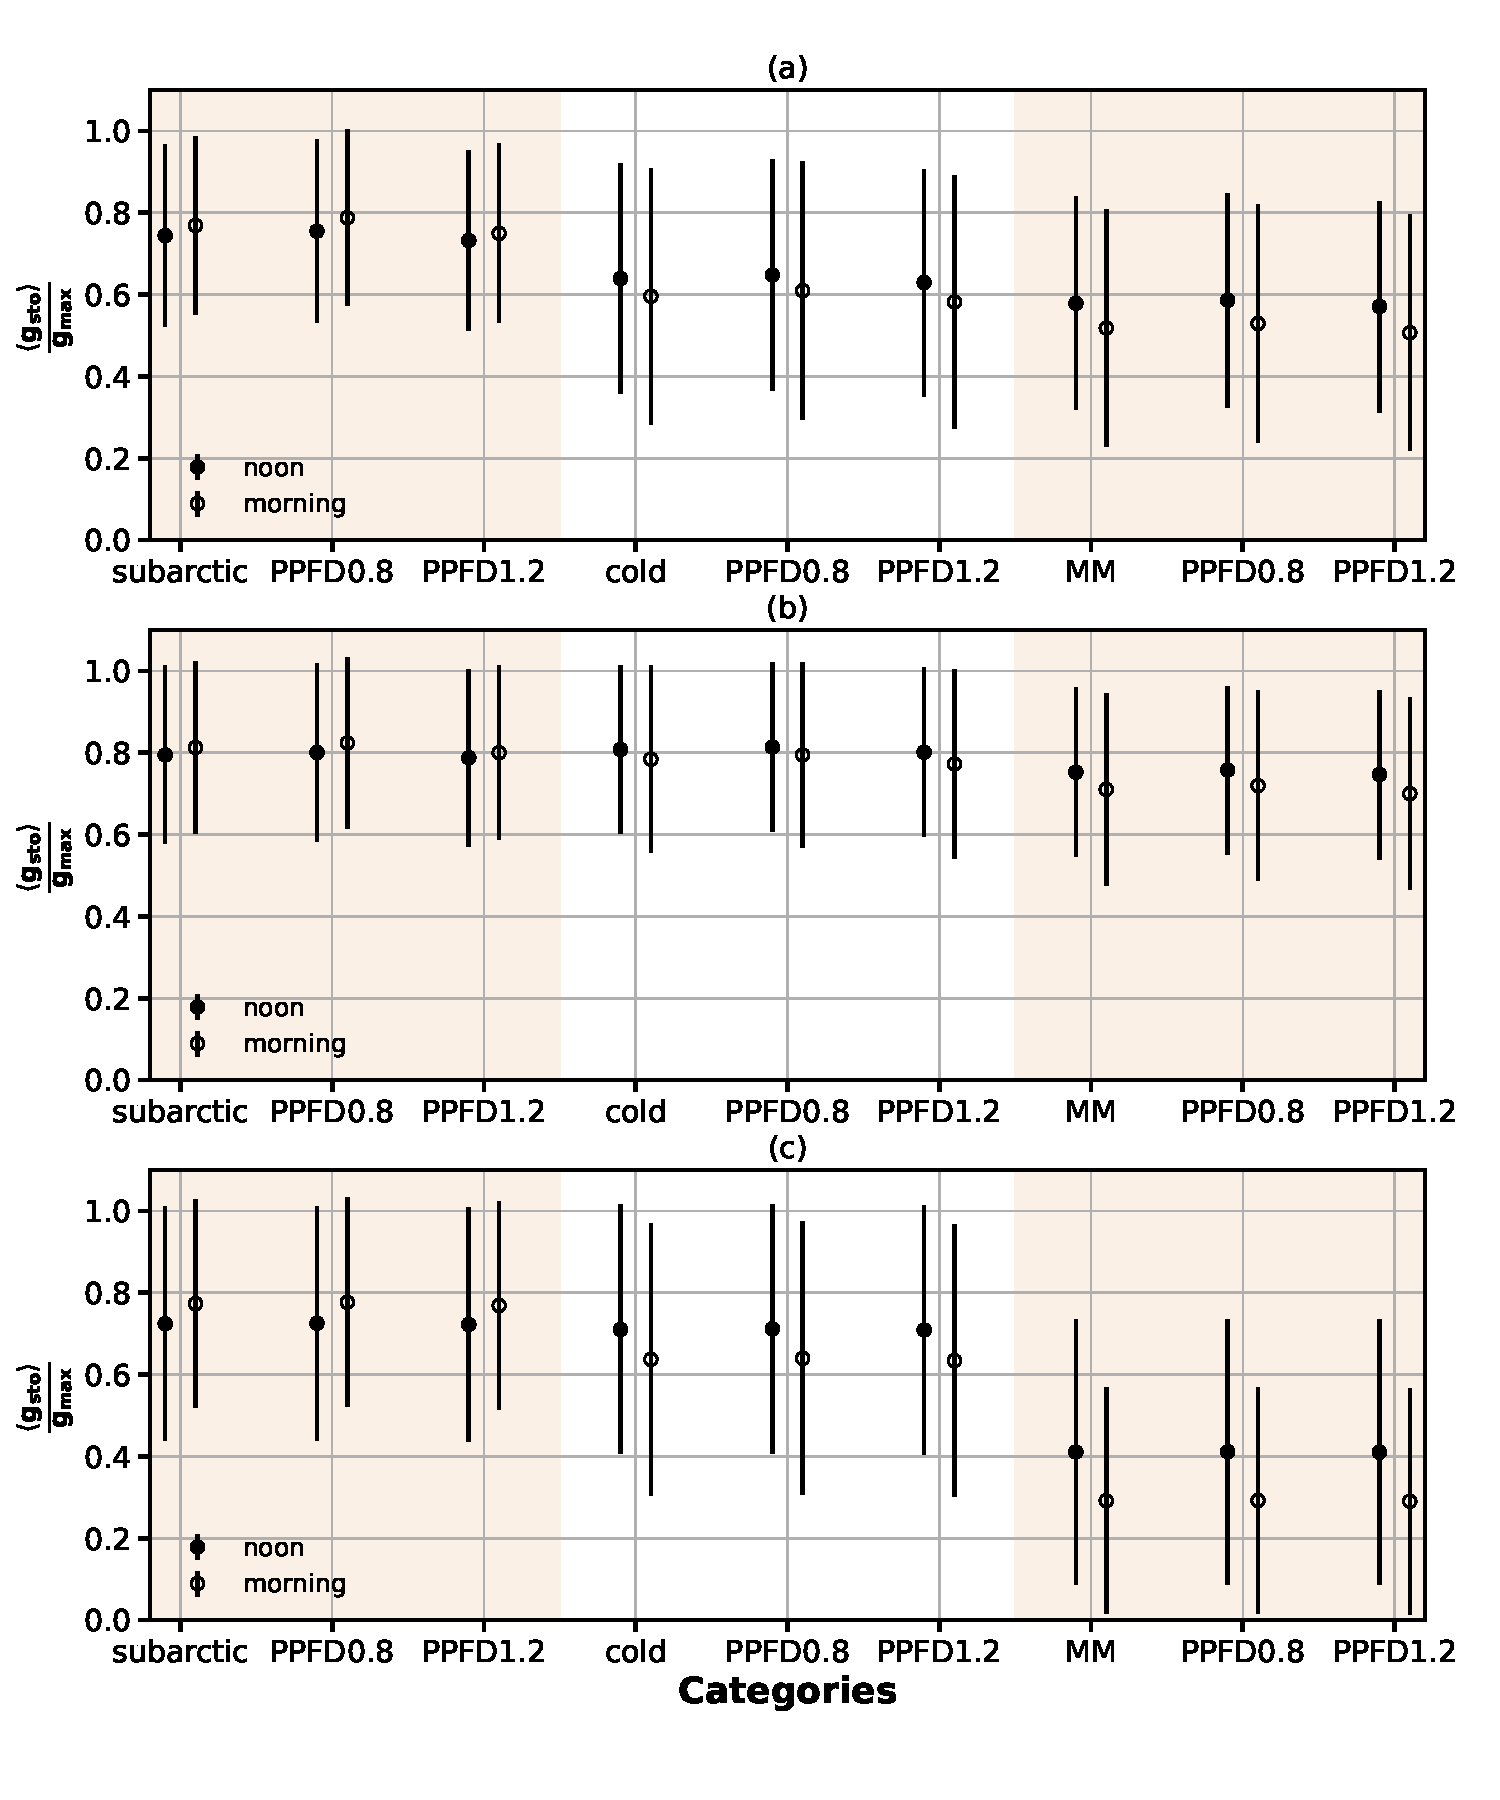
\includegraphics[width=8.3cm]{javis_func_opt_mean.pdf}
  \caption{Proposed metric to test bespoke response functions.}
  \label{fig:javis_func_opt_mean}
\end{figure}

Start ($A_\text{start}$) and end ($A_\text{end}$) of growing season for each PFT are given in units of day of year (doy) and estimated as follows. Evergreen needle leaf trees are photosynthetic active already at low temperatures \citep{TB:Kolari2007}. This leads necessarily to an increase in observable net photosynthesis. Hence, we use a MODIS (Aqua/Terra) retrieved net photosynthesis product for a $1\times 1\,\unit{km}$ patch centered at Svanhovd to determine onset and end of growing season. Net photosynthesis data can be approximated by a second order polynomial function (Fig.~\ref{fig:modis_Psn}). By calculating the roots of the fitted polynomial, we derive $A_\text{start} = 122\,\unit{doy}$ for 2018 and day 106 in 2019. $A_\text{end}$ amounts to day 261 and 274, respectively, and shall be used for all vegetation alike. The resulting growing season for Norway spruce in 2019 was one month longer then in 2018. For estimating $A_\text{start}$ of birch tree, we use the $5$ consecutive days above $5\,\unit{^\circ C}$ agricultural rule of thumb on gridded temperature data from SeNorge.no (Fig.~\ref{fig:greening_season_change_Svanvik}). We find 129 and 130, respectively. From the latitude model typically used for localizing $\mathrm{DO_3SE}$, we get $A_\mathrm{start} = 100\,\unit{doy}$ and $A_\mathrm{end} = 307\,\unit{doy}$ indicating an about $2\,\unit{months}$ longer growing season. For perennial grassland, we assume a latency period of about $1\,\unit{month}$ after snow melt. Data for first snow-free day is taken from the weather station at Øvre Neiden in Sør-Varanger. In both years, the first snow-free day incidents with the estimated date of bud burst. As leafs of birches in northern Fennoscandia \emph{Betula pubescens} are smaller than southern specimen, we have measured their dimension for the purpose of this study and find $(3.0\pm 0.5)\,\unit{cm}$. \citet[][p.~52]{NINA2004} indicate an average tree height of $13.5\,\unit{m}$ in the area.

As pointed out by \citet{ACP:Bueker2012}, a very important factor in deriving a proper $\mathrm{POD_y}$ is the soil texture or how much water the soil can hold. As Svanhovd is located in the bed of the Pasvik river, we assume a sandy loam texture at $60\,\unit{cm}$ depth.\\



\subsection{POD and ozone impact}

We have modeled $\mathrm{POD_y}$ for three natural/semi-natural vegetation PFTs, birch, Norway spruce, and perennial grassland. The results are shown comprehensively in Fig.~\ref{fig:pody} as a function of doy for March--October. A flux threshold $y=1\,\unit{nmol\,m^{-2}\,s^{-1}}$ per projected leaf area (PLA) has been chosen. \chem{[O_3]} are plotted on the same axis and scales as $G_\text{sto}^\text{leaf}$ but in units of $\unit{ppb}$.

As expected, $\mathrm{POD_y}$ is higher in 2018 than in 2019 for all PFTs. In the end of the 2018 season, Birch took up $13.1\,\unit{mmol\,m^{-2}\,PLA}$, while perennial grassland had an uptake of $4.5\,\unit{mmol\,m^{-2}\,PLA}$. The largest interannual variation is also found in Birch ($2.1\,\unit{mmol\,m^{-2}\,PLA}$) and perennial grassland ($2.6\,\unit{mmol\,m^{-2}\,PLA}$). Whereas, there is only a small difference for Norway spruce ($0.3\,\unit{mmol\,m^{-2}\,PLA}$) between the two years.

%Except for perennial grassland, model integrations with climatological forcings show higher $\mathrm{POD_y}$ than 2018. This can be explained by means of non linearity in modeled stomatal conductance (Eq.~(\ref{eq:stomatal})) in Eq.~(\ref{eq:pod}). The climatology in $\mathrm{POD_y}$ therefore represents rather an ideal year for growth then a true climatology. To establish a true climatology, it would be necessary to run the $\mathrm{DO_3SE}$ model for 10--20 years with respective observed phenology as well as meteorological and ozone forcing. 

%Based on this interpretation of climatology in $\mathrm{POD_y}$, we can learn more about potential ozone damage. The time derivative $\frac{\mathrm{\Delta POD_y}}{\Delta t}$ displays very different features for each PFT and meteorological forcing. Although Norway spruce shows a low interannual variation, $\frac{\mathrm{\Delta POD_y}}{\Delta t}$ (Fig.~\ref{fig:pody_rel}) indicates an extended period of higher than average ozone uptake in spring 2018 (steep slope), while ozone uptake in June/July was anomalously low in 2019 (shallow slope) but high in fall. This is most prominently visible in Fig.~\ref{fig:pody}h) for perennial grassland, where consecutive periods of low $G_\text{sto}^\text{leaf}$ manifest in three plateaus in $\mathrm{POD_y}$ throughout the season (1: $184-198\,\unit{doy}$, 2: $209-228\,\unit{doy}$, 3: $235-240\,\unit{doy}$). An episode with anomalous high ozone in mid June ($194\,\unit{doy}$) can be identified but does not amount to unusually high ozone uptake on an annual basis.

The estimated biomass reduction in \unit{\%} due to \chem{O_3} following \citet{ICP:MappingManual2017} is shown in Table~\ref{tab:biomass_reduction}. {\bf TODO: Lisa? Add paragraph about biomass reduction to introduction?}

\begin{figure*}[t]
  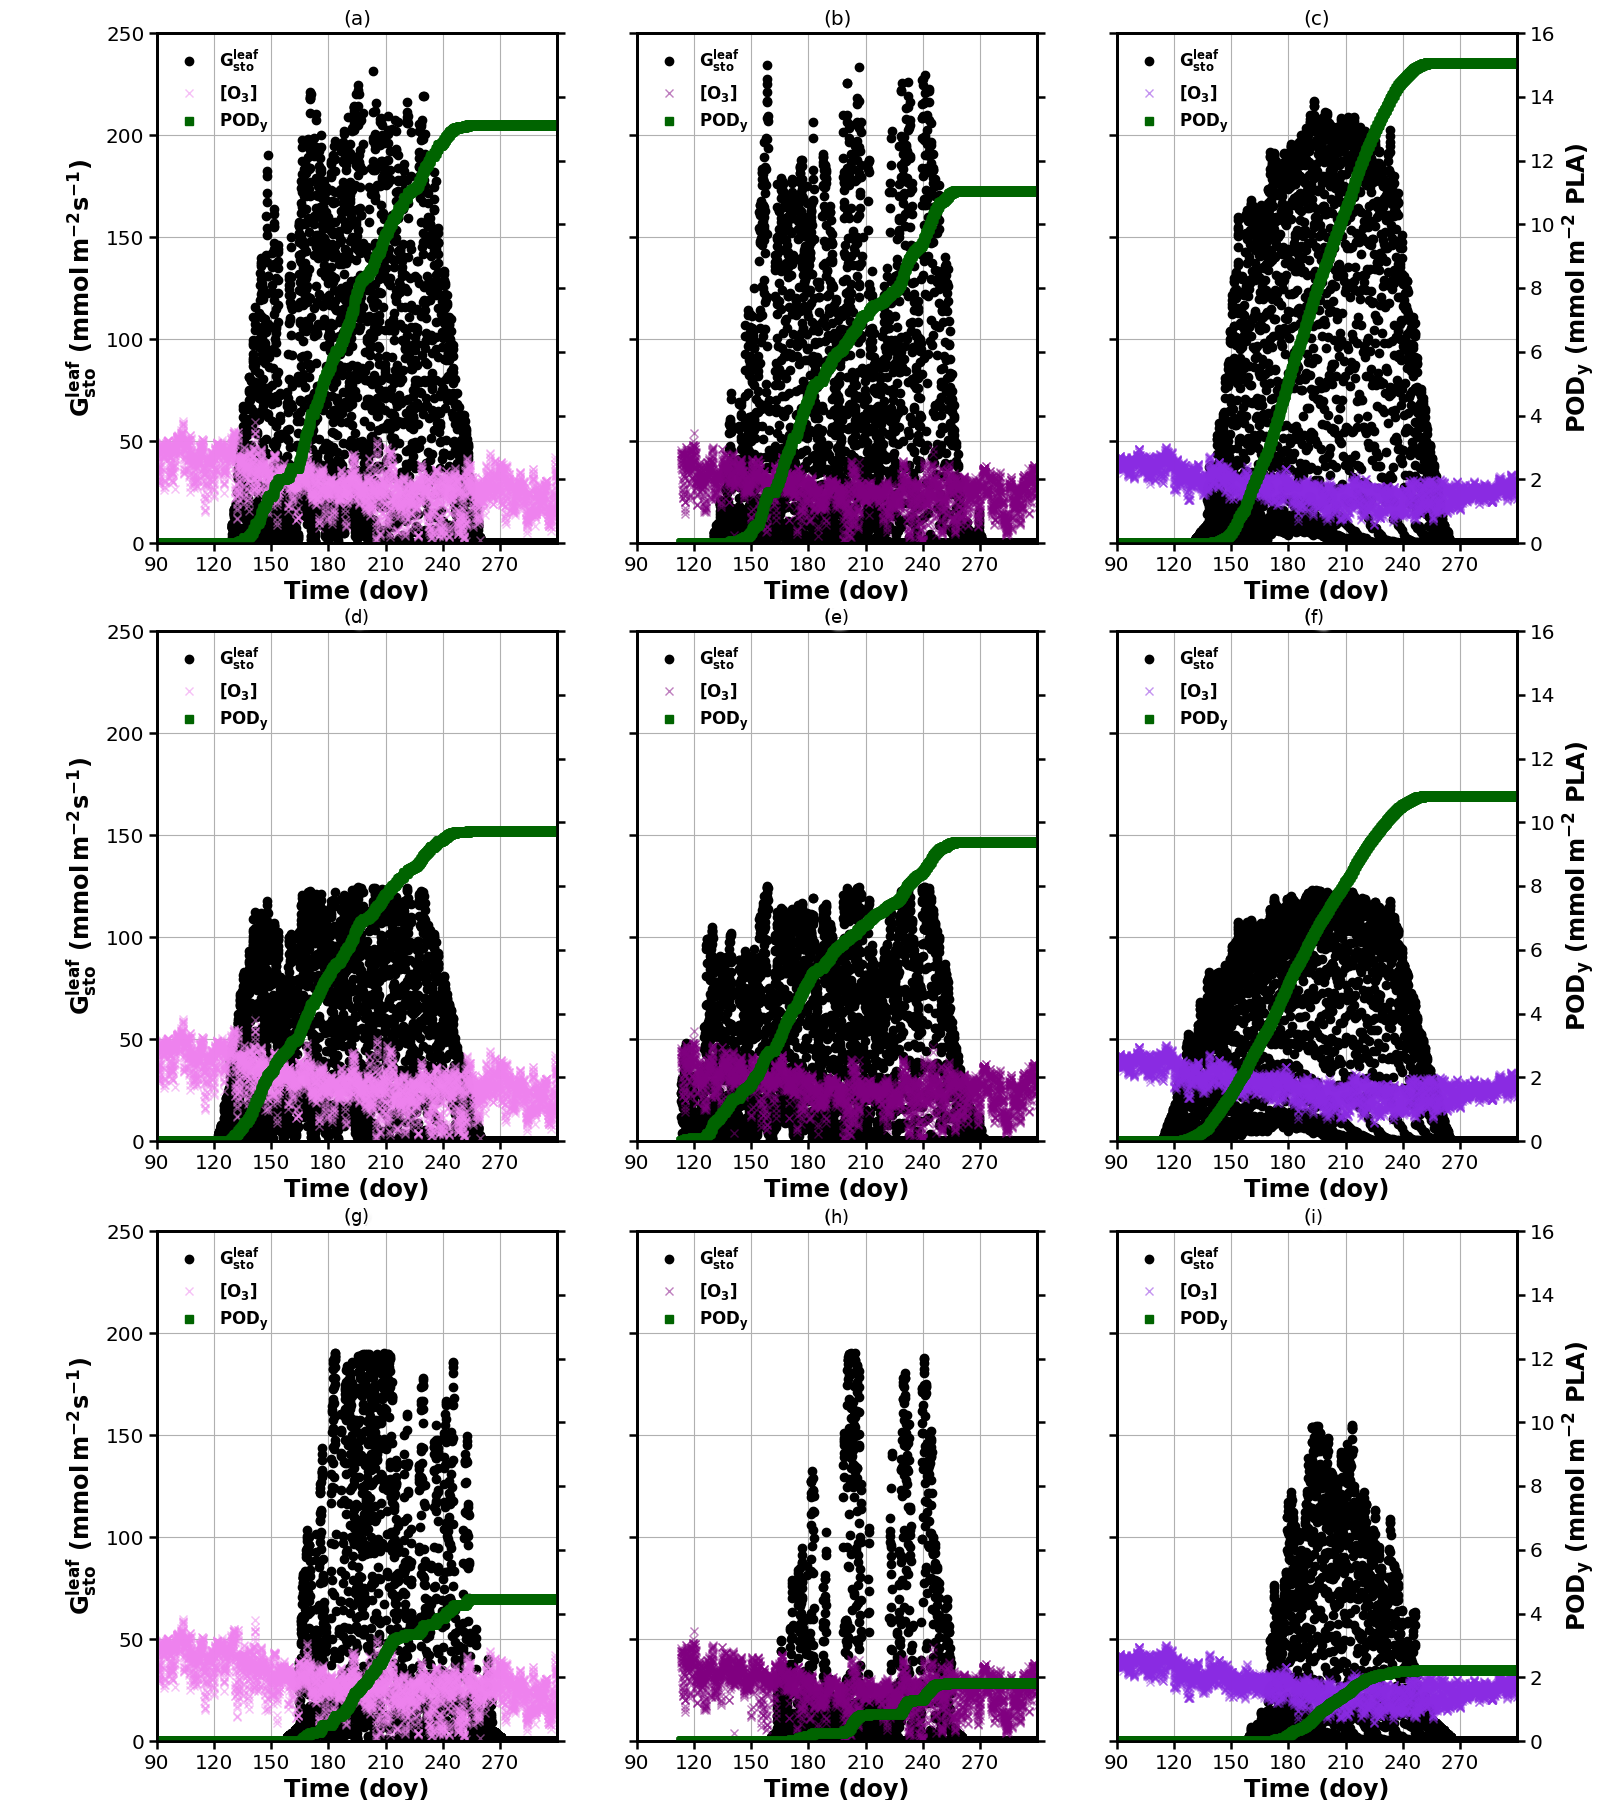
\includegraphics[width=12cm]{DO3SE_results_pody_gsto_o3}
  \caption{$\mathrm{POD_y}$ modeling results from $\mathrm{DO_3SE}$ model for three different PFTs over day of year (doy), March--October. A flux threshold $y=1\,\unit{nmol\,m^{-2}\,s^{-1}}$ per projected leaf area (PLA) has been chosen. \chem{[O_3]} are plotted on the same axis and scales as $G_\text{sto}^\text{leaf}$ but in units of $\unit{ppb}$. (a, b) Birch; (c, d) Norway spruce; (e, f) perennial grassland. From left to right: 2018, 2019. {\bf TODO: substitute with figure for boreal PFTs?}}
  \label{fig:pody}
\end{figure*}


\begin{table}[t]
  \caption{Estimated total biomass reduction in \unit{\%} due to \chem{O_3} following \citet{ICP:MappingManual2017}.}
  \label{tab:biomass_reduction}
\begin{tabular}{lccrr}
\tophline
Year & \multicolumn{4}{c}{PFT}\\
& Birch & Norway spruce & \multicolumn{2}{c}{Perennial grassland}\\
\middlehline
2018 & 11.99 & 2.34 & 8.06 & 10.51$^*$\\
2019 & 10.07 & 2.26 & 6.43 & 7.90$^*$\\
clim. & 13.81 & 2.58 & 6.67 & 8.29$^*$\\
\bottomhline
\end{tabular}
\belowtable{$^*$ above ground biomass} % Table Footnotes
\end{table}

%\begin{figure}[t]
%  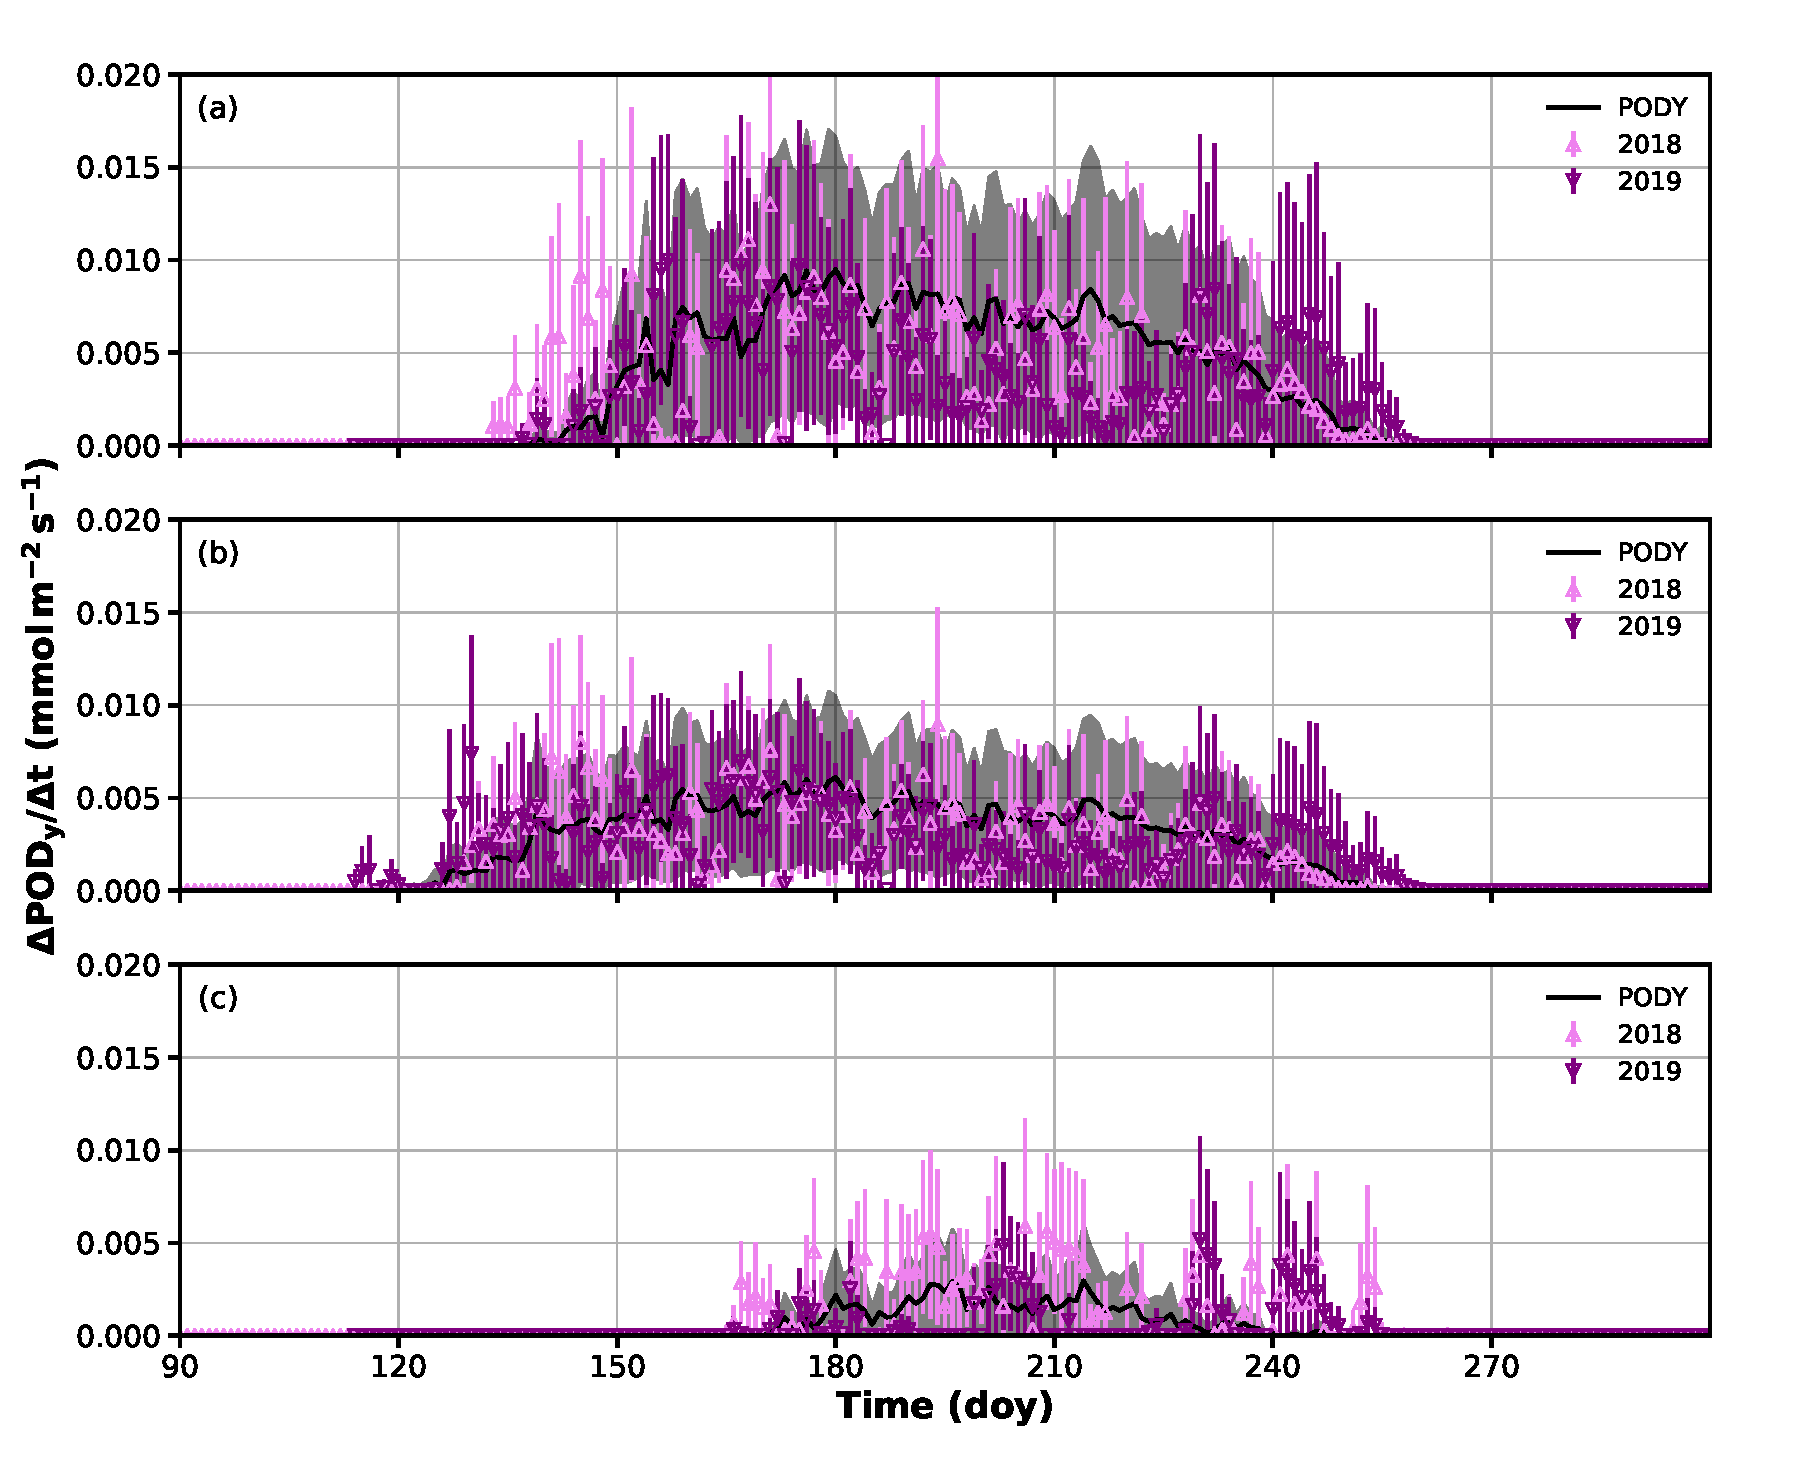
\includegraphics[width=8.3cm]{DO3SE_results_rel}
%  \caption{Daily averaged $\mathrm{\Delta POD_y}/\Delta t$ from $\mathrm{DO_3SE}$ model for three different PFTs over day of year (doy), March--October. Error bars/-bands indicate $1 \sigma$ standard deviation. (a) Birch; (b) Norway spruce; (c) perennial grassland.}
%  \label{fig:pody_rel}
%\end{figure}

\conclusions[Discussion and conclusions]
\label{sec:conc} 
\begin{itemize}
  \item What did we learn from the 2018/2019 seasons in terms of ozone damage in the far north?
  \item What are the main uncertainties in the tools we've used?
  \item What implications could this have for future scenarios in which 2018 conditions may occur more often?
\end{itemize}
PODY is no good measure without a damage function with higher temporal resolution than annual. This has been already pointed out by \citet{AE:Musselman2006}! Higher than normal spring uptake (weather conditions) does not amount to critical uptake on an annual basis. 
Weather and climatic conditioning of plants is more important for PODy than episodes of higher than usual ozone concentrations. Therefor high $\Delta \mathrm{POD_y} / \Delta t$ is not accounted for properly.
It is important to know the plant response functions to temperature, light, humidity/precipitation as best as possible if one wants to assess risk of damage.

Regarding the shift (earlier) and prolongation (later) of the growing season in the far north no general assessment can be made. Data show that in both 2018 and 2019 ozone uptake in early season was anomalous high in all studied PFTs. The extended growing season in 2019 might have countered higher episodic ozone uptake in 2018. In both years, low mid-season uptake due to weather conditions washed out any effect of these.

{\bf TODO: might be interesting to look at Mills et al 2003 and the different spatial extents of risk estimated when using AOT40 vs PODy. That could be useful to explain why we focus on PODy (rather then AOT40).- Lisa Come back to this later on in the discussions(?) - it has not been breached at Svanvik in northern Fennoscandia.}

Bigger picture:
\begin{itemize}
\item Ozone damage assessment using mapping manual "compromise" parameterization.
\item Land-atmosphere modelling: Problems in productivity of species especially in the arctic regions due to PFTs which are not suited for the climate. Automating optimization of climate adaption of general PFTs.
\end{itemize}

%% The following commands are for the statements about the availability of data sets and/or software code corresponding to the manuscript.
%% It is strongly recommended to make use of these sections in case data sets and/or software code have been part of your research the article is based on.

%\codeavailability{TEXT} %% use this section when having only software code available


\dataavailability{TEXT} %% use this section when having only data sets available


%\codedataavailability{TEXT} %% use this section when having data sets and software code available


\sampleavailability{TEXT} %% use this section when having geoscientific samples available


%\videosupplement{TEXT} %% use this section when having video supplements available


\appendix
\section{Derived climatologies}    %% Appendix A

\subsection{Temperature, precipitation, and global irradiance}     %% Appendix A1, A2, etc.

\appendixfigures  %% needs to be added in front of appendix figures
\begin{figure*}[t]
  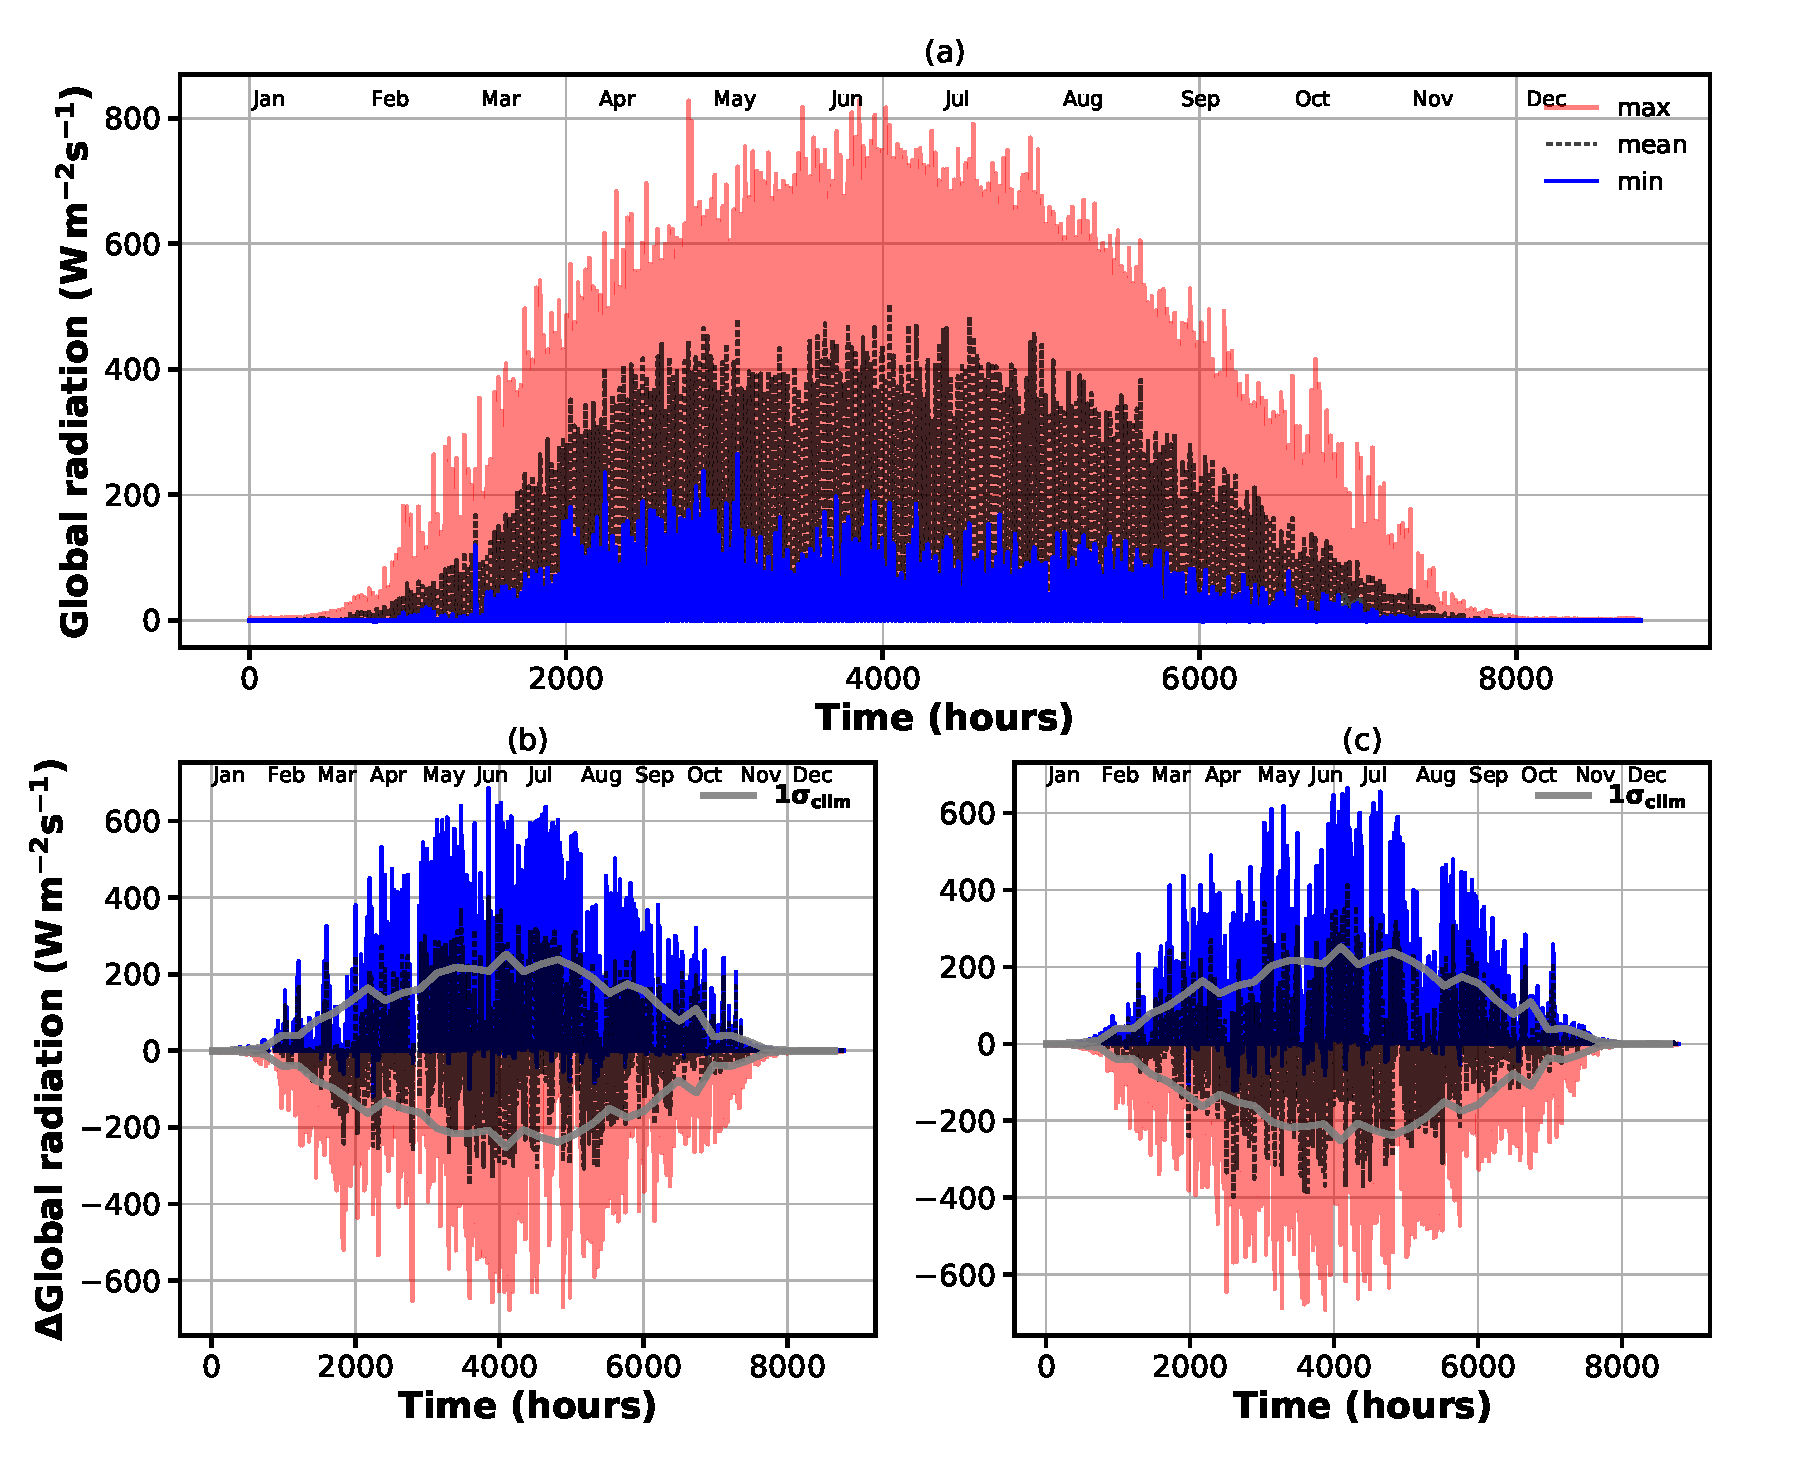
\includegraphics[width=12cm]{global_rad_clim}
  \caption{Observed global irradiance at Svanvik. The cyan lines indicate the $1\,\sigma$ level deducted from the climatology. (a) Climatology (hourly maxima, mean, and minima); deviation from climatology (b) 2018; (c) 2019.}
  \label{fig:global_rad_clim}
\end{figure*}

\begin{figure*}[t]
  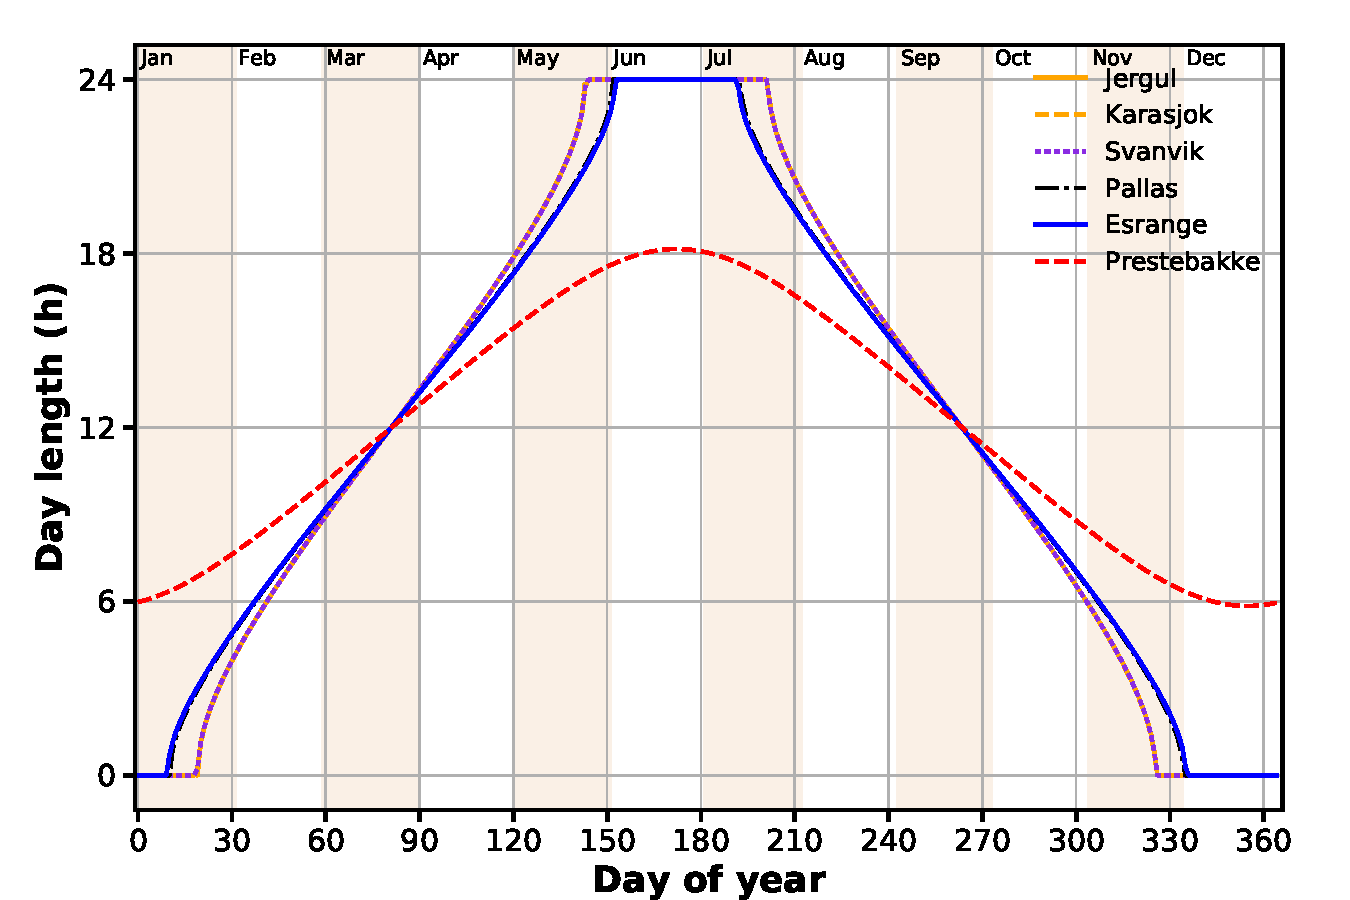
\includegraphics[width=12cm]{test_fennoscandia}
  \caption{Maximum daily sun shine duration based on geometrical calculations at different sites in Fennoscandia. Midnight sun conditions at Jergul/Karasjok and Svanvik prevail from the end of May until the end of July, while at Esrange and Pallas they only prevail from the beginning of June until mid of July.}
  \label{fig:sunlight_fennoscandia}
\end{figure*}

\begin{figure*}[t]
  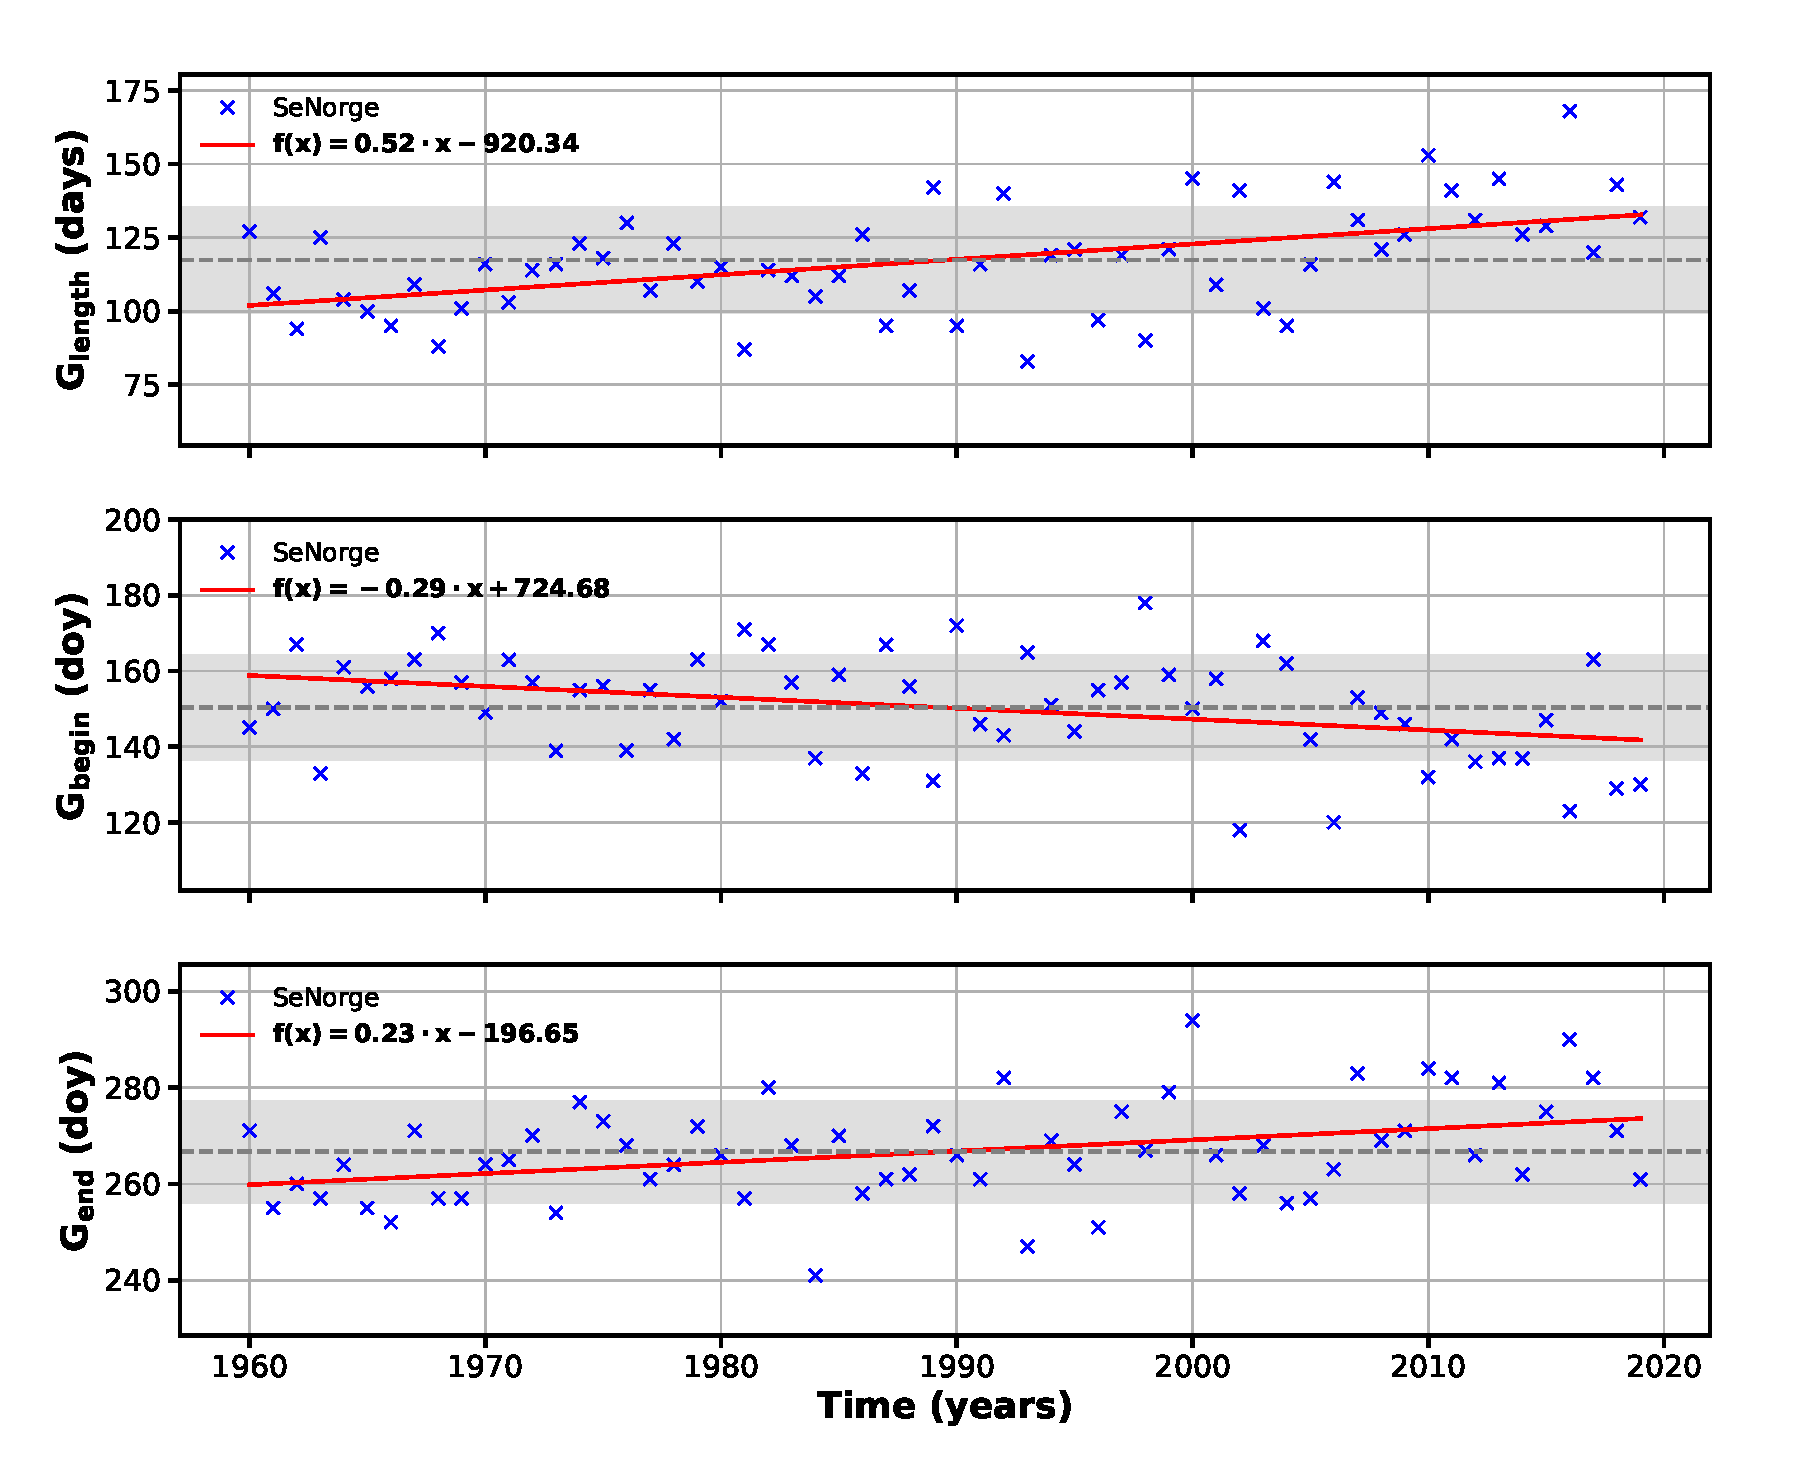
\includegraphics[width=12cm]{greening_season_change_Svanvik}
  \caption{Estimated shift and prolongation of greening season at Svanhovd over the past 6 decades based on data from SeNorge.no {\bf TODO: citation http://www.senorge.no}.}
  \label{fig:greening_season_change_Svanvik}
\end{figure*}
\clearpage


\subsection{Ozone}

\begin{figure*}[t]
  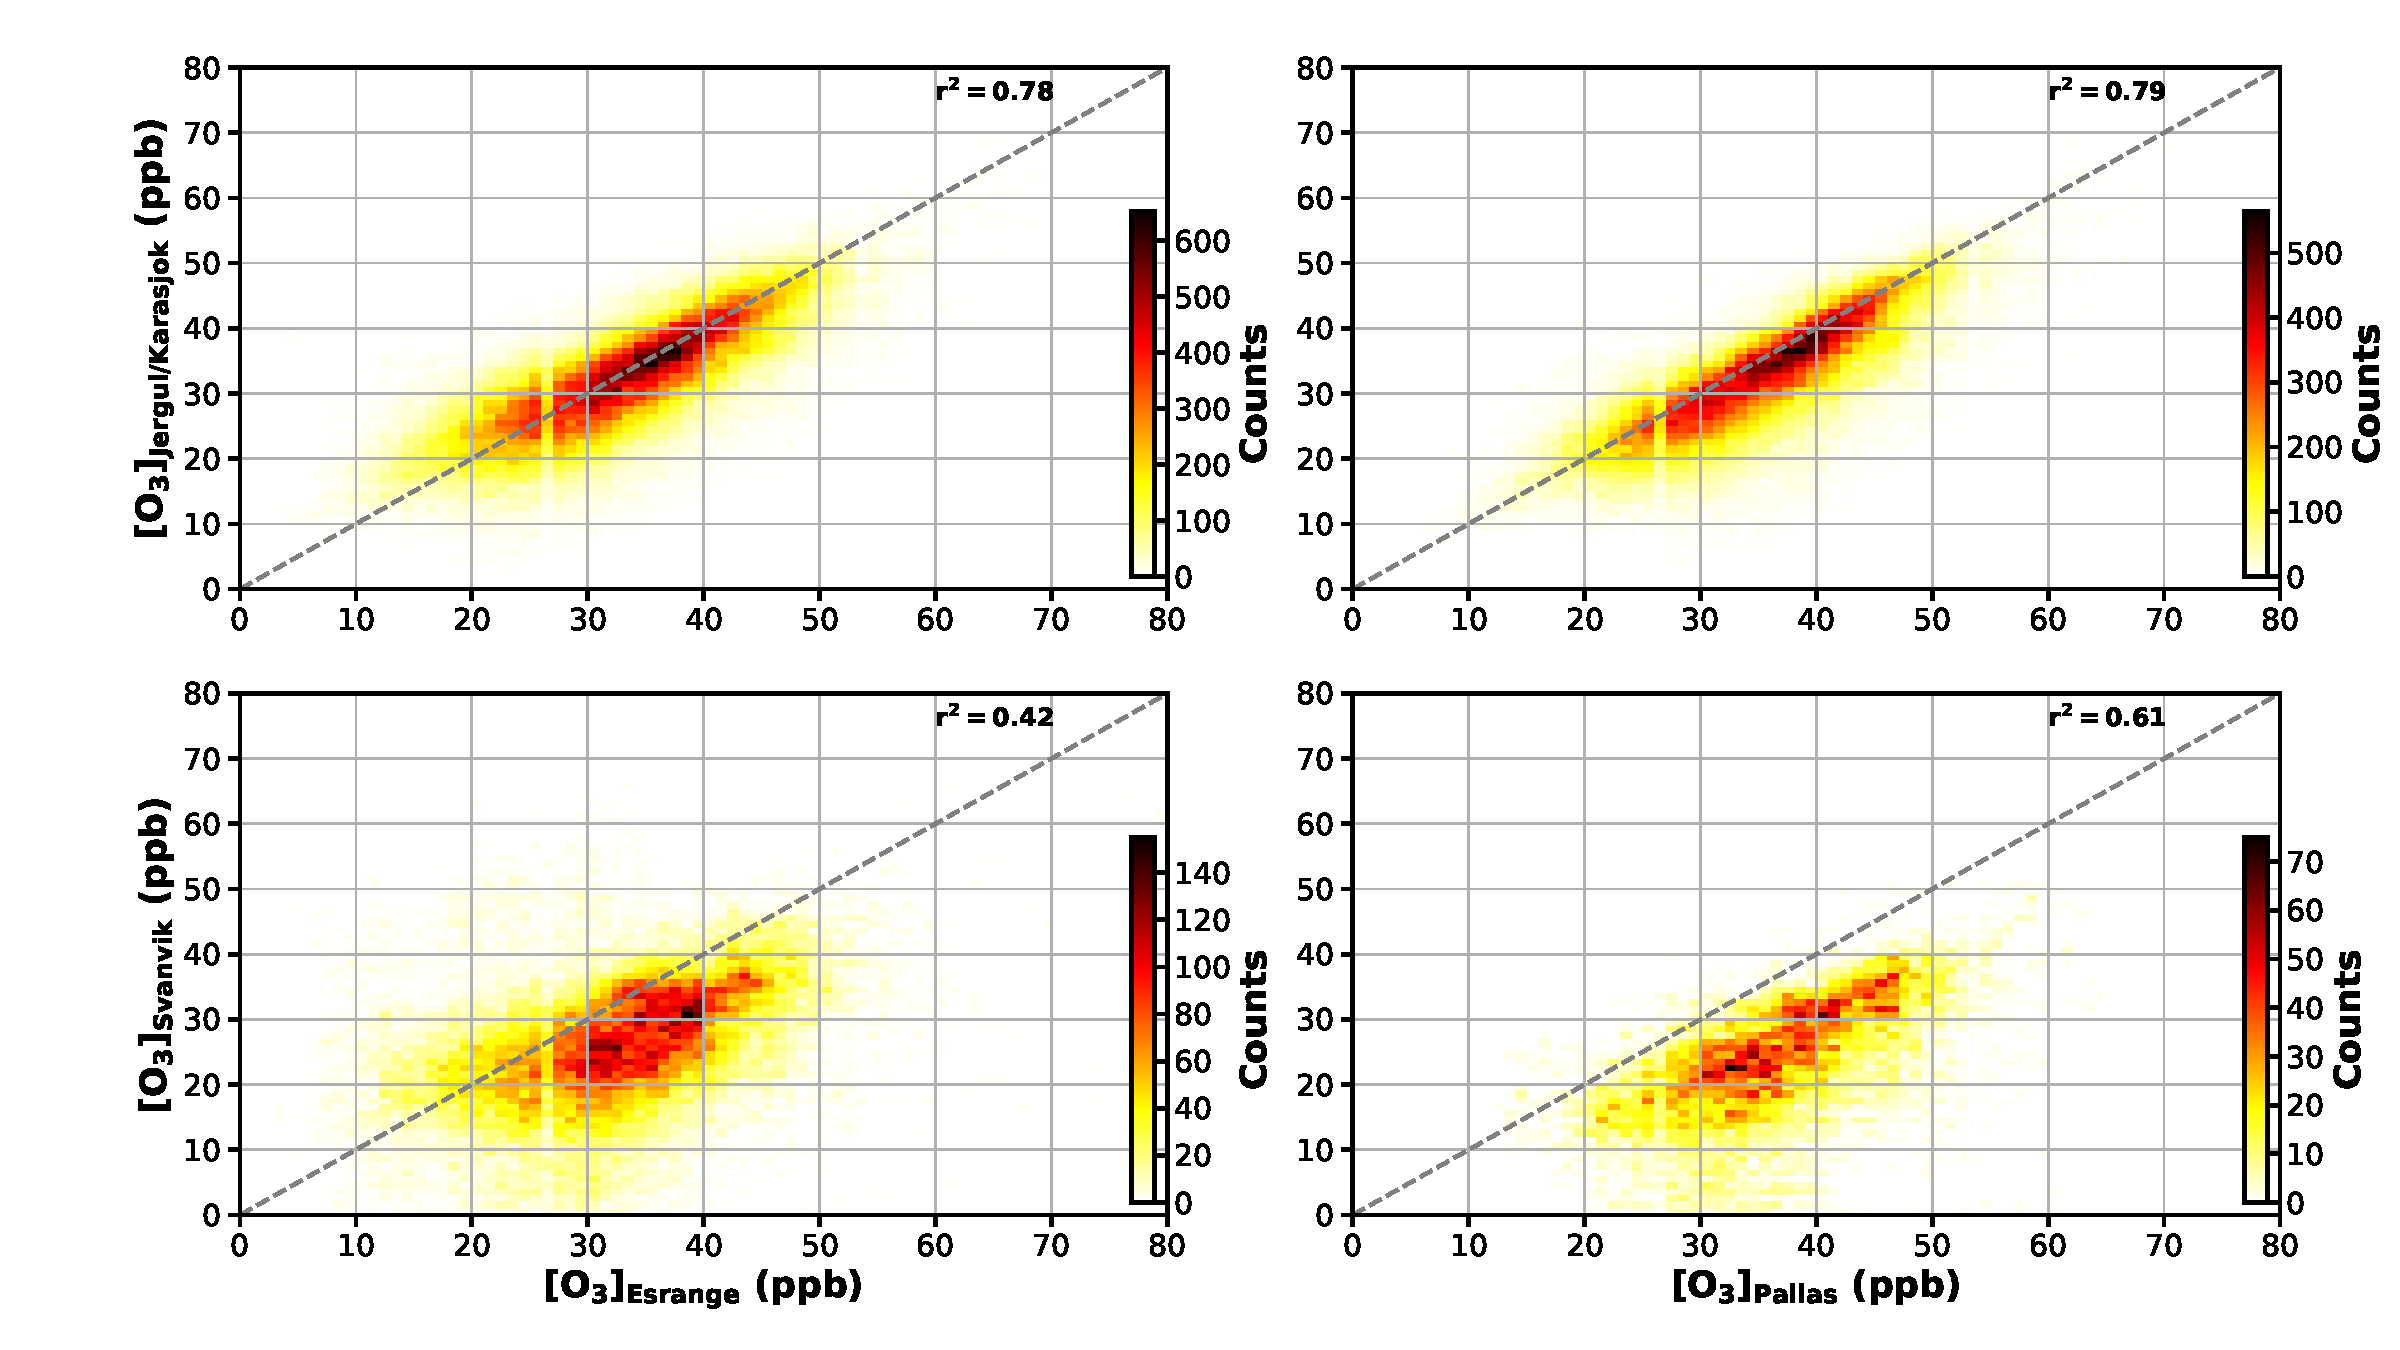
\includegraphics[width=12cm]{density_distribution}
  \caption{Probability densities and correlation coefficient for \chem{[O_3]} between different sites in northern Fennoscandia. Jergul/Karasjok is well correlated with Esrange, and Pallas. Svanvik displays highest correlation with Pallas. (a) Jergul/Karasjok--Esrange; (b) Jergul/Karasjok--Pallas; (c) Svanvik--Esrange; (d) Svanvik--Pallas.}
  \label{fig:density_distribution}
\end{figure*}

\begin{figure*}[t]
  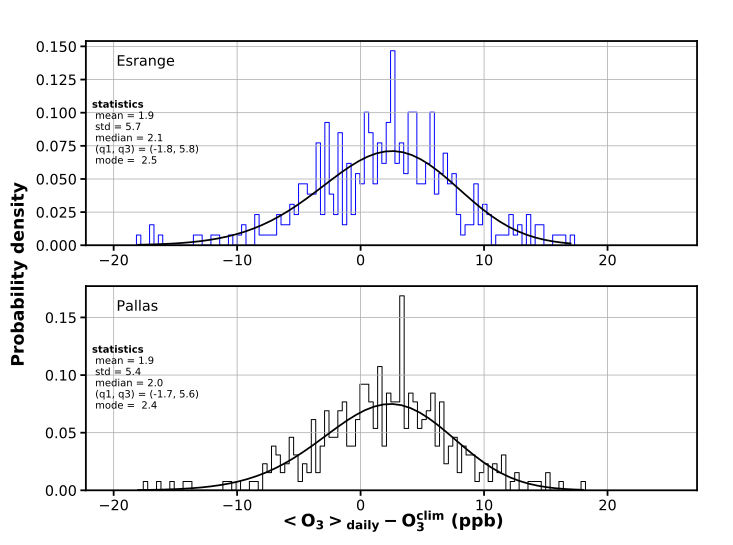
\includegraphics[width=12cm]{ozone_climatology_fenoscandic_obs_residuals}
  \caption{Probability density functions of ozone concentration residuals. 2018 with respect to respective climatology for different sites in Fennoscandia. (a) Esrange; (b) Pallas.}
  \label{fig:ozone_climatology_fenoscandic_obs_residuals}
\end{figure*}

\begin{figure*}[t]
  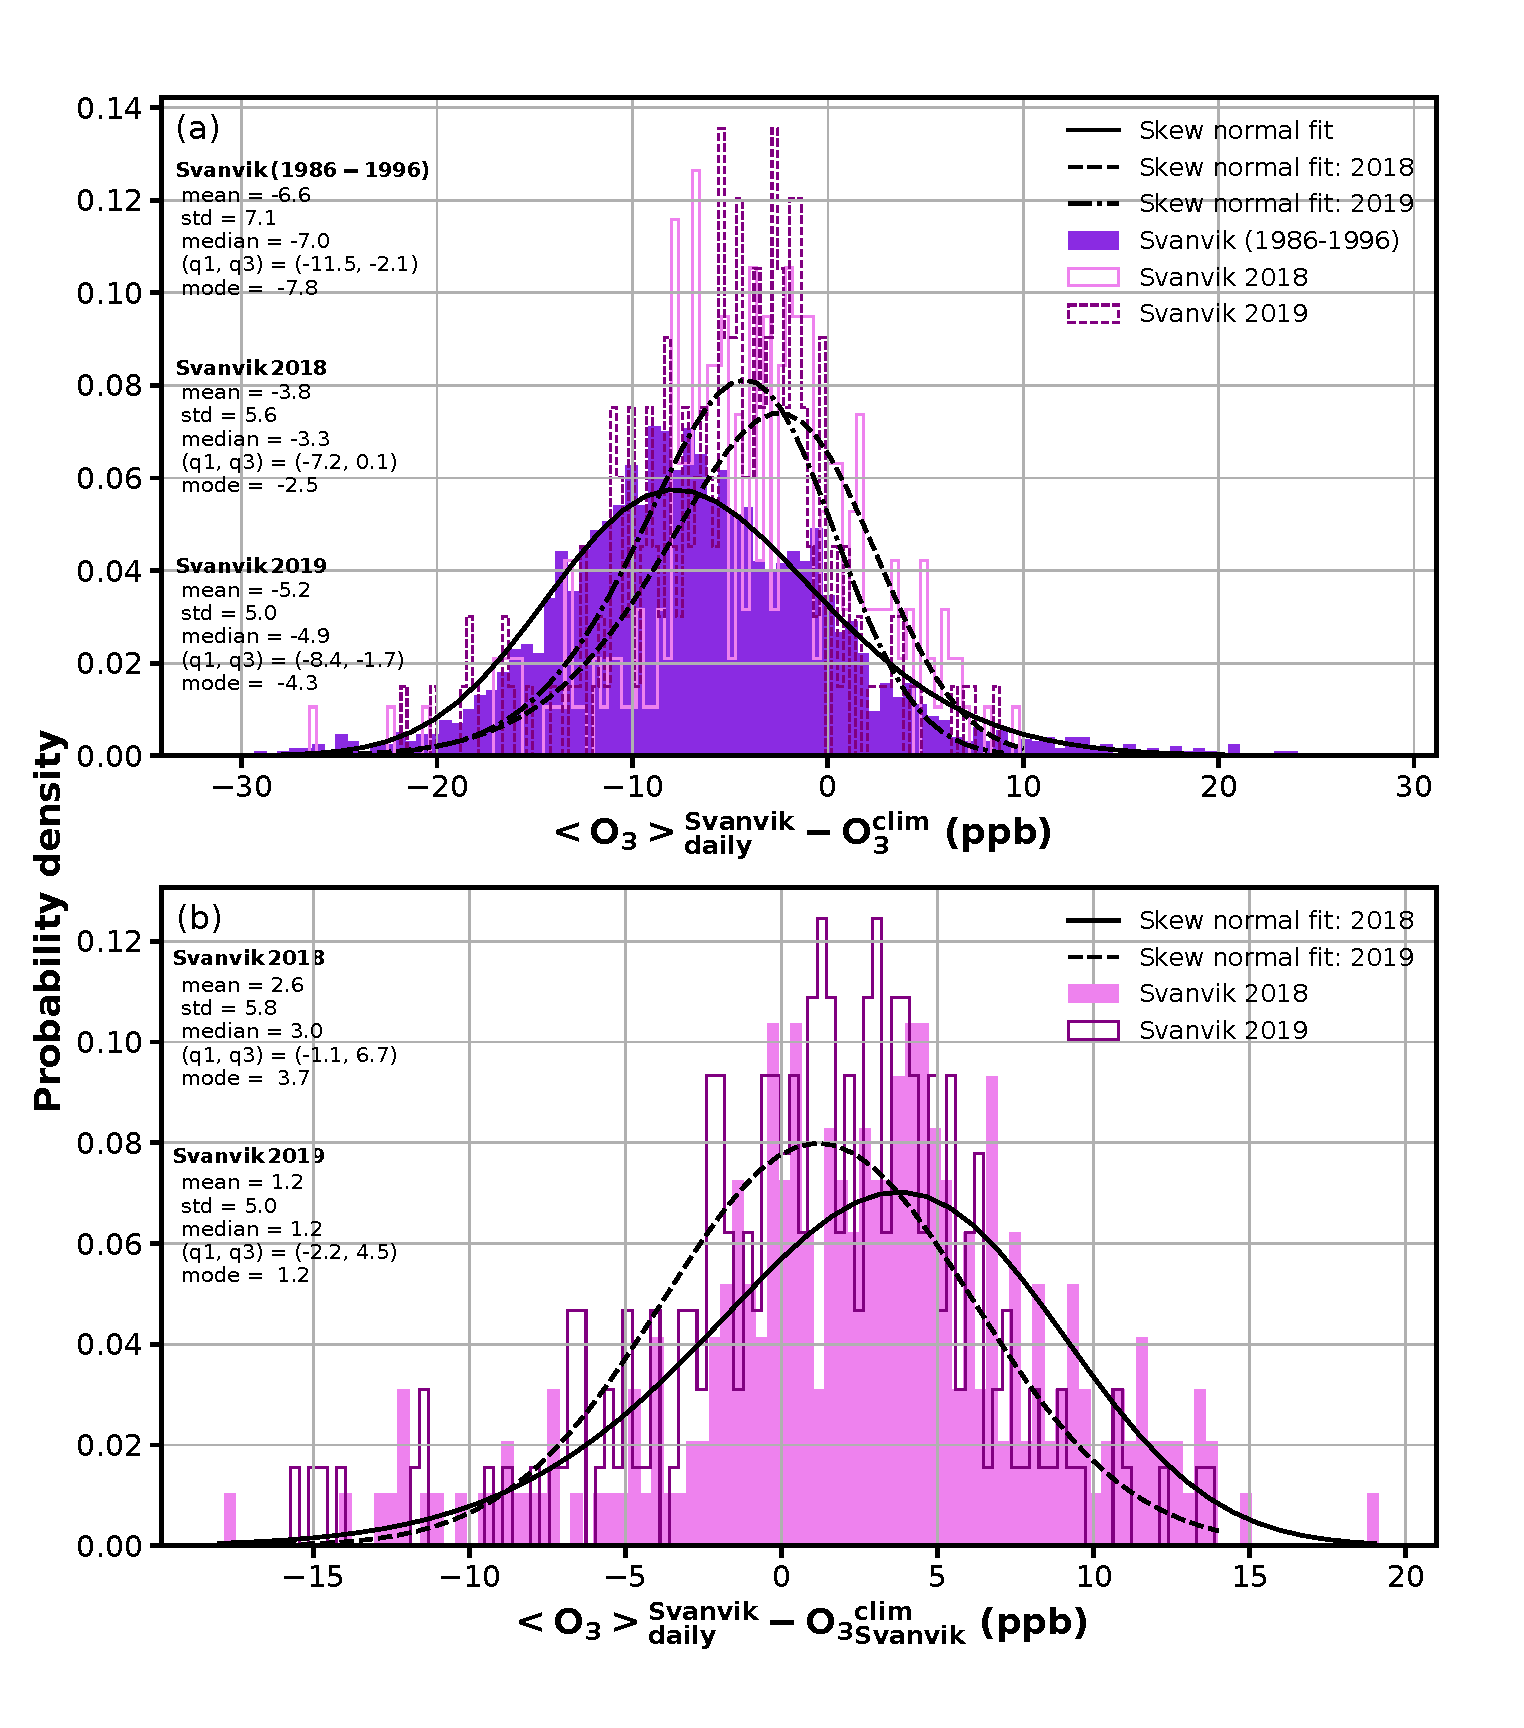
\includegraphics[width=12cm]{ozone_climatology_fenoscandic_obs_residuals-Svanvik}
  \caption{Probability density functions of ozone concentration residuals. 2018/19 observations at Svanhovd with respect to derived climatologies for (a) Northern Fennoscandia; (b) Svanvik.}
  \label{fig:ozone_climatology_fenoscandic_obs_residuals-Svanvik}
\end{figure*}

\begin{figure*}[t]
  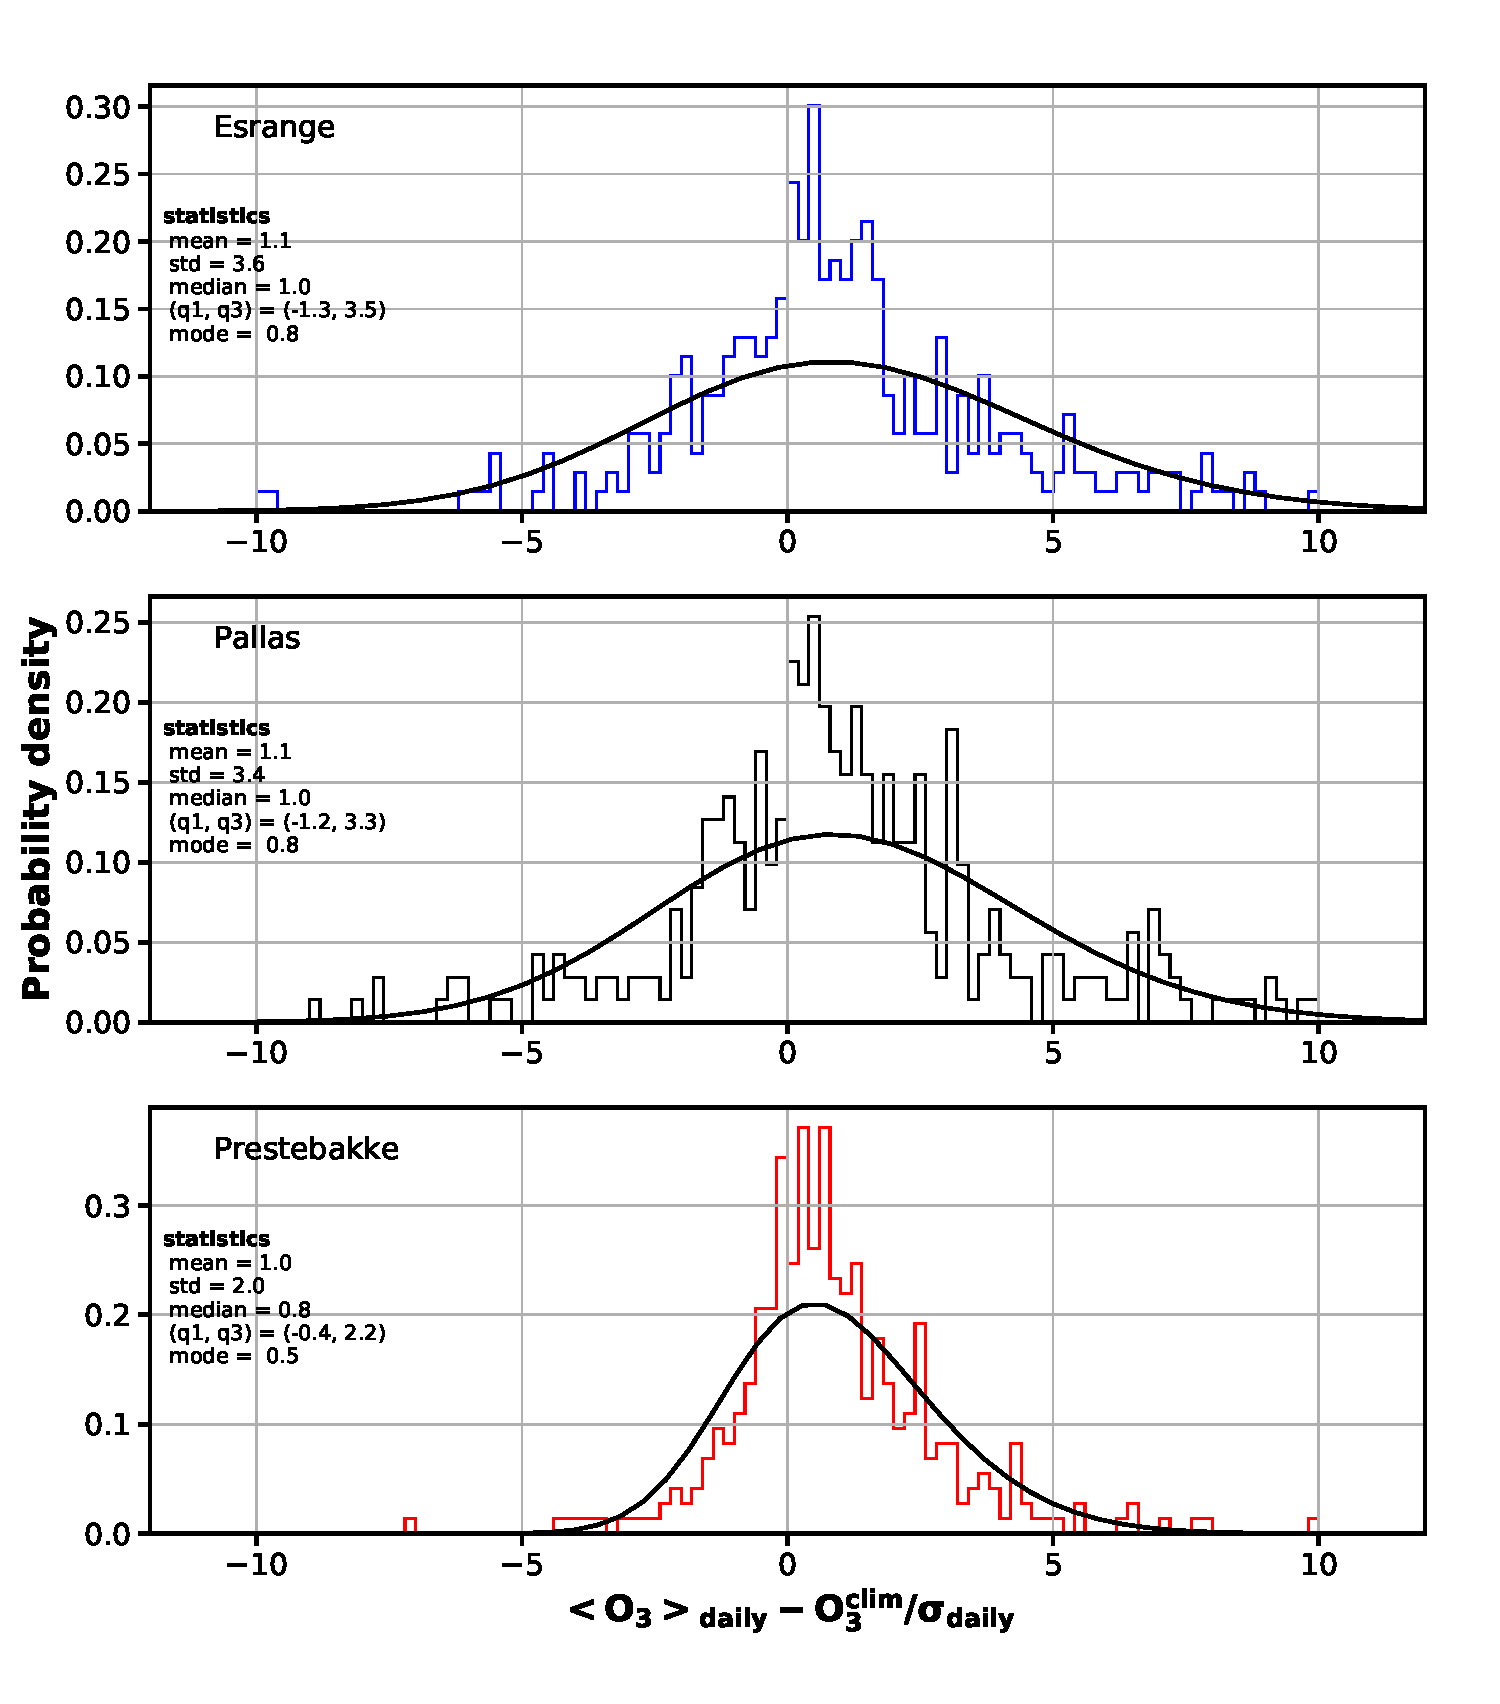
\includegraphics[width=12cm]{ozone_climatology_fenoscandic_obs_test}
  \caption{Student's t-test assuming same sample uncertainty in both, climatology and 2018 observations for different sites in Fennoscandia. \chem{\Delta[O_3]} in Fig.~\ref{fig:ozone_climatology_fenoscandic_obs_residuals} are significantly different from zero-hypothesis on the $1\,\sigma$ level. (a) Esrange; (b) Pallas.}
  \label{fig:ozone_climatology_fenoscandic_obs_test}
\end{figure*}

\begin{figure*}[t]
  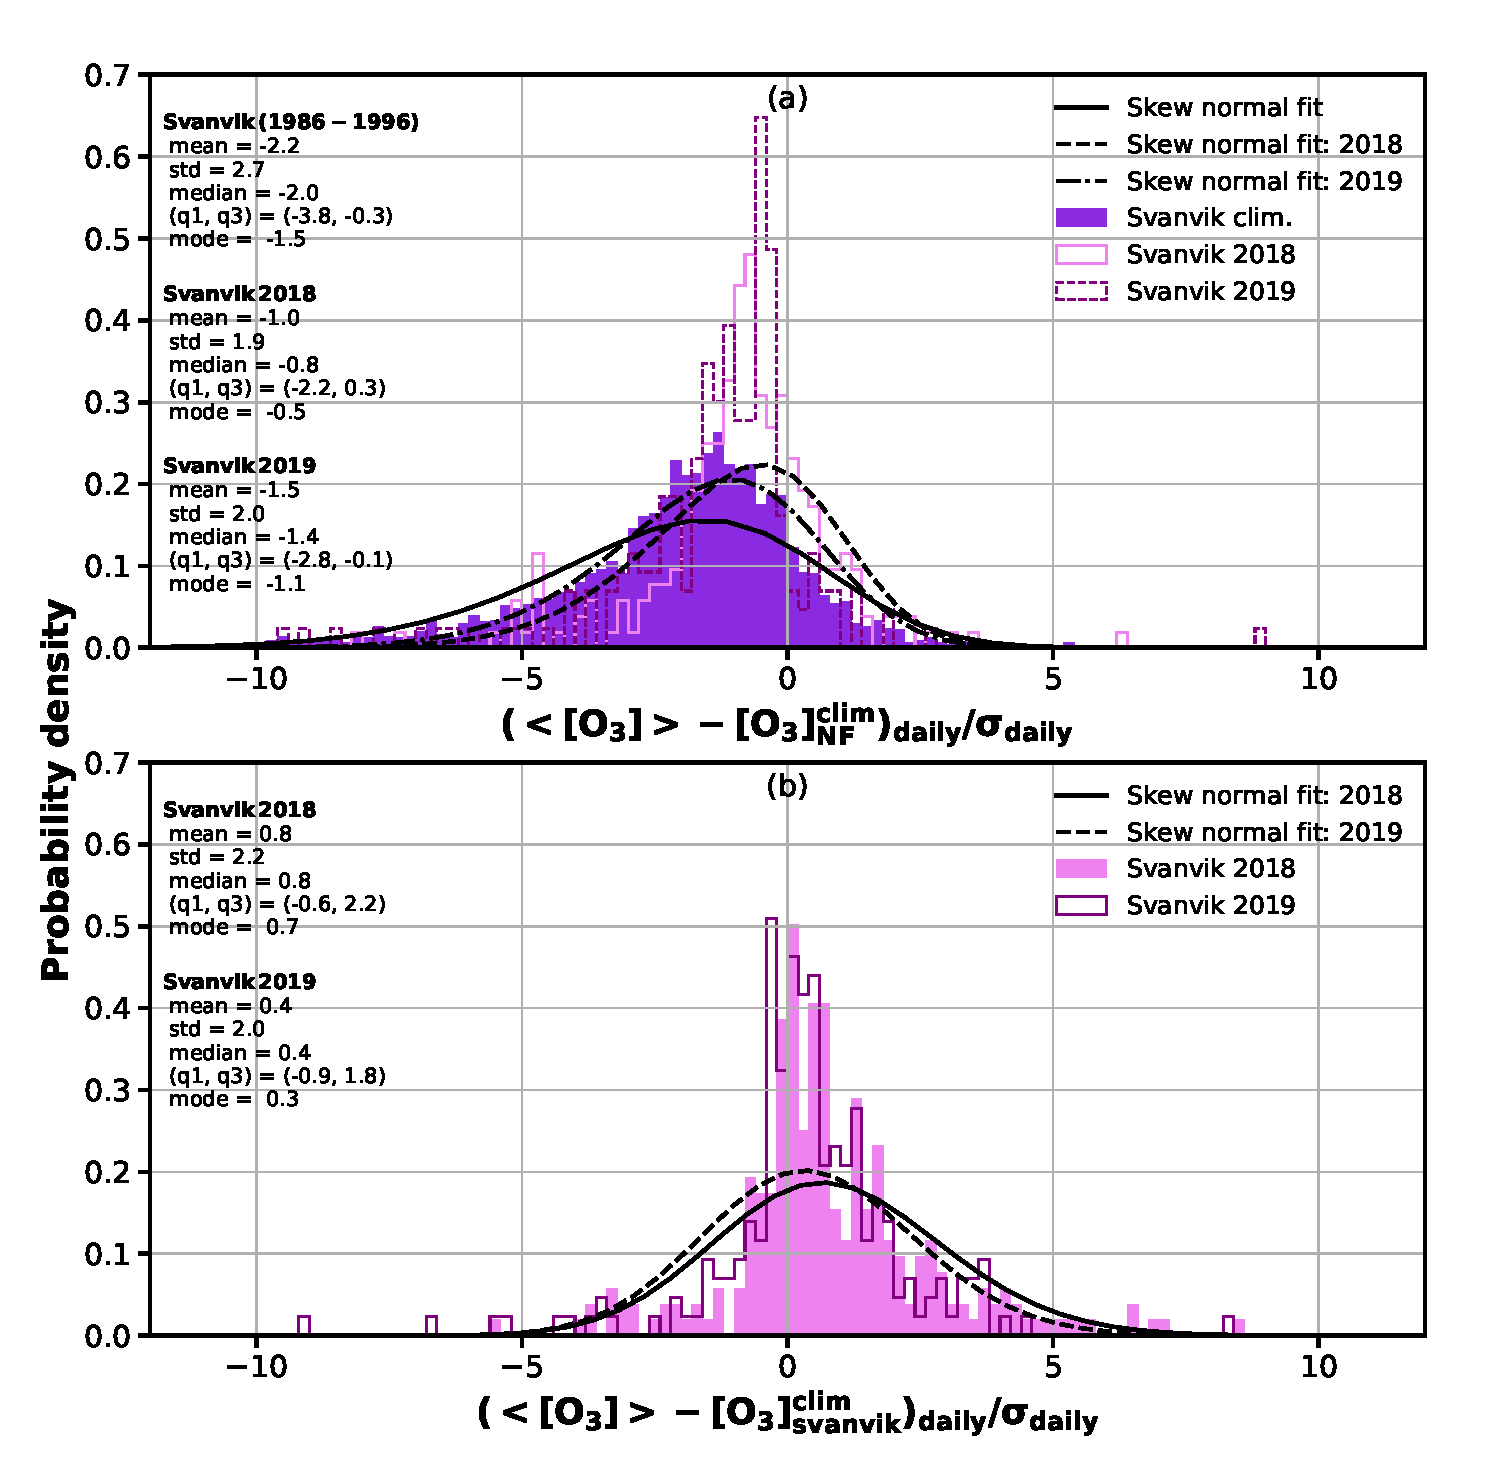
\includegraphics[width=12cm]{ozone_climatology_fenoscandic_obs_test-Svanvik}
  \caption{Student's t-test assuming same sample uncertainty in both, climatology and 2018/19 observations at Svanhovd with respect to derived climatologies for (a) Northern Fennoscandia; (b) Svanvik. \chem{\Delta[O_3]} in Fig.~\ref{fig:ozone_climatology_fenoscandic_obs_residuals}a) are significantly different from zero-hypothesis on the $2\,\sigma$,  $1\,\sigma$ level, respectively. \chem{\Delta[O_3]} in Fig.~\ref{fig:ozone_climatology_fenoscandic_obs_residuals}b) are not significantly different from zero-hypothesis.}
  \label{fig:ozone_climatology_fenoscandic_obs_test-Svanvik}
\end{figure*}

\begin{figure*}[t]
  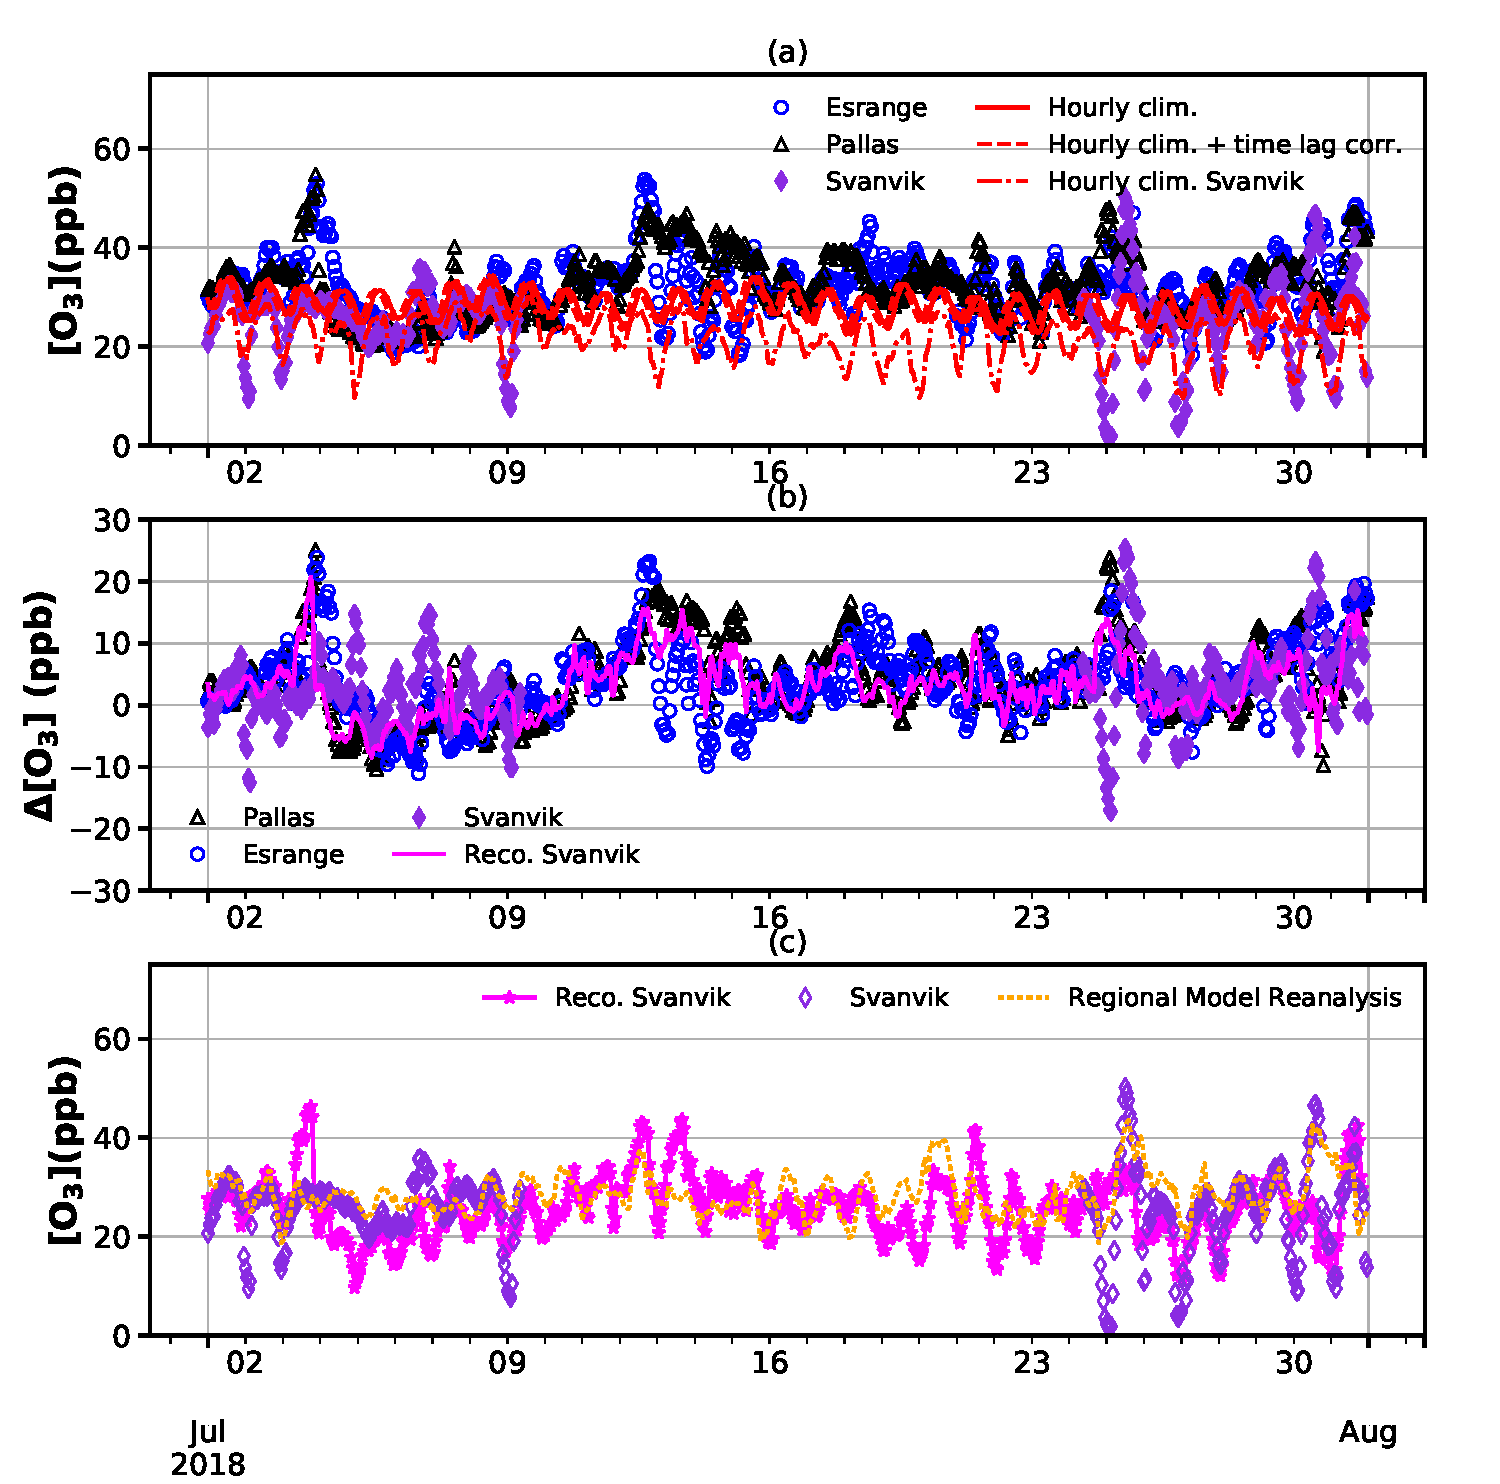
\includegraphics[width=12cm]{ozone_reconstruction_2018_07}
  \caption{Reconstruction of missing \chem{[O_3]} observation data at Svanvik in July 2018 based on derived hourly climatologies of northern Fennoscandia, Svanvik, and data Pallas. (a) Time series; (b) anomalies; (c) reconstruction.}
  \label{fig:ozone_reconstruction_2018_07}
\end{figure*}

\begin{figure*}[t]
  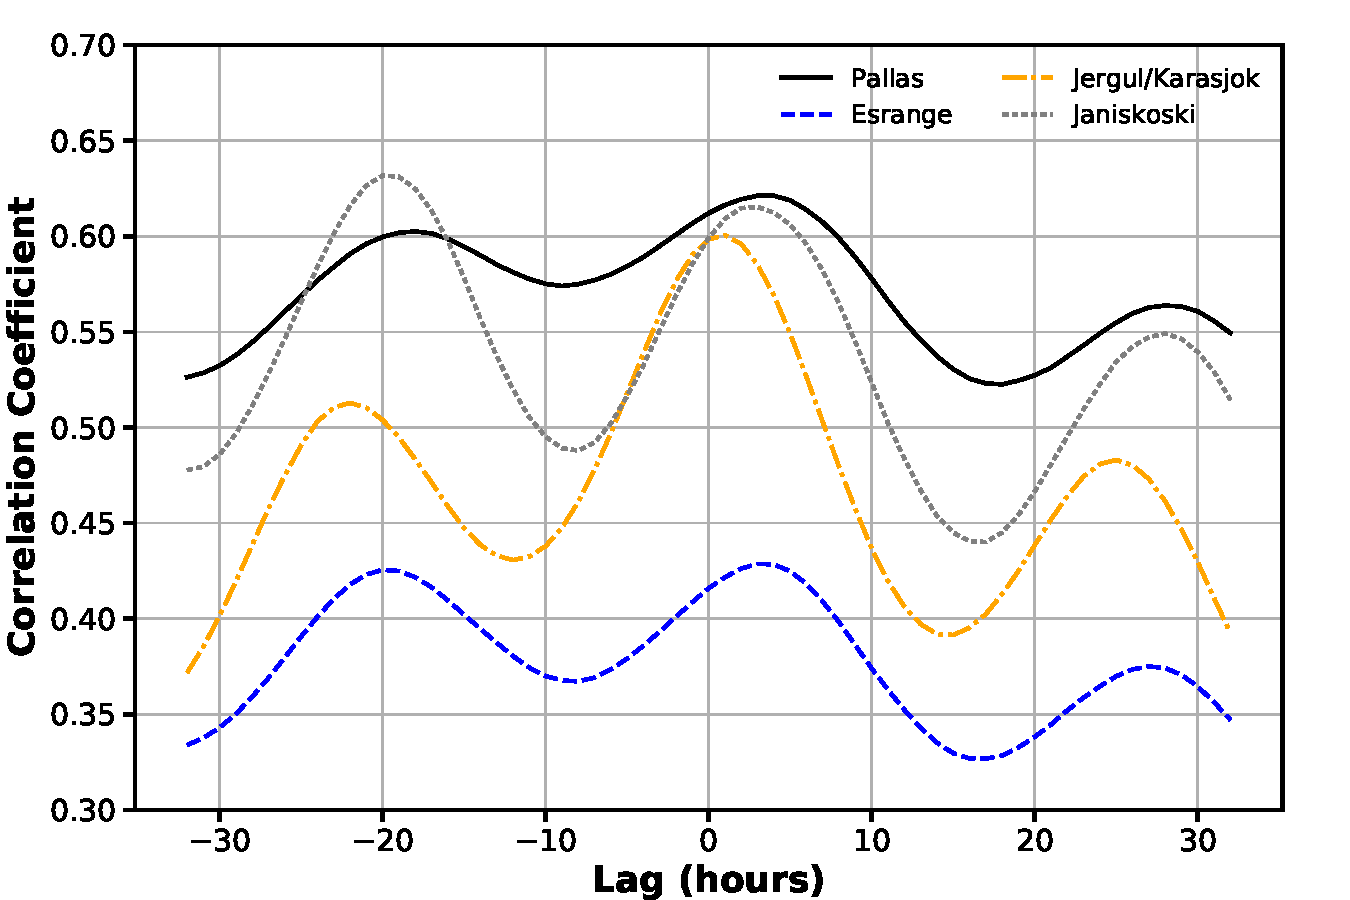
\includegraphics[width=12cm]{ozone_observation_timelag_svanvik}
  \caption{Temporal correlation of \chem{[O_3]} data at Svanvik with other ozone monitoring stations in northern Fennoscandia. A negative lag means that Svanvik lags behind, while a positive lag mean the other station lags behind. The highest correlation with Pallas/Esrange is found at a time lag of $3\,\unit{h}$, for Jergul/Karasjok at $1\,\unit{h}$, and for Janiskoski at $-20\,\unit{h}$.}
  \label{fig:time_lag_correlation}
\end{figure*}

% Shall go to supplement!
%\begin{figure*}[t]
%  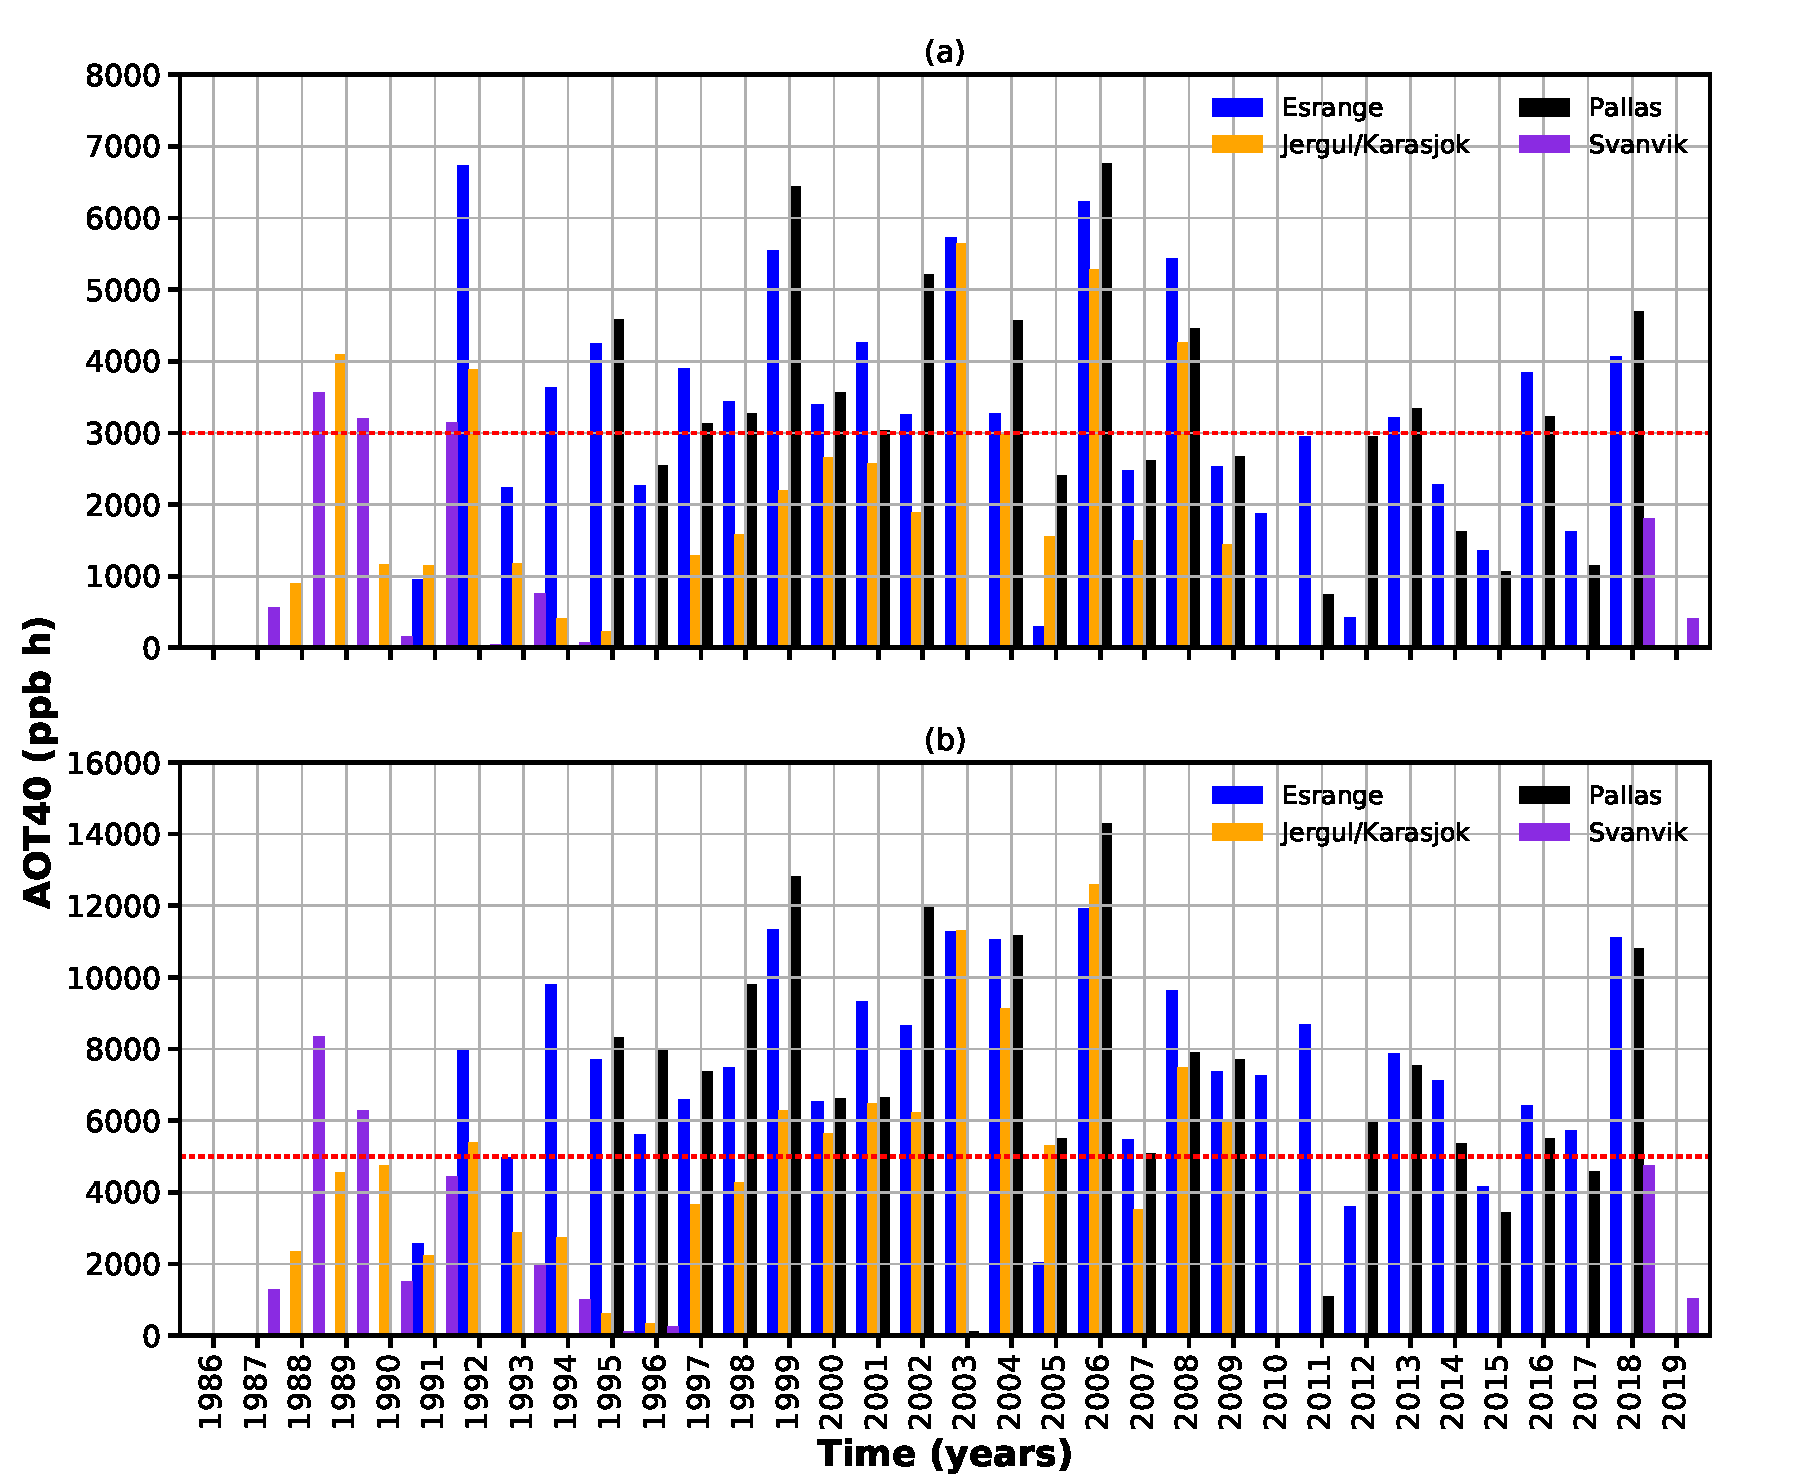
\includegraphics[width=12cm]{ozone_fennoscandic_obs_aot40}
%  \caption{Integrated AOT40 for various sites in northern Fennoscandia over the course of 33 years. For simplicity, we integrated hourly ozone between $1\,\unit{am}-11\,\unit{pm}$ in any case, although a night time light intensity $> 50\,\unit{W\,m^{-2}}$ is only measured during midnight sun conditions. Since night time \chem{[O_3]} is mostly below $40\,\unit{ppb}$, the such induced high bias in spring should be tolerable. The dashed red lines indicate the respective threshold given by the EU directive. (a) May 1 -- July 31 (b) April 1 -- September 30.}
%  \label{fig:fennoscandic_aot40}
%\end{figure*}

\begin{figure*}[t]
  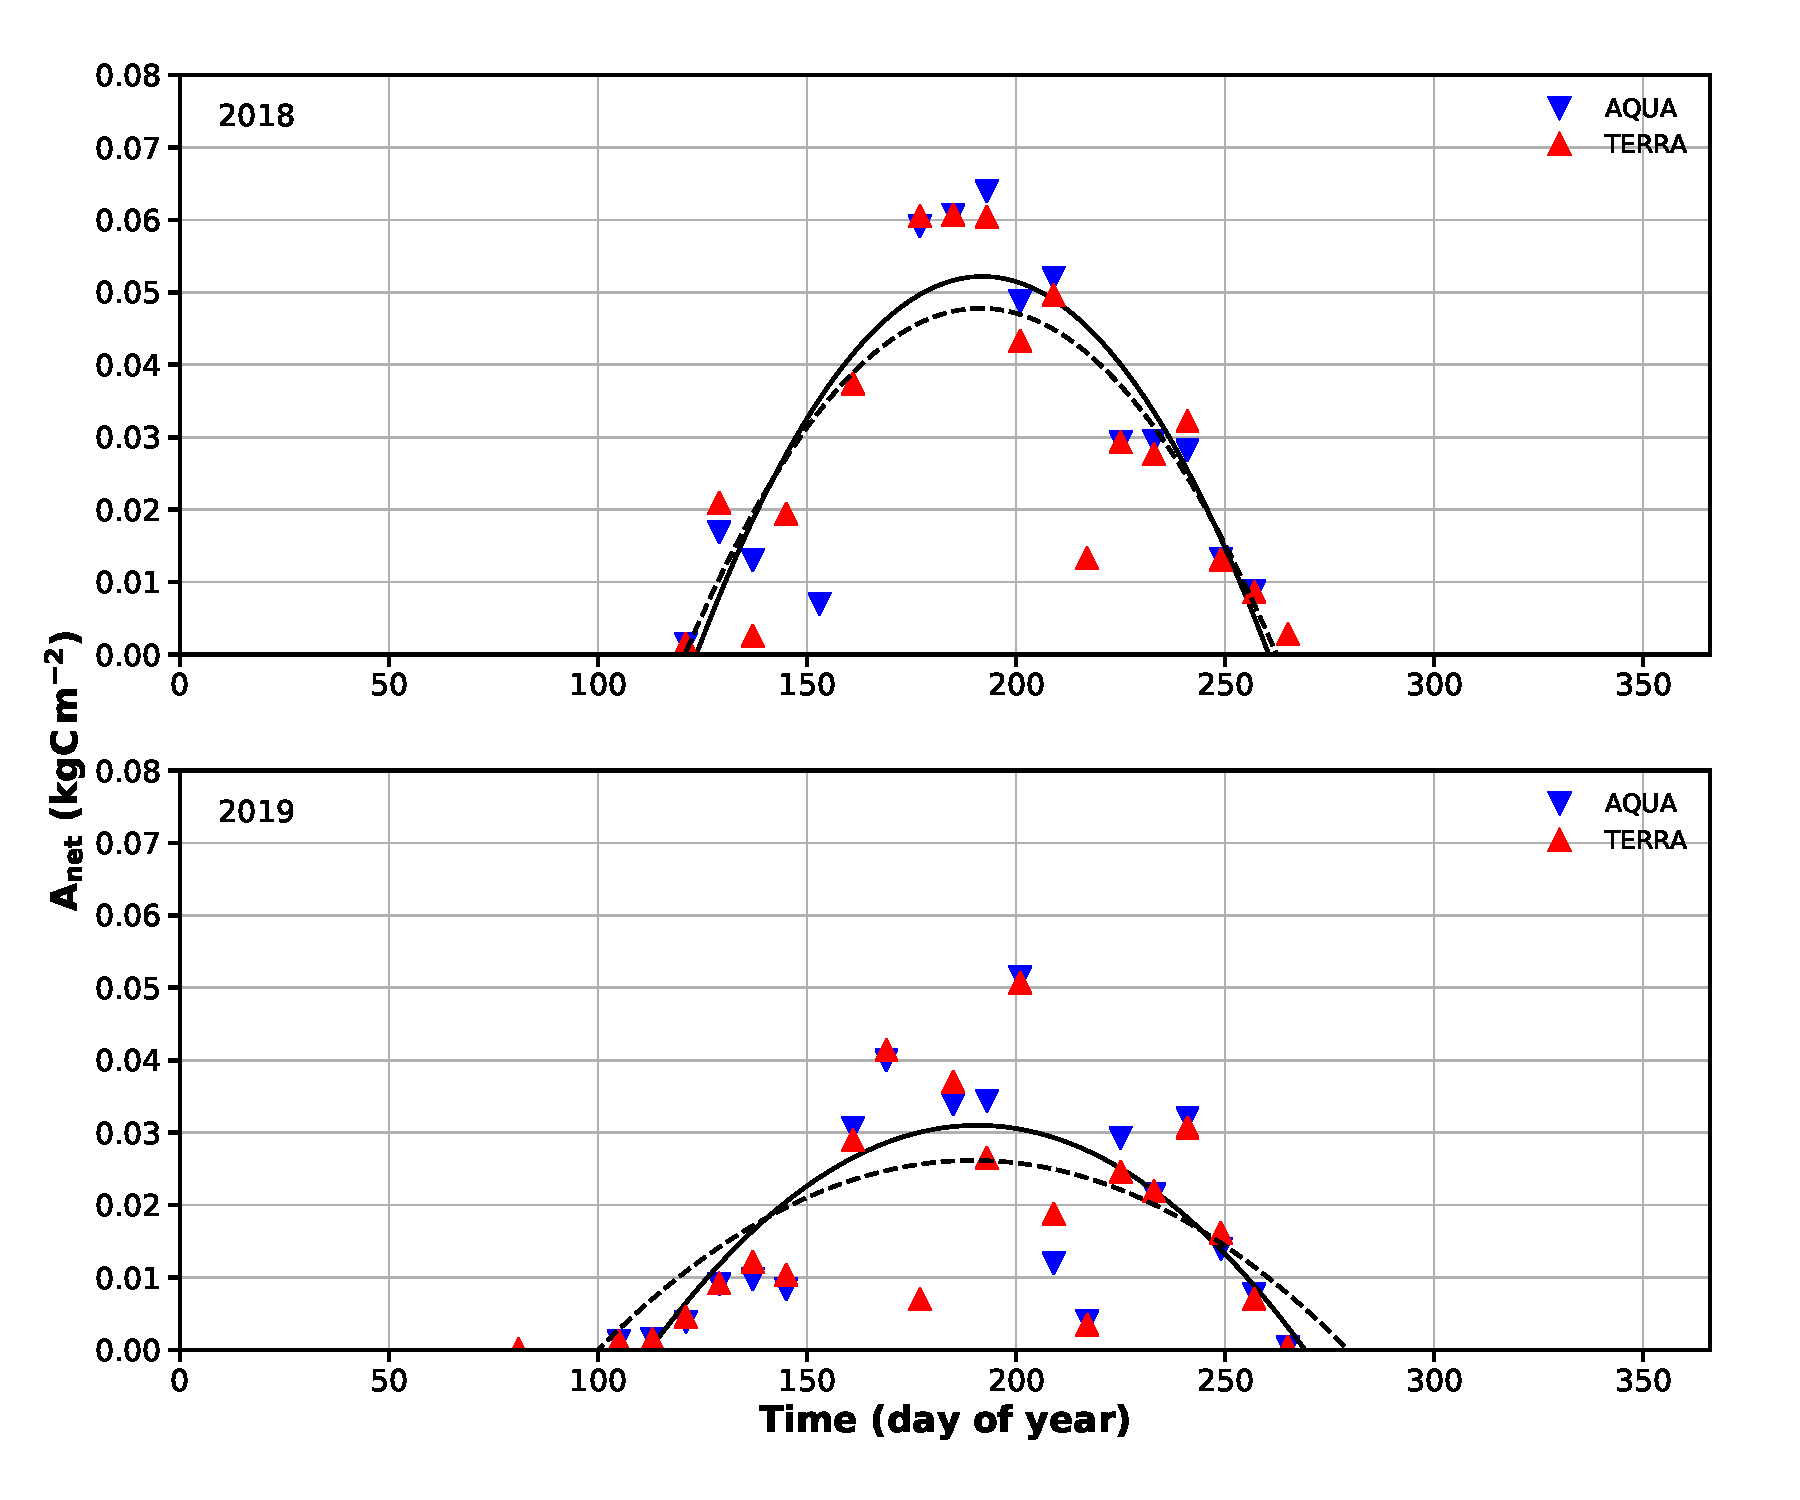
\includegraphics[width=12cm]{modis_Psn}
  \caption{Estimated begin (BGS) and end (EGS) of growing season for coniferous trees from MODIS Aqua/Terra net photosynthesis (PSN) product. A $1\times 1\,\unit{km}$ area around Svanhovd was selected. Daily averaged data for both 2018 and 2019 has been fitted with a quadratic polynomial function. The numerically computed root yields: BGS 122/106 day of year (doy) and EGS 261/274 day of year for 2018/2019, respectively.}
  \label{fig:modis_Psn}
\end{figure*}

\clearpage

\section{DO3SE parameterization}

\begin{figure}[t]
  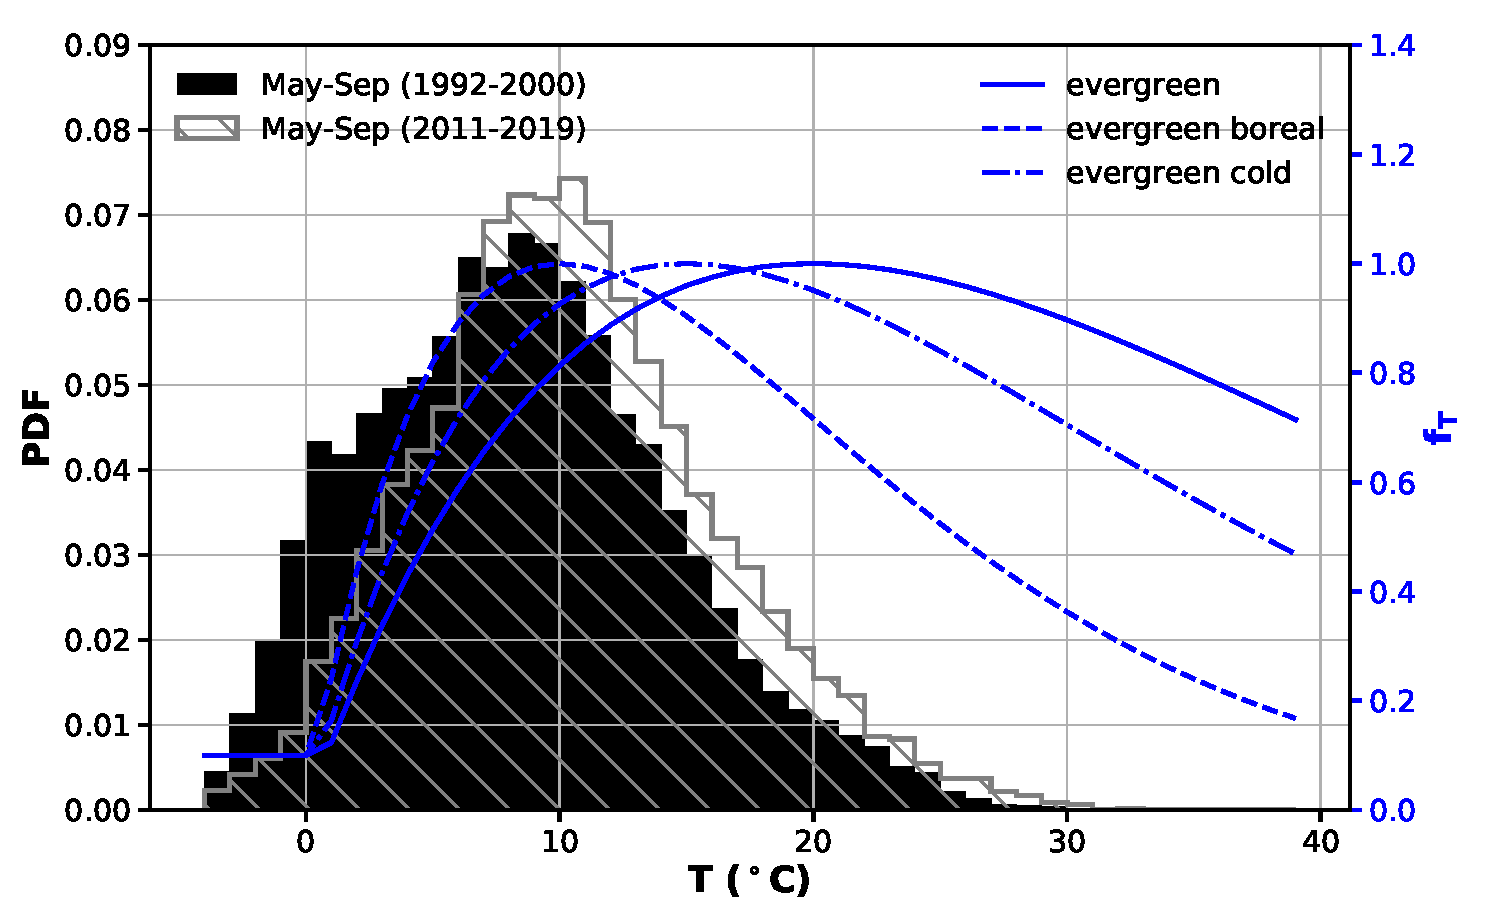
\includegraphics[width=8.3cm]{javis_funcs_temp_hist_evergreen}\\
  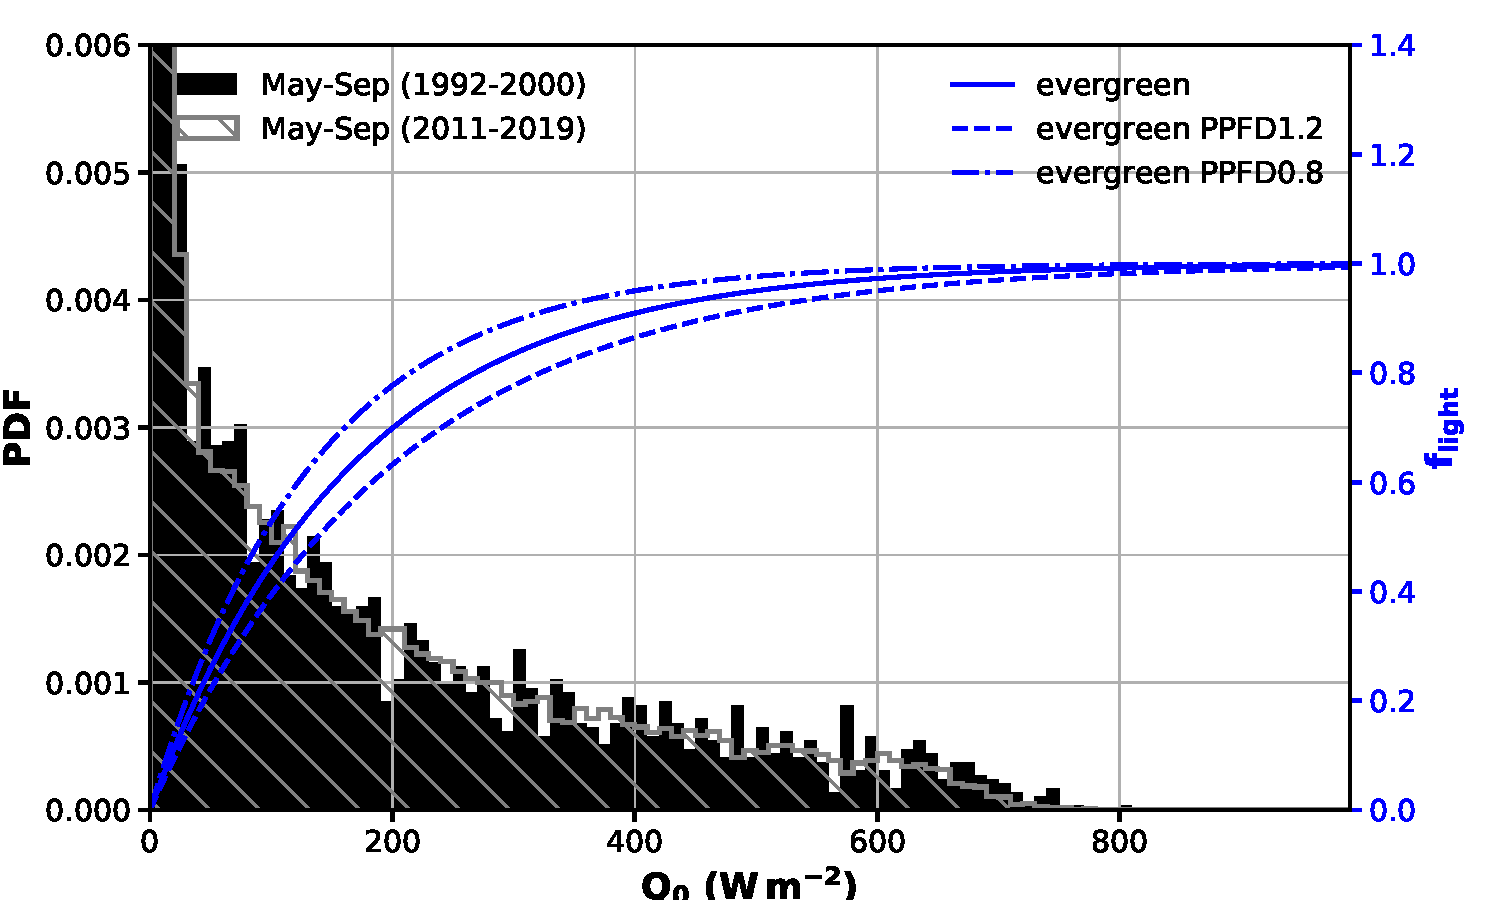
\includegraphics[width=8.3cm]{javis_funcs_rad_hist_evergreen}
\caption{Construction of bespoke response functions for Norway spruce. (a) $f_\mathrm{T}$ and (b) $f_\mathrm{flight}$ are shown toghether with underlying $T_\mathrm{air}$ and $Q_0$ climatologies (probability densitiy function - PDF), respectively. Original mapping manual parameterization is shown in comparison as solid line. Note that $Q_0$ has been truncated to $0.006$. PPFD0.8 and PPFD1.2 refer to $\alpha$ values increasing/decreasing PPFD at $f_\mathrm{light}=0.5$ by $\pm 20\,\%$, respectively.}
\label{fig:f_temp_spruce}
\end{figure}

\begin{figure}[t]
  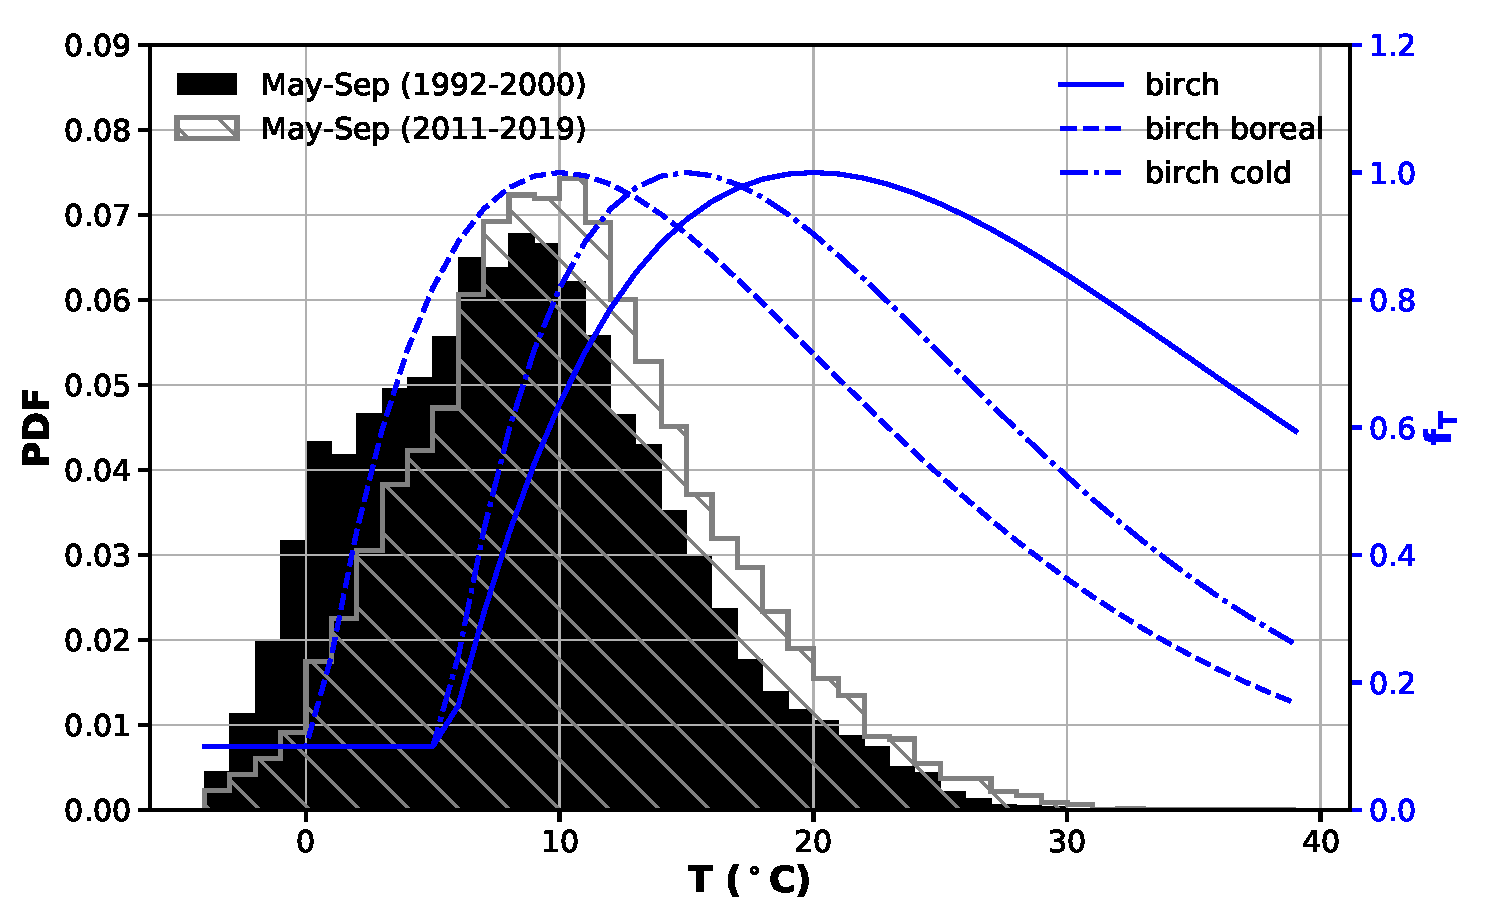
\includegraphics[width=8.3cm]{javis_funcs_temp_hist_birch}\\
  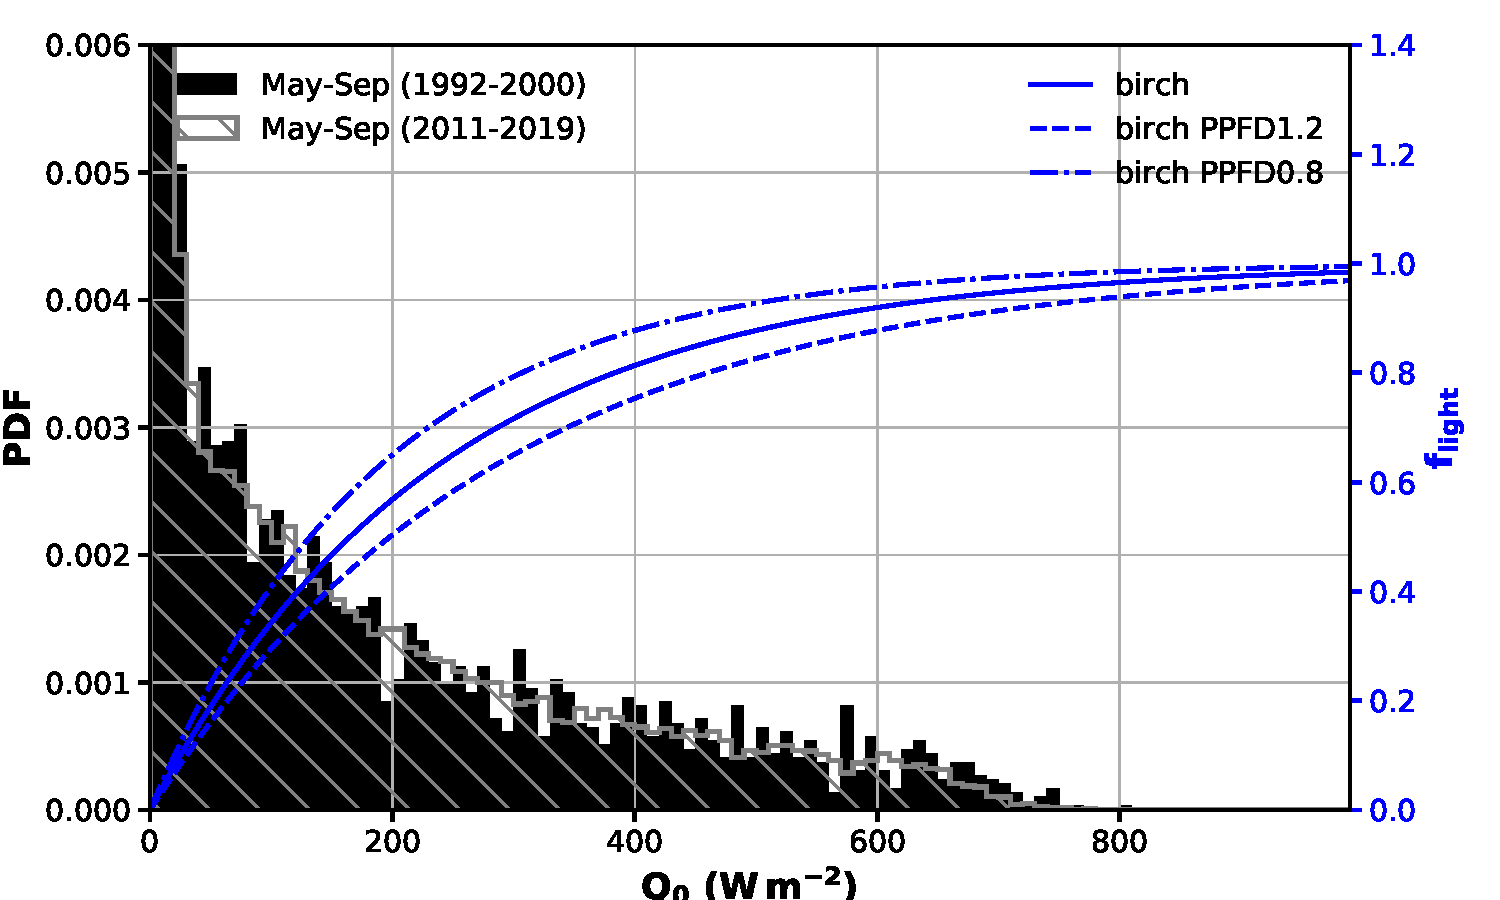
\includegraphics[width=8.3cm]{javis_funcs_rad_hist_birch}
\caption{Construction of bespoke response functions for Norway birch. (a) $f_\mathrm{T}$ and (b) $f_\mathrm{flight}$ are shown toghether with underlying $T_\mathrm{air}$ and $Q_0$ climatologies (probability densitiy function - PDF), respectively. Original mapping manual parameterization is shown in comparison as solid line. Note that $Q_0$ has been truncated to $0.006$. PPFD0.8 and PPFD1.2 refer to $\alpha$ values increasing/decreasing PPFD at $f_\mathrm{light}=0.5$ by $\pm 20\,\%$, respectively.}
\label{fig:f_temp_birch}
\end{figure}



\noappendix       %% use this to mark the end of the appendix section. Otherwise the figures might be numbered incorrectly (e.g. 10 instead of 1).

%% Regarding figures and tables in appendices, the following two options are possible depending on your general handling of figures and tables in the manuscript environment:

%% Option 1: If you sorted all figures and tables into the sections of the text, please also sort the appendix figures and appendix tables into the respective appendix sections.
%% They will be correctly named automatically.

%% Option 2: If you put all figures after the reference list, please insert appendix tables and figures after the normal tables and figures.
%% To rename them correctly to A1, A2, etc., please add the following commands in front of them:

%\appendixfigures  %% needs to be added in front of appendix figures


%\noappendix

%\appendixtables   %% needs to be added in front of appendix tables

%% Please add \clearpage between each table and/or figure. Further guidelines on figures and tables can be found below.



\authorcontribution{SF has written the manuscript, collected and processed ozone and environmental data, and performed all statistical analyses. AVV has performed on-site observation of vegetation damage induced by ozone and contributed to theory of ozone interaction with vegetation within the introduction. LE... CO... ALEB...  FS... TB... All authors contributed to discussion and conclusion of the results.} %% this section is mandatory

\competinginterests{The authors declare that they have no conflict of interest.} %% this section is mandatory even if you declare that no competing interests are present

%\disclaimer{TEXT} %% optional section

\begin{acknowledgements}
  Bj{\o}rg Rognerud for processing SeNorge.no data with respect for begin of growing season.
  Tore Flatlandsmo Berglen for hourly pressure data from Svanhovd.
\end{acknowledgements}




%% REFERENCES

%% The reference list is compiled as follows:

%\begin{thebibliography}{}

%\bibitem[AUTHOR(YEAR)]{LABEL1}
%REFERENCE 1

%\bibitem[AUTHOR(YEAR)]{LABEL2}
%REFERENCE 2

%\end{thebibliography}

%% Since the Copernicus LaTeX package includes the BibTeX style file copernicus.bst,
%% authors experienced with BibTeX only have to include the following two lines:
%%
\bibliographystyle{copernicus}
\bibliography{VegOzone.bib}
%%
%% URLs and DOIs can be entered in your BibTeX file as:
%%
%% URL = {http://www.xyz.org/~jones/idx_g.htm}
%% DOI = {10.5194/xyz}


%% LITERATURE CITATIONS
%%
%% command                        & example result
%% \citet{jones90}|               & Jones et al. (1990)
%% \citep{jones90}|               & (Jones et al., 1990)
%% \citep{jones90,jones93}|       & (Jones et al., 1990, 1993)
%% \citep[p.~32]{jones90}|        & (Jones et al., 1990, p.~32)
%% \citep[e.g.,][]{jones90}|      & (e.g., Jones et al., 1990)
%% \citep[e.g.,][p.~32]{jones90}| & (e.g., Jones et al., 1990, p.~32)
%% \citeauthor{jones90}|          & Jones et al.
%% \citeyear{jones90}|            & 1990



%% LITERATURE CITATIONS
%%
%% command                        & example result
%% \citet{jones90}|               & Jones et al. (1990)
%% \citep{jones90}|               & (Jones et al., 1990)
%% \citep{jones90,jones93}|       & (Jones et al., 1990, 1993)
%% \citep[p.~32]{jones90}|        & (Jones et al., 1990, p.~32)
%% \citep[e.g.,][]{jones90}|      & (e.g., Jones et al., 1990)
%% \citep[e.g.,][p.~32]{jones90}| & (e.g., Jones et al., 1990, p.~32)
%% \citeauthor{jones90}|          & Jones et al.
%% \citeyear{jones90}|            & 1990



%% FIGURES

%% When figures and tables are placed at the end of the MS (article in one-column style), please add \clearpage
%% between bibliography and first table and/or figure as well as between each table and/or figure.

% The figure files should be labelled correctly with Arabic numerals (e.g. fig01.jpg, fig02.png).


%% ONE-COLUMN FIGURES

%%f
%\begin{figure}[t]
%\includegraphics[width=8.3cm]{FILE NAME}
%\caption{TEXT}
%\end{figure}
%
%%% TWO-COLUMN FIGURES
%
%%f
%\begin{figure*}[t]
%\includegraphics[width=12cm]{FILE NAME}
%\caption{TEXT}
%\end{figure*}
%
%
%%% TABLES
%%%
%%% The different columns must be seperated with a & command and should
%%% end with \\ to identify the column brake.
%
%%% ONE-COLUMN TABLE
%
%%t
%\begin{table}[t]
%\caption{TEXT}
%\begin{tabular}{column = lcr}
%\tophline
%
%\middlehline
%
%\bottomhline
%\end{tabular}
%\belowtable{} % Table Footnotes
%\end{table}
%
%%% TWO-COLUMN TABLE
%
%%t
%\begin{table*}[t]
%\caption{TEXT}
%\begin{tabular}{column = lcr}
%\tophline
%
%\middlehline
%
%\bottomhline
%\end{tabular}
%\belowtable{} % Table Footnotes
%\end{table*}
%
%%% LANDSCAPE TABLE
%
%%t
%\begin{sidewaystable*}[t]
%\caption{TEXT}
%\begin{tabular}{column = lcr}
%\tophline
%
%\middlehline
%
%\bottomhline
%\end{tabular}
%\belowtable{} % Table Footnotes
%\end{sidewaystable*}
%
%
%%% MATHEMATICAL EXPRESSIONS
%
%%% All papers typeset by Copernicus Publications follow the math typesetting regulations
%%% given by the IUPAC Green Book (IUPAC: Quantities, Units and Symbols in Physical Chemistry,
%%% 2nd Edn., Blackwell Science, available at: http://old.iupac.org/publications/books/gbook/green_book_2ed.pdf, 1993).
%%%
%%% Physical quantities/variables are typeset in italic font (t for time, T for Temperature)
%%% Indices which are not defined are typeset in italic font (x, y, z, a, b, c)
%%% Items/objects which are defined are typeset in roman font (Car A, Car B)
%%% Descriptions/specifications which are defined by itself are typeset in roman font (abs, rel, ref, tot, net, ice)
%%% Abbreviations from 2 letters are typeset in roman font (RH, LAI)
%%% Vectors are identified in bold italic font using \vec{x}
%%% Matrices are identified in bold roman font
%%% Multiplication signs are typeset using the LaTeX commands \times (for vector products, grids, and exponential notations) or \cdot
%%% The character * should not be applied as mutliplication sign
%
%
%%% EQUATIONS
%
%%% Single-row equation
%
%\begin{equation}
%
%\end{equation}
%
%%% Multiline equation
%
%\begin{align}
%& 3 + 5 = 8\\
%& 3 + 5 = 8\\
%& 3 + 5 = 8
%\end{align}
%
%
%%% MATRICES
%
%\begin{matrix}
%x & y & z\\
%x & y & z\\
%x & y & z\\
%\end{matrix}
%
%
%%% ALGORITHM
%
%\begin{algorithm}
%\caption{...}
%\label{a1}
%\begin{algorithmic}
%...
%\end{algorithmic}
%\end{algorithm}
%
%
%%% CHEMICAL FORMULAS AND REACTIONS
%
%%% For formulas embedded in the text, please use \chem{}
%
%%% The reaction environment creates labels including the letter R, i.e. (R1), (R2), etc.
%
%\begin{reaction}
%%% \rightarrow should be used for normal (one-way) chemical reactions
%%% \rightleftharpoons should be used for equilibria
%%% \leftrightarrow should be used for resonance structures
%\end{reaction}
%
%
%%% PHYSICAL UNITS
%%%
%%% Please use \unit{} and apply the exponential notation


\end{document}
